\documentclass[lang=cn,a4paper,11pt,openany,twoside]{elegantbook}

\let\arrowvert\relax
%\usepackage{unicode-math}

\let\arrowvert\relax

\usepackage{ctex}
\usepackage{xeCJK}

\let\fangsong\relax
\newCJKfontfamily\fangsong{FangSong}[AutoFakeBold=2]

\let\kaishu\relax
\newCJKfontfamily\kaishu{KaiTi}[AutoFakeBold=2]


\usepackage{amsmath} % 建议
\usepackage{amssymb} % 可选，提供更多符号

\usepackage{ctex}
\let\openbox\relax

\usepackage{tikz}
\usetikzlibrary{decorations.pathreplacing,arrows.meta}

%调整页边距
\usepackage{geometry}
\geometry{top=2cm, bottom=2.25cm, outer=2cm, inner=2.5cm}


\usepackage{setspace}
\setstretch{1.3}

%设定行间距
\usepackage{calc}
\setlength{\lineskip}{\baselineskip-\ccwd}
\setlength{\lineskiplimit}{2.5pt}

\usepackage{fontspec}

\usepackage{paratype}


\usepackage{amsfonts}
\usepackage{amssymb}
\usepackage{esint}

\usepackage{graphicx}
\usepackage[export]{adjustbox}
\usepackage{mdframed}
\usepackage{booktabs,array,multirow}
\usepackage{adjustbox}
\usepackage{tabularx}
\usepackage{hyperref}
\hypersetup{colorlinks=true, linkcolor=blue, filecolor=magenta, urlcolor=cyan,}
\urlstyle{same}
\usepackage{tcolorbox}
\graphicspath{ {./images/} }
\newcommand{\HRule}{\begin{center}\rule{0.9\linewidth}{0.2mm}\end{center}}
\newcommand{\customfootnote}[1]{
  \let\thefootnote\relax\footnotetext{#1}
}

%分式使用行间版
\everymath{\displaystyle}


\usepackage{myenvironment}


%elegantbook部分修改
\usepackage{elegantfix}

\newcommand\setboxcounter[2]{\setcounter{tcb@cnt@#1}{#2}}


%强制右页开始
\makeatletter
\newcommand{\ForceRightPage}{%
  \clearpage
  \ifodd\value{page}\relax
    % 已经是奇数页，什么也不做
  \else
    \hbox{}\thispagestyle{empty}\newpage
  \fi
}
\makeatother

\raggedbottom

\begin{document}

\title{本科代数几何}
\maketitle

\chapter*{前言}
\markboth{Introduction}{前言}

目前有几本优秀的研究生代数几何教材，但据我所知，没有专为本科课程设计的教材.这些简陋的讲义来自华威大学本科数学三年级连续两年开设的课程，旨在作为一本自成体系的入门教材.

\frontmatter
\pagenumbering{roman}     % 目录等用罗马数字
\clearpage
\tableofcontents
\clearpage

\ForceRightPage
\mainmatter

\chapter*{旧目录}

\section*{第零部分\quad 绪论} 研究代数几何的理由，“子集”问题；几何的不同范畴，交换代数的必要性，部分定义函数；作者特点.先修知识，与其他课程的关系，书目列表.

\section*{第一部分\quad 平面曲线的游戏}

\noindent
\textbf{1. 平面二次曲线}\;  对 \({\mathbb{P}}^{2}\) 和齐次坐标的基本熟悉， \({\mathbb{A}}^{2}\) 与 \({\mathbb{P}}^{2}\) 的关系；参数化，每个光滑二次曲线 \(C \subset  {\mathbb{P}}^{2}\) 都是 \(\cong  {\mathbb{P}}^{1}\) .贝祖定理的简单情况:直线 \(\cap\) 与 \(d = d\) 次曲线的交点，二次曲线 \(\cap\) 与 \(d = {2d}\) 次曲线的交点；通过 \({P}_{1},\ldots ,{P}_{n}\) 的二次曲线线性系统.

\noindent
\textbf{2. 三次曲线与群运算律}\; 曲线 \(\left( {{y}^{2} = x\left( {x - 1}\right) \left( {x - \lambda }\right) }\right)\) 无有理参数化.线性系统 \({S}_{d}\left( {{P}_{1},\ldots ,{P}_{n}}\right)\) ；通过8个“一般位置”点的三次曲线铅笔；三次曲线上的群律；帕斯卡神秘六边形.第一部分附录.曲线及其亏格(genus)

非奇异平面三次曲线在 \(\mathbb{C}\) 上的拓扑；曲线亏格的非正式讨论；拓扑、微分几何、模空间、数论、莫德尔-韦尔-法尔廷斯定理.

\section*{第二部分\quad 仿射簇的范畴}
\noindent
\textbf{3. 仿射簇与零点定理(Nullstellensatz)}\; 诺特环，希尔伯特基定理； \(V\) 与 \(I\) 的对应关系，不可约代数集，Zariski拓扑，零点定理陈述；不可约超曲面.诺特正规化及零点定理证明；归约到超曲面.

\noindent
\textbf{4. 簇上的函数}\; 坐标环与多项式映射；态射与同构；仿射簇.有理函数域与有理映射；占优有理映射及有理映射的复合；标准开集；椭圆曲线上的加法律是态射.

\section*{第三部分\quad 应用}
\noindent
\textbf{5. 射影簇与双有理等价}\; 动机:存在严格大于任何仿射簇的簇；齐次 \(V - I\) 对应；射影与仿射的对比.例子:二次曲面；Veronese曲面.双有理等价，有理簇；每个簇双有理等价于超曲面；积簇.

\noindent
\textbf{6. 切空间与非奇异性，维数}\; 动机:隐函数定理，簇与流形.仿射切空间的定义；非奇异点稠密.切空间与 \(m/{m}^{2}\) ，切空间是内在的； \(X = \operatorname{tr}{\deg }_{k}k\left( X\right)\) 的维数.通过爆破消除奇异点.

\noindent
\textbf{7. 三次曲面上的27条直线}\; 非奇异三次曲面上的直线 \(S\) .通过消元法证明直线的存在；极形式.与给定直线相交的5对直线. \(S\) 是有理的.27条直线的经典构型.黑塞矩阵.所有直线均为有理直线的情况.

\noindent
\textbf{8. 结语}\; 历史与社会学.选题，深奥评论与技术注释.代替前言；致谢与点名.

\setcounter{chapter}{-1}
\chapter{绪论}

本节旨在作为文化导入，逻辑上不属于课程内容，可略读.

\section{内容简介}

代数簇(variety)大致可以定义为由多项式方程族定义的轨迹:

\[
V = \left\{  {P \in  {k}^{n} \mid  {f}_{i}\left( P\right)  = 0}\right\}   \subset  {k}^{n},
\]

其中 \(k\) 是一个域， \({f}_{i} \in  k\left\lbrack  {{X}_{1},\ldots ,{X}_{n}}\right\rbrack\) 是多项式；例如，平面曲线 \(C\) : \(\left( {f\left( {x,y}\right)  = 0}\right)  \subset  {\mathbb{R}}^{2}\) 或 \({\mathbb{C}}^{2}\) .

\begin{center}
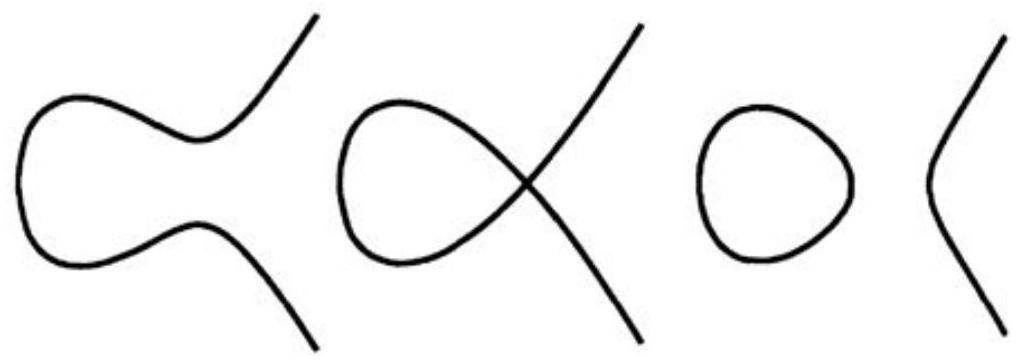
\includegraphics[max width=0.8\textwidth]{images/bo_d3lj80c601uc738kffi0_8_333_1201_1024_361_0.jpg}
\captionof{figure}{三次曲线 (a) \({y}^{2} = \left( {x + 1}\right) \left( {{x}^{2} + \varepsilon }\right) ,\;\) (b) \({y}^{2} = \left( {x + 1}\right) {x}^{2}\)，(c) \({y}^{2} = \left( {x + 1}\right) \left( {{x}^{2} - \varepsilon }\right)\)}.
\end{center}


如果我想研究 \(V\)，自然会产生以下几个问题:

\textbf{数论问题}\quad 例如，如果 \(k = \mathbb{Q}\) 和 \(V \subset  {\mathbb{Q}}^{n}\) ，如何判断 \(V\) 是否非空，若非空如何找到所有点？一个具体案例在历史上颇具意义：下列方程解的个数问题
\[
{x}^{n} + {y}^{n} = 1\text{ ,其中}x,y \in  \mathbb{Q}\text{且}n \geq  3\text{ ? }
\]

此类问题通常称为丢番图问题(Diophantine problems).

\textbf{拓扑问题}\quad 如果 \(k\) 是 \(\mathbb{R}\) 或 \(\mathbb{C}\) (常见情形)，那么 \(V\) 是什么样的拓扑空间？例如，上述三次曲线的连通分支就是明显的拓扑不变量.

\textbf{奇异性问题}\quad \(V\) 在 \(P \in  V\) 附近是什么样的拓扑空间；如果 \(f : {V}_{1} \rightarrow  {V}_{2}\) 是两个簇之间的正则映射(例如，多项式映射 \({\mathbb{R}}^{2} \rightarrow  \mathbb{R}\) )，那么 \(f\) 在 \(P \in  {V}_{1}\) 附近具有怎样的拓扑和几何结构？

\section{具体计算与一般理论}

研究簇有两种可能的方法:

具体的 给定特定的多项式 \({f}_{i}\) ，我们常常可以通过对 \({f}_{i}\) 的显式技巧来理解簇 \(V\) ；当维数 \(n\) 和 \({f}_{i}\) 的次数较小时，或者 \({f}_{i}\) 特别简单时，这很有趣，但情况会逐渐复杂，很快就会出现仅凭计算的巧思无法揭示问题本质的时刻.

一般的 对 \(V\) 性质的研究立即引出基本概念，如 \(V\) 上的正则函数(regular functions)、非奇异性(nonsingularity)和切平面、簇的维数:曲线如上述三次曲线是一维的这一观念在初等笛卡尔几何中很熟悉，图像也立即暗示了奇异点的含义.

现在，开设本科代数几何课程的一个基本问题是，对“通用”方法的充分讲解涉及大量定义，这些定义占满整个课程，挤压了实质内容.因此必须妥协，我的解决方案是覆盖一般理论的一小部分，并不断参照具体例子.因此这些讲义仅包含构成三年本科数学课程中专门代数几何必修核心的“标准教材”内容的一小部分.另一方面，我希望每节都包含一些有实质内容的习题和例题.

\section{函数环与几何范畴}

代数几何的特殊风格源于仅使用多项式函数(以及有理函数)；为说明这一点，若 \(U \subset  {\mathbb{R}}^{2}\) 是一个开区间，则可以合理地考虑以下定义在 \(U\) 上的函数环:

\begin{itemize}
\item \({C}^{0}\left( U\right)  =\) 所有连续函数 \(f : U \rightarrow  \mathbb{R}\) ；
\end{itemize}

\begin{itemize}
\item \({C}^{\infty }\left( U\right)  =\) 所有光滑函数(即任意阶可微)；
\end{itemize}

\begin{itemize}
\item \({C}^{\omega }\left( U\right)  =\) 所有解析函数(即收敛幂级数)；
\end{itemize}

\begin{itemize}
\item \(\mathbb{R}\left\lbrack  X\right\rbrack   =\) 多项式环，视为定义在 \(U\) 上的多项式函数.
\end{itemize}

当然存在包含关系 \(\mathbb{R}\left\lbrack  X\right\rbrack   \subset  {C}^{\omega }\left( U\right)  \subset  {C}^{\infty }\left( U\right)  \subset  {C}^{0}\left( U\right)\) .

这些函数环对应于几何学中的一些重要范畴: \({C}^{0}\left( U\right)\) 对应拓扑范畴， \({C}^{\infty }\left( U\right)\) 对应可微范畴(可微流形)， \({C}^{\omega }\) 对应实解析几何， \(\mathbb{R}\left\lbrack  X\right\rbrack\) 对应代数几何.我想强调的是，每一个包含符号都代表着一个极其巨大的鸿沟，这导致了不同范畴中几何的主要特征.虽然在学校和大学一年级的微积分中并未强调，但任何合理的测度方式 \({C}^{0}\left( U\right)\) 都会显示可微函数在连续函数中测度为零(因此如果随机选取一个连续函数，几乎必然处处不可微，如布朗运动). \({C}^{\omega }\left( U\right)\) 与 \({C}^{\infty }\left( U\right)\) 之间的差距通过标准函数 \(\exp \left( {-1/{x}^{2}}\right)\) 的行为得以体现，该函数可微无数次，但其在0点的泰勒级数不收敛于 \(f\) ；利用此函数，可以轻松构造一个 \({C}^{\infty }\) “凸起函数” \(f : \mathbb{R} \rightarrow  \mathbb{R}\) ，使得当 \(\left| x\right|  \leq  {0.9}\) 时 \(f\left( x\right)  = 1\) ，当 \(\left| x\right|  \geq  1\) 时 \(f\left( x\right)  = 0\) .相比之下，定义在 \(U\) 上的解析函数可作为复变量的解析函数(幂级数收敛)延拓到 \({C}^{0}\left( U\right)\) 中合适的区域，因此(利用复分析的结果)，如果 \({C}^{\infty }\left( U\right)\) 在实区间上恒为零，则必在整体上恒为零.这是一种“刚性”性质，区别了解析几何与微分拓扑.

\begin{center}
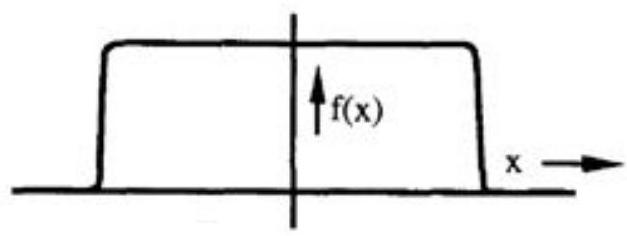
\includegraphics[max width=0.4\textwidth]{images/bo_d3lj80c601uc738kffi0_10_531_651_627_236_0.jpg}
\end{center}
\hspace*{3em} 

图2:一个 \({C}^{\infty }\) 凸起函数.

幂级数)延拓为复变量的解析函数，定义在 \(\mathbb{C}\) 中合适的区域，因此(利用复分析的结果)，如果 \(f \in  {C}^{\omega }\left( U\right)\) 在实区间上恒为零，则必在整体上恒为零.这是一种“刚性”性质，区别了解析几何与微分拓扑.

\section{多项式几何}

多项式函数非常稀少:多项式环 \(\mathbb{R}\left\lbrack  X\right\rbrack\) 只是一个可数维的 \(\mathbb{R}\) -向量空间，而 \({C}^{\omega }\left( U\right)\) 已经是不可数的.即使允许有理函数——即将 \(\mathbb{R}\left\lbrack  X\right\rbrack\) 扩展到其分式域 \(\mathbb{R}\left( X\right)\) ——也帮助不大.(2.2)将提供代数范畴特有刚性的一个例子.仅用这组函数构建几何本身就相当了不起.不出所料，建立这一理论存在诸多困难:

通过交换代数的基础 拓扑学和微分拓扑学可以依赖于一系列 \(\varepsilon  - \delta\) 分析课程中教授的全部内容，这些课程通常为 \(1\mathrm{{st}}\) 和 \(2\mathrm{{nd}}\) 年制的本科课程；而要仅用多项式环来进行代数几何研究，我们则需要研究诸如多项式环 \(k\left\lbrack  {{X}_{1},\ldots ,{X}_{n}}\right\rbrack\) 及其理想等环.换句话说，我们必须发展交换代数以替代微积分.Nullstellensatz(下文的 \(§3\) )是一个典型例子，它是一个具有直接直观几何内容的命题(本质上是“多项式环 \(k\left\lbrack  {{X}_{1},\ldots ,{X}_{n}}\right\rbrack\) 中不同的函数理想定义不同的簇(varieties) \(V \subset  {k}^{n}\) ”)，其证明涉及交换代数中有限性条件的较长论述.

有理映射和函数 由于选择仅用多项式进行研究，另一个难点是必须引入“部分定义的函数”；正如上文所暗示的“刚性”，我们将看到对于某些簇(实际上是所有射影簇)，不存在任何非恒定的正则函数(参见例5.1、例5.12及(8.10)中的讨论).有理函数(即形如 \(f = g/h\) 的“函数”，其中 \(g,h\) 是多项式函数)在分母为零的点处未定义.尽管令人诟病，但代数几何学家中有一种根深蒂固的传统，将“有理函数”和“有理映射”理解为“仅部分定义的函数(或映射)”.因此，有理映射 \(f : {V}_{1} \rightarrow  {V}_{2}\) 实际上根本不是映射；这里的断箭头也逐渐成为惯例.不赞同者建议立即放弃，转而选修范畴论的阅读课程.

这绝非轻率的问题.即使是正则映射(即态射，是真正的映射)也必须定义为在所有点 \(P \in  V\) 处正则的有理映射(即定义良好，分母可选取为在 \(P\) 处不为零).与此密切相关的是给出簇的恰当内在定义的难题:在本课程(以及我所知的类似课程)中，将定义仿射簇 \(V \subset  {\mathbb{A}}^{n}\) 和拟射影簇 \(V \subset  {\mathbb{P}}^{n}\) ，但不会给出不依赖于环境空间的“簇”的恰当定义.粗略地说，簇应当是将若干仿射簇沿同构的开子集粘合而成的对象.但我们目前的语言中，同构本身多半是通过有理函数明确定义的，过于繁琐；而这种粘合的恰当语言是层(sheaves)，这在研究生教材中有较好论述.

\section{“纯代数定义”}

以上即代数几何方法的缺点.话虽如此，现今世界上几乎所有重要的代数簇都是拟射影簇，我们可以在不太纠结定义细节的情况下，尽情享受簇的乐趣.

代数几何的主要优势在于它是纯代数定义的，且适用于任意域，而不仅仅是 \(\mathbb{R}\) 或 \(\mathbb{C}\) ；我们可以在特征为 \(p\) 的域上做几何.不要说“特征为 \(p\) ——没什么大不了的，那只是有限域”；首先，群论中相当重要的部分基于有限域上的几何，计算机科学中使用的组合学的很大一部分也是如此.其次，存在许多有趣的非有限的特征为 \(p\) 的域.此外，在深层次上，有限域存在并作用于 \(\mathbb{Q}\) 和 \(\mathbb{C}\) 中.关于在 \(\mathbb{Q}\) 上的簇的算术的许多深刻结果，都大量使用了在 \(\mathbb{C}\) 或有限域及其代数闭包上的几何.

介绍到此结束；更多通识内容请参见(2.15)中的非正式讨论及最后的 \(§8\) .

\section{本书计划}

关于本书的结构，第一部分和第三部分旨在指出一些可以通过代数几何方法研究的有价值的问题.第二部分是对(0.4)中提到的交换代数及代数几何的范畴框架的介绍；容易头疼的学生或许可以将其中一些证明视为理所当然，因为这些内容是标准的，且作者是一位具有最高道德品质的专业代数几何学家.

\(§8\) 包含一些可能对学生有兴趣或有用但不适合放入正文的零碎内容:现代学科的一些历史和社会学，关于该学科与更高级主题关系的提示，技术性脚注等.

\section{本课程的先修知识:}

代数:二次型，交换环及其理想的基本性质，主理想整环和唯一分解.

伽罗瓦理论:域，多项式环，有限扩张，代数扩张与超越扩张，分离性.

拓扑与几何:拓扑空间的定义，射影空间 \({\mathbb{P}}^{n}\) (但我会再次详细讲解).

\({\mathbb{R}}^{n}\) 中的微积分:偏导数，隐函数定理(但当我们讲到时我会提醒你所需内容).

交换代数:有其他交换环的经验是可取的，但不是必需的.

\section{课程相关领域:}

复变函数论:定义在 \(\mathbb{C}\) 上的代数曲线是一维复流形，其上的正则函数是全纯函数，因此本课程与复变函数论密切相关，尽管这种关系不一定立刻显现.

代数数论:例如与费马大定理的关系.

灾变理论:灾变是奇点，且本质上总是由多项式函数给出，因此奇点几何的分析是纯粹的代数几何.

交换代数:代数几何为交换代数提供动机，交换代数为代数几何提供技术支持，两者相辅相成.

\section{第0章习题}

0.1 (a) 证明对于固定的值， \(\left( {y,z}\right) ,x\) 是 \({x}^{3} + {xy} + z = 0\) 的重根当且仅当 \(x =  - {3z}/{2y}\) 和 \(4{y}^{3} + {27}{z}^{2} = 0\) ；

(b) 当且仅当 \(4{y}^{3} + {27}{z}^{2} < 0\) 时有3个不同的根；

(c) 画出曲面 \(S : \left( {{x}^{3} + {xy} + z = 0}\right)  \subset  {\mathbb{R}}^{3}\) 及其在(y, z)平面上的投影；

(d) 现在翻开任何一本关于灾变理论的书籍或文章进行比较.

0.2 设 \(f \in  \mathbb{R}\left\lbrack  {X,Y}\right\rbrack\) 且设 \(C : \left( {f = 0}\right)  \subset  {\mathbb{R}}^{2}\) ；若存在 \(\varepsilon  > 0\) 使得 \(C \cap  B\left( {P,\varepsilon }\right)  = P\) ，则称 \(P \in  C\) 为孤立点.举例说明 \(C\) 可以有孤立点.证明若 \(P \in  C\) 是孤立点，则 \(f : {\mathbb{R}}^{2} \rightarrow  \mathbb{R}\) 在 \(P\) 处必有极大值或极小值，并推导出 \(\frac{\partial f}{\partial x}\) 和 \(\frac{\partial f}{\partial y}\) 在 \(P\) 处消失.这证明了实曲线的孤立点是奇异点.

0.3 三次曲线:

(i) 画出 \(y = 4{x}^{3} + 6{x}^{2}\) 的图形及其与水平线 \(y = t\) ( \(t \in  \left\lbrack  {-1,3}\right\rbrack\) 取整数值)交点；

(ii) 画出相同 \(t\) 值下的三次曲线 \({y}^{2} = 4{x}^{3} + 6{x}^{2} - t\) .

\section*{书籍}

以下大多数为研究生水平的教材，部分在正文中有引用:

W. Fulton，《代数曲线》(Algebraic curves)，Springer.(这是研究生教材中最通俗且自成体系的；第1-6章非常适合本科课程，尽管内容略显枯燥.)

I.R. Shafarevich，《基础代数几何》(Basic algebraic geometry)，Springer.(研究生教材，但第I章和SII.1节内容相当适合.)

P. Griffiths 和 J. Harris，《代数几何原理》(Principles of algebraic geometry)，Wiley.(提供复分析视角.)

David Mumford，《代数几何I:复射影簇》(Algebraic geometry I, Complex projective varieties)，Springer.

D. Mumford，《代数几何导论》(Introduction to algebraic geometry)，哈佛讲义.(起初不易读，但直指要点；我这一代许多代数几何学家都是从这套讲义学艺的.最近作为Springer LNM 1358重新出版，因此不再是那本小红书.)

K. Kendig，《初等代数几何》(Elementary algebraic geometry)，Springer.(论述代数几何与复分析几何的关系.)

R. Hartshorne，《代数几何》(Algebraic geometry)，Springer.(这是专业人士的手册，涵盖更高级内容；第I章为本科课程的简要纲要.)

M. Berger，《几何学I和II》(Geometry I and II)，Springer.(第二册中关于二次型和二次超曲面的章节内容尤为相关.)

M.F. Atiyah 和 I.G. Macdonald，《交换代数》，Addison-Wesley.(一本极其宝贵的教材.)

E. Kunz，《交换代数与代数几何导论》，Birkhäuser.

H. Matsumura，《交换环论》，Cambridge.(一本关于交换代数更为详尽的著作.)

D. Mumford，《曲线及其雅可比簇》，密歇根大学出版社.(通俗讲座，讲得既深入又迅速.)

C.H. Clemens，《复曲线剪贴簿》，Plenum.(非常有趣.)

E. Brieskorn 和 H. Knörrer，《平面代数曲线》，Birkhäuser.

A. Beauville，《复代数曲面》，LMS讲义，Cambridge.

J. Kollár，《代数三重体的结构:Mori计划导论》，美国数学学会公报 17 (1987), 211-273.(一份对一个活跃研究领域的精美介绍手册.基本无害.)

J.G. Semple 和 L. Roth，《代数几何导论》，Oxford.(一本精彩的老书，信息丰富，但几乎完全缺乏严谨性.)

J.L. Coolidge，《代数平面曲线论》，Oxford 和 Dover.

\part{玩转平面曲线}

\chapter{平面圆锥曲线}


我从研究圆锥曲线的几何性质开始，作为射影平面 \({\mathbb{P}}^{2}\) 项目的动机.射影几何通常在二年级本科几何课程中提及，这里我将回顾了一些显著特征，着重于齐次坐标，尽管我完全忽略了线性子空间的几何和“交比”等概念.学生最重要的目标应是理解几何思想(例如，“无穷远点”对应曲线的渐近方向)如何用坐标表达.直观几何图像(告诉你应期待什么)与坐标的精确定义(让你能利用直觉)之间的互动，正是代数几何的迷人之处.

\section{参数化曲线示例}

毕达哥拉斯定理指出，在图中

\[
{X}^{2} + {Y}^{2} = {Z}^{2},
\]

\begin{center}
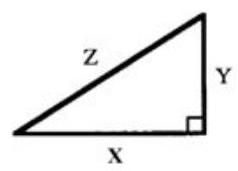
\includegraphics[max width=0.2\textwidth]{images/bo_d3lj80c601uc738kffi0_16_718_1301_238_171_0.jpg}
\end{center}

每个古埃及人都知道，(3,4,5)和(5,12,13)是勾股数.问题是如何找到所有整数解？该方程是齐次的，因此令\(x = X/Z,y = Y/Z\)，它对应着圆\(C : \left( {{x}^{2} + {y}^{2} = 1}\right)  \subset  {\mathbb{R}}^{2}\) ，可以被参数化为

\[
x = \frac{2\lambda }{{\lambda }^{2} + 1},\;y = \frac{{\lambda }^{2} - 1}{{\lambda }^{2} + 1},\;\text{其中}\;\lambda  = \frac{x}{1 - y};
\]

由此可得通解:

\[
X = 2\ell m,\;Y = {\ell }^{2} - {m}^{2},\;Z = {\ell }^{2} + {m}^{2}\;\text{其中}\ell ,m \in  \mathbb{Z}\text{互素}
\]

(如果 \(\ell ,m\) 均为奇数，则各除以2).注意该方程是齐次的，因此如果(X, Y, Z)是解，则 \(\left( {{\lambda X},{\lambda Y},{\lambda Z}}\right)\) 也是解.

也许这个参数化在学校几何中已经熟悉，无论如何，很容易验证它是正确的.然而，如果我之前不知道它，我可以通过一个简单的几何论证得到它，即从给定点的线性射影: \(P = \left( {0,1}\right)  \in  C\) ，如果 \(\lambda  \in  \mathbb{Q}\)
\begin{center}
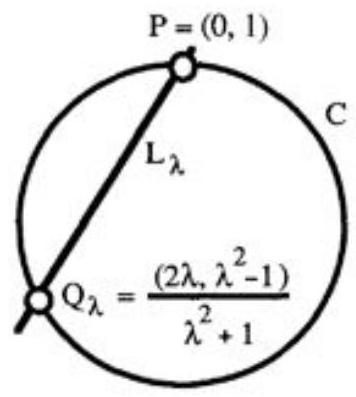
\includegraphics[max width=0.2\textwidth]{images/bo_d3lj80c601uc738kffi0_17_772_501_356_397_0.jpg}
\captionof{figure}{圆锥曲线到直线的线性射影}
\end{center}

是任意值，则通过 \(P\) 且斜率为 \(- \lambda\) 的直线 \({L}_{\lambda }\) 与 \(C\) 相交于另一点 \({Q}_{\lambda }\) .这种通过线性射影构造映射的方法将在后续多次出现.

\section{类似例子}

\(C : \left( {2{X}^{2} + {Y}^{2} = 5{Z}^{2}}\right)\) .同样的方法导出了参数化 \(\mathbb{R} \rightarrow  C\) ，其表达式为

\[
x = \frac{2\sqrt{5}\lambda }{1 + 2{\lambda }^{2}},\;y = \frac{2{\lambda }^{2} - 1}{1 + 2{\lambda }^{2}}.
\]

这使我们能够理解所有系数属于 \(\mathbb{R}\) 的 \(C\) 上的点，且与前一个例子没有实质区别；那么 \(\mathbb{Q}\) 呢？

命题 如果 \(\left( {a,b,c}\right)  \in  \mathbb{Q}\) 满足 \(2{a}^{2} + {b}^{2} = 5{c}^{2}\) ，则 \(\left( {a,b,c}\right)  = \left( {0,0,0}\right)\) .

证明 通过乘以公分母并在必要时提取公因子，我可以假设 \(a,b,c\) 是整数，且不全被5整除；此外，如果 \(5 \mid  a\) 且 \(5 \mid  b\) ，则 \({25} \mid  5{c}^{2}\) ，从而 \(5 \mid  c\) ，这与我刚才所说矛盾.现在通过考虑 \(a\) 和 \(b{\;\operatorname{mod}\;5}\) 的可能取值很容易得到矛盾:由于任何平方数都是0、1或4 \({\;\operatorname{mod}\;5}\) ，显然 \(2{a}^{2} + {b}^{2}\) 是 \(0 + 1,0 + 4,2 + 0,2 + 1,2 + 4,8 + 0,8 + 1\) 或 \(8 + 4{\;\operatorname{mod}\;5}\) 之一，且都不可能是 \(5{c}^{2}\) 的形式.证毕.

注意这是一个彻底的算术论证.

\section{\({\mathbb{R}}^{2}\) 中的圆锥曲线}

\({\mathbb{R}}^{2}\) 中的圆锥曲线是由二次方程给出的平面曲线
\[
q\left( {x,y}\right)  = a{x}^{2} + {bxy} + c{y}^{2} + {dx} + {ey} + f = 0.
\]

每个人都见过非退化圆锥曲线的分类:

\begin{center}
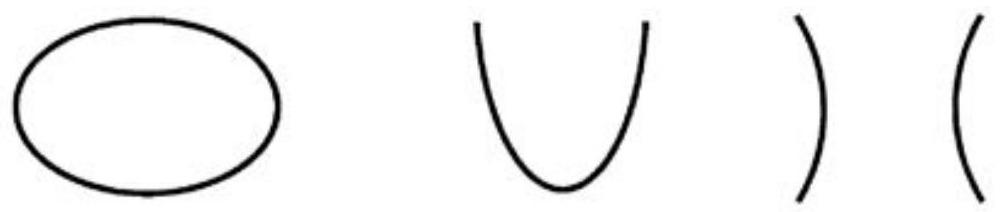
\includegraphics[max width=0.7\textwidth]{images/bo_d3lj80c601uc738kffi0_18_341_562_1004_212_0.jpg}
\captionof{figure}{非退化圆锥曲线:(a) 椭圆；(b) 抛物线；(c) 双曲线.}
\end{center}
\hspace*{3em} 


此外，还有一些特殊情况:

(d) 由 \({x}^{2} + {y}^{2} = 0\) 给出的单点；

(e, f, g) 由以下三个方程中的任意一个给出的空集:(e) \({x}^{2} + {y}^{2} =  - 1\) ，(f) \({x}^{2} =  - 1\) 或 (g) \(0 = 1\) .这三个方程不同，尽管它们在 \({\mathbb{R}}^{2}\) 中定义了相同的零点轨迹；例如考虑它们的复数解.

(h) 直线 \(x = 0\) ；

(i) 直线对 \({xy} = 0\) ；

(j) 平行直线 \(x\left( {x - 1}\right)  = 0\) ；

(k) “重直线” \({x}^{2} = 0\) ；你可以自行决定是否允许最后一种情况:

(l) 由 \(0 = 0\) 给出的整个平面.

\section{射影平面}

“凭空”定义:

\begin{align*}
{\mathbb{P}}^{2}\mathbb{R} &= \left\{{\mathbb{R}}^{3}\text{中经过原点的直线}\right\}\\
&= \{ \text{比例}X : Y : Z\}\\
&= \left( {{\mathbb{R}}^{3}\setminus \{ 0\} }\right) / \sim  ,\;\text{其中}\left( {X,Y,Z}\right)  \sim  \left( {{\lambda X},{\lambda Y},{\lambda Z}}\right),\forall\,\lambda  \in  \mathbb{R} \setminus  \{ 0\} .
\end{align*}

(有经验的读者将轻松地从 \({\mathbb{R}}^{3}\) 推广到任意域上的向量空间，并用内在论证替代选定坐标系中的计算.)

为了表示比值 \(X : Y : Z\) ，其中 \(Z \neq  0\) ，我可以设定 \(x = X/Z,y = Y/Z\) ；这简化了问题，因为该比值对应于仅两个实数.换言之，(X, Y, Z)在 \(\sim\) 下的等价类有唯一代表(x, y,1)，其第三坐标为 \(= 1\) .不幸的是，有时 \(Z\) 可能为 \(= 0\) ，因此这种选择等价类代表的方法就不适用了.这说明 \({\mathbb{P}}^{2}\mathbb{R}\) 包含了 \({\mathbb{R}}^{2}\) 的一个副本.示意图:

\begin{center}
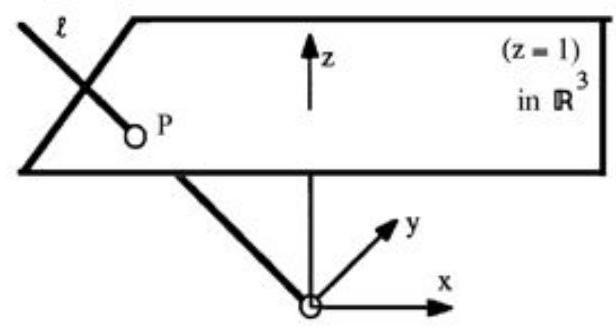
\includegraphics[max width=0.4\textwidth]{images/bo_d3lj80c601uc738kffi0_19_646_280_616_328_0.jpg}
\captionof{figure}{由 \({\mathbb{R}}^{2} \hookrightarrow  {\mathbb{R}}^{3} \setminus  \{ 0\}  \rightarrow  {\mathbb{P}}^{2}\mathbb{R}\) 除以 \(\left( {x,y}\right)  \mapsto  \left( {x,y,1}\right)\)}
\end{center}
\hspace*{3em} 

\({\mathbb{R}}^{3}\) 中通过0的一般直线不包含于平面 \(\left( {Z = 0}\right)\) ，因此它与 \(\left( {Z = 1}\right)\) 恰好相交于一点，该点是该等价类的代表. \(\left( {Z = 0}\right)\) 中的直线永远不与 \(\left( {Z = 1}\right)\) 相交，因此它们对应的不是 \({\mathbb{R}}^{2}\) 的点，而是渐近方向，或 \({\mathbb{R}}^{2}\) 中平行直线簇；所以你可以将 \({\mathbb{P}}^{2}\mathbb{R}\) 视为由 \({\mathbb{R}}^{2}\) 及每个平行直线簇的一个“无穷远点”组成.从这个角度看，你在 \({\mathbb{R}}^{2}\) 中计算，试图通过某种“渐近”论证猜测无穷远处的情况，然后(如有必要)用齐次坐标证明.用 \({\mathbb{R}}^{3}\) 中的直线定义使这一点合理，因为它平等对待了 \({\mathbb{P}}^{2}\mathbb{R}\) 中的所有点.

变换群在整个几何学中具有核心重要性；几何图形的性质必须在适当类型的变换下保持不变，才能具有意义. \({\mathbb{R}}^{2}\) 中的仿射坐标变换形式为 \(T\left( z\right)  = Ax + B\) ，其中 \(x = \left( {x,y}\right)  \in  {\mathbb{R}}^{2}\) ， \(A\) 是一个 \(2 \times  2\) 可逆矩阵， \(B\) 是平移向量；如果 \(A\) 是正交矩阵，则该变换 \(T\) 是欧氏变换.众所周知，每个非退化的圆锥曲线都可以通过欧氏变换化简为上述标准形式(a-c)之一.读者可以尝试证明，每个圆锥曲线都可以通过仿射变换化简为形式(a-1)之一.

\({\mathbb{P}}^{2}\mathbb{R}\) 的射影变换或射影映射是形如 \(T\left( \mathbf{X}\right)  = M\mathbf{X}\) 的映射，其中 \(M\) 是一个可逆的 \(3 \times  3\) 矩阵.理解该变换对仿射部分 \({\mathbb{R}}^{2} \subset  {\mathbb{P}}^{2}\mathbb{R}\) 的作用很简单:作为一个部分定义的映射 \({\mathbb{R}}^{2} \rightarrow  {\mathbb{R}}^{2}\) ，它是分式线性变换.

\[
\left( \begin{array}{l} x \\  y \end{array}\right)  \mapsto  \left( {A\left( \begin{array}{l} x \\  y \end{array}\right)  + B}\right) /\left( {{cx} + {dy} + e}\right) ,\;\text{ where }\;M = \left( \begin{matrix} A & B \\  c & d \end{matrix}\right) .
\]

当 \({cx} + {dy} + e = 0\) 时， \(T\) 当然未定义.或许这看起来不太直观，但它确实存在于自然界:同一(平面)物体的两张不同照片显然通过射影变换相关；参见例如[Berger, 4.7.4]中的图片.因此，一位数学研究生若从事卫星摄影解译工作(无论是为林业委员会的和平目的，还是作为里根总统国防政策带来的广阔职业前景的一部分)，将花费大量时间计算射影变换.

射影变换在这些笔记中隐含使用，通常以“通过适当选择坐标，我可以假设……”的形式出现.

\section{圆锥曲线的方程}

非齐次二次多项式

\[
q\left( {x,y}\right)  = a{x}^{2} + {bxy} + c{y}^{2} + {dx} + {ey} + f
\]

对应于齐次二次多项式

\[
Q\left( {X,Y,Z}\right)  = a{X}^{2} + {bXY} + c{Y}^{2} + {dXZ} + {eYZ} + f{Z}^{2};
\]

这种对应关系易于理解为一种操作步骤，或者你也可以将其视为由 \(q \leftrightarrow  Q\) 给出的双射

\[
q\left( {x,y}\right)  = Q\left( {X/Z,Y/Z,1}\right) \;\text{ with }\;x = X/Z,y = Y/Z
\]

反之亦然，

\[
Q = {Z}^{2}q\left( {X/Z,Y/Z}\right) .
\]

圆锥曲线 \(C \subset  {\mathbb{P}}^{2}\) 是由 \(C : \left( {Q\left( {X,Y,Z}\right)  = 0}\right)\) 给出的曲线，其中 \(Q\) 是一个齐次二次表达式；注意条件 \(Q\left( {X,Y,Z}\right)  = 0\) 在等价类上定义良好，因为对于任意 \(\lambda  \in  \mathbb{R}\) ，有 \(Q\left( {\lambda \mathbf{X}}\right)  = {\lambda }^{2}Q\left( \mathbf{X}\right)\) .作为练习，验证射影曲线 \(C\) 在仿射片 \({\mathbb{R}}^{2}\) 中与由 \(\left( {q = 0}\right)\) 给出的仿射圆锥曲线相交.

\subsection{“无穷远直线”与渐近方向}

\({\mathbb{P}}^{2}\) 中满足 \(Z = 0\) 的点对应于比值 \(\left( {X : Y : 0}\right)\) .这些点构成无穷远直线，是 \({\mathbb{P}}_{\mathbb{R}}^{1} = \mathbb{R} \cup  \{ \infty \}\) 的一个副本(因为 \(\left( {X : Y}\right)  \mapsto  X/Y\) 定义了一个从 \({\mathbb{P}}_{\mathbb{R}}^{1} \rightarrow  \mathbb{R} \cup  \{ \infty \}\) 到 \({\mathbb{P}}_{\mathbb{R}}^{1} = \mathbb{R} \cup  \{ \infty \}\) 的双射).

\({\mathbb{P}}^{2}\) 中的直线定义为由 \(L : \left( {{aX} + {bY} + {cZ} = 0}\right)\) 给出，且

\[
L\text{ passes through }\left( {X,Y,0}\right)  \Leftrightarrow  {aX} + {bY} = 0\text{ . }
\]

在仿射坐标中，同一条直线由 \({ax} + {by} + c = 0\) 给出，因此所有具有相同比例 \(a : b\) 的直线都通过同一个无穷远点.这称为“平行线在无穷远处相交”.

例(a) 双曲线 \(\left( {\frac{{x}^{2}}{{a}^{2}} - \frac{{y}^{2}}{{b}^{2}} = 1}\right)\) 在 \({\mathbb{R}}^{2}\) 中对应于 \({\mathbb{P}}^{2}\mathbb{R}\) 中的 \(C : \left( {\frac{{X}^{2}}{{a}^{2}} - \frac{{Y}^{2}}{{b}^{2}} = {Z}^{2}}\right)\) ；显然它在 \(\left( {Z = 0}\right)\) 中与两点 \(\left( {a, \pm  b,0}\right)  \in  {\mathbb{P}}^{2}\mathbb{R}\) 相交，这两点显然对应于双曲线的渐近线.

注意，在 \({\mathbb{P}}^{2}\mathbb{R}\) 的仿射片 \(\left( {X \neq  0}\right)\) 中，仿射坐标为 \(u = Y/X,v = Z/X\) ，因此 \(C\) 变为椭圆 \(\left( {\frac{{u}^{2}}{{b}^{2}} + {v}^{2} = \frac{1}{{a}^{2}}}\right)\) .参见练习1.7中的艺术性诠释.

(b) 抛物线 \(\left( {y = m{x}^{2}}\right)\) 在 \({\mathbb{R}}^{2}\) 中对应于 \({\mathbb{P}}^{2}\mathbb{R}\) 中的 \(C : \left( {{YZ} = m{X}^{2}}\right)\) ；它现在在单点(0,1,0)处与 \(\left( {Z = 0}\right)\) 相交.因此在 \({\mathbb{P}}^{2}\) 中，“抛物线的两支在无穷远处相遇”；注意这是一条具有直观意义的陈述(也许你觉得这很难以置信？)，但这不是仅凭在 \({\mathbb{R}}^{2} -\) 内的思考就能得出的结论，甚至可能没有意义.

\section{\({\mathbb{P}}^{2}\) 中圆锥曲线的分类}

设 \(k\) 为特征为 \(\neq  2\) 的任意域；回顾二次型线性代数中的两个结果:

命题 (A) 存在自然的双射

\[
\left\{  \begin{matrix} \text{ homogeneous } \\  \text{ quadratic polys. } \end{matrix}\right\}   = \left\{  \begin{matrix} \text{ quad. forms } \\  {k}^{3} \rightarrow  k \end{matrix}\right\}  \overset{\text{ bij }}{ \leftrightarrow  }\left\{  \begin{matrix} \text{ symmetric bilinear } \\  \text{ forms on }{k}^{3} \end{matrix}\right\}
\]

由公式给出

\[
a{X}^{2} + {2bXY} + c{Y}^{2} + {2dXZ} + {2eYZ} + f{Z}^{2} \leftrightarrow  \left( \begin{array}{lll} a & b & d \\  b & c & e \\  d & e & f \end{array}\right)
\]

当对应的双线性型非退化，即其矩阵非奇异时，二次型称为非退化的.

定理 (B) 设 \(V\) 为定义在 \(k\) 上的向量空间， \(Q : V \rightarrow  k\) 为二次型；则存在 \(V\) 的一组基，使得

\[
Q = {\varepsilon }_{1}{x}_{1}^{2} + {\varepsilon }_{2}{x}_{2}^{2} + \cdots  + {\varepsilon }_{n}{x}_{n}^{2},\text{ with }{\varepsilon }_{i} \in  k.
\]

(这通过Gram-Schmidt正交化法证明，如果你还记得的话.)显然，对于 \(\lambda  \in\)  \(k \setminus  \{ 0\}\) ，代换 \({x}_{i} \mapsto  \lambda {x}_{i}\) 将 \({\varepsilon }_{i}\) 变为 \({\lambda }^{-2}{\varepsilon }_{i}\) .

推论 在适当的坐标系中， \({\mathbb{P}}^{2}\mathbb{R}\) 中的任一圆锥曲线为以下之一:

( \(\alpha\) )非退化圆锥曲线， \(C : \left( {{X}^{2} + {Y}^{2} - {Z}^{2} = 0}\right)\) ；

( \(\beta\) )空集，由 \(\left( {{X}^{2} + {Y}^{2} + {Z}^{2} = 0}\right)\) 给出；

(γ)直线对，由 \(\left( {{X}^{2} - {Y}^{2} = 0}\right)\) 给出；

(δ)单点(0,0,1)，由 \(\left( {{X}^{2} + {Y}^{2} = 0}\right)\) 给出；

(ε)重直线，由 \(\left( {{X}^{2} = 0}\right)\) 给出.

(可选地，整个 \({\mathbb{P}}^{2}\mathbb{R}\) 由 \(\left( {0 = 0}\right)\) 给出.)

证明 任意实数 \(\varepsilon\) 要么为0，要么为±平方数，因此我只需考虑定理中 \(Q\) 为 \({\varepsilon }_{i} = 0\) 或 \(\pm  1\) 的情况.此外，由于我只关心轨迹 \(\left( {Q = 0}\right)\) ，允许将 \(Q\) 乘以-1.这立即导出上述列表.证毕.

关于此推论有两点需要说明:首先，该列表比(1.3)中的要短得多；例如，(1.3)中的3种非退化情况(椭圆、抛物线、双曲线)均对应于 \(\left( \alpha \right)\) 情况，而相交和平行直线对在射影情况下未加区分.其次，该列表从一般代数原理推导出来更为简洁.

\section{1.7 圆锥曲线的参数化}

设 \(C\) 为 \({\mathbb{P}}^{2}\mathbb{R}\) 中一个非退化且非空的圆锥曲线.则根据推论1.6，取新坐标后， \(\left( {X + Z,Y,Z - X}\right) ,C\) 与曲线 \(\left( {{XZ} = {Y}^{2}}\right)\) 在射影意义下等价；该曲线由下式参数化

\[
\Phi  : {\mathbb{P}}_{\mathbb{R}}^{1} \rightarrow  C \subset  {\mathbb{P}}^{2}\mathbb{R}
\]

\[
\left( {U : V}\right)  \mapsto  \left( {{U}^{2} : {UV} : {V}^{2}}\right) .
\]

备注1 逆映射 \(\Psi  : C \rightarrow  {\mathbb{P}}_{\mathbb{R}}^{1}\) 由下式给出

\[
\left( {X : Y : Z}\right)  \mapsto  \left( {X : Y}\right)  = \left( {Y : Z}\right) ;
\]

此处左侧的比值在 \(X \neq  0\) 时定义，右侧的比值在 \(Z \neq  0\) 时定义.用稍后引入的术语， \(\Phi\) 和 \(\Psi\) 是簇的逆同构.

2 在整个 \(§§1 - 2\) 中，默认非空非退化圆锥曲线在射影意义下等价于 \(\left( {{XZ} - {Y}^{2}}\right)\) ；在特征为 \(\neq  2\) 的域上，这一点在练习1.5中得到了证明.(对特征2感兴趣的读者应将此作为非退化圆锥曲线的定义.)

\section{1.8 两变量齐次形式}

设 \(F\left( {U,V}\right)\) 为 \(U,V\) 中一个次数为 \(d\) 的非零齐次多项式，系数属于固定域 \(k\) ；(我将沿用传统，使用“形式”一词表示“齐次多项式”):

\[
F\left( {U,V}\right)  = {a}_{d}{U}^{d} + {a}_{d - 1}{U}^{d - 1}V + \cdots  + {a}_{i}{U}^{i}{V}^{d - i} + \cdots  + {a}_{0}{V}^{d}.
\]

\(F\) 对应一个一元非齐次多项式，

\[
f\left( u\right)  = {a}_{d}{u}^{d} + {a}_{d - 1}{u}^{d - 1} + \cdots  + {a}_{i}{u}^{i} + \cdots  + {a}_{0}.
\]

显然对于 \(\alpha  \in  k\) ，

\[
f\left( \alpha \right)  = 0 \Leftrightarrow  \left( {u - \alpha }\right)  \mid  f\left( u\right)
\]

\[
\Leftrightarrow  \left( {U - {\alpha V}}\right)  \mid  F\left( {U,V}\right)  \Leftrightarrow  F\left( {\alpha ,1}\right)  = 0;
\]

因此 \(f\) 的零点对应于 \({\mathbb{P}}^{1}\) 上除点(1,0)——即“点 \(\alpha  = \infty\) ”外的 \(F\) 的零点. \(F\) 在无穷远点有零点意味着什么？

\[
F\left( {1,0}\right)  = 0 \Leftrightarrow  {a}_{d} = 0 \Leftrightarrow  \deg f < d.
\]

现定义 \(F\) 在 \({\mathbb{P}}^{1}\) 上的零点的重数为

(i) 对应于 \(\alpha  \in  k\) 处 \(f\) 的重数；或

(ii) 若零点为(1,0)，则为 \(d - \deg f\) .

因此， \(F\) 在点 \(\left( {\alpha ,1}\right)\) 处的零点重数是整除 \(F\) 的最大 \(\left( {U - {\alpha V}}\right)\) 次幂，而在(1,0)处则是整除 \(F\) 的最大 \(V\) 次幂.

命题 设 \(F\left( {U,V}\right)\) 为 \(U,V\) 中次数为 \(d\) 的非零形式.则 \(F\) 在 \({\mathbb{P}}^{1}\) 上最多有 \(d\) 个零点；此外，若 \(k\) 是代数闭域，则 \(F\) 在 \({\mathbb{P}}^{1}\) 上恰有 \(d\) 个零点，前提是这些零点按上述定义的重数计数.

证明 设 \({m}_{\infty }\) 为 \(F\) 在(1,0)处零点的重数；则根据定义， \(d - {m}_{\infty }\) 是非齐次多项式 \(f\) 的次数，命题归结为一元多项式最多有 \(\deg f\) 个根的众所周知的事实.证毕.

注意，在代数闭域上， \(F\) 可分解为线性形式 \({\lambda }_{i} = \left( {{a}_{i}U + {b}_{i}V}\right)\) 的乘积 \(F = \prod {\lambda }_{i}^{{m}_{i}}\) ，以此方式处理时，点(1,0)对应形式 \({\lambda }_{\infty } = V\) ，与其他点处于同等地位.

\section{Bézout定理的简单情形}

Bézout定理指出，如果 \(C\) 和 \(D\) 是次数分别为 \(\deg C = m,\deg D = n\) 的平面曲线，那么它们的交点数为 \({mn}\) ，前提是(i)域是代数闭合的；(ii)交点按正确的重数计数；(iii)我们在 \({\mathbb{P}}^{2}\) 中工作，以正确考虑“无穷远处”的交点.详见例如[Fulton，第112页]的自包含证明.本节将讨论其中一条曲线为直线或圆锥曲线的情况.

定理 设 \(L \subset  {\mathbb{P}}_{k}^{2}\) 为一条直线(分别为 \(C \subset  {\mathbb{P}}_{k}^{2}\) 一条非退化圆锥曲线)，且设 \(D \subset  {\mathbb{P}}_{k}^{2}\) 为由 \(D : \left( {{G}_{d}\left( {X,Y,Z}\right)  = 0}\right)\) 定义的曲线，其中 \(G\) 是 \(X,Y,Z\) 中次数为 \(d\) 的齐次多项式.假设 \(L ⊄ D\) (分别为 \(C ⊄ D\) )；则

\[
\# \{ L \cap  D\}  \leq  d\;\text{ (respectively }\# \{ C \cap  D\}  \leq  {2d}\text{ ). }
\]

事实上，存在一个自然的交点重数定义，使得不等式对“按重数计数的点数”仍然成立，且如果 \(k\) 是代数闭合的，则等号成立.

证明 一条直线 \(L \subset  {\mathbb{P}}_{k}^{2}\) 由方程 \(\lambda  = 0\) 给出，其中 \(\lambda\) 是线性形式；为方便起见，我用参数形式表示为

\[
X = a\left( {U,V}\right) ,\;Y = b\left( {U,V}\right) ,\;Z = c\left( {U,V}\right) ,
\]

其中 \(a,b,c\) 是 \(U,V\) 中的线性形式.例如，如果 \(\lambda  = {\alpha X} + {\beta Y} + {\gamma Z}\) ，且 \(\gamma  \neq  0\) ，则 \(L\) 可以

表示为

\[
X = U,\;Y = V,\;Z =  - \frac{\alpha }{\gamma }U - \frac{\beta }{\gamma }V.
\]

类似地，如(1.7)所述，非退化圆锥曲线可以参数化表示为

\[
X = a\left( {U,V}\right) ,\;Y = b\left( {U,V}\right) ,\;Z = c\left( {U,V}\right) ,
\]

其中 \(a,b,c\) 是 \(U,V\) 中的二次形式.这是因为 \(C\) 是 \(\left( {{XZ} = {Y}^{2}}\right)\) 的射影变换，而 \(\left( {{XZ} = {Y}^{2}}\right)\) 的参数形式为 \(\left( {X,Y,Z}\right)  = \left( {{U}^{2},{UV},{V}^{2}}\right)\) ，因此 \(C\) 由下式给出

\[
\left( \begin{array}{l} X \\  Y \\  Z \end{array}\right)  = M\left( \begin{matrix} {U}^{2} \\  {UV} \\  {V}^{2} \end{matrix}\right)
\]

其中 \(M\) 是一个非奇异的 \(3 \times  3\) 矩阵.

\begin{center}
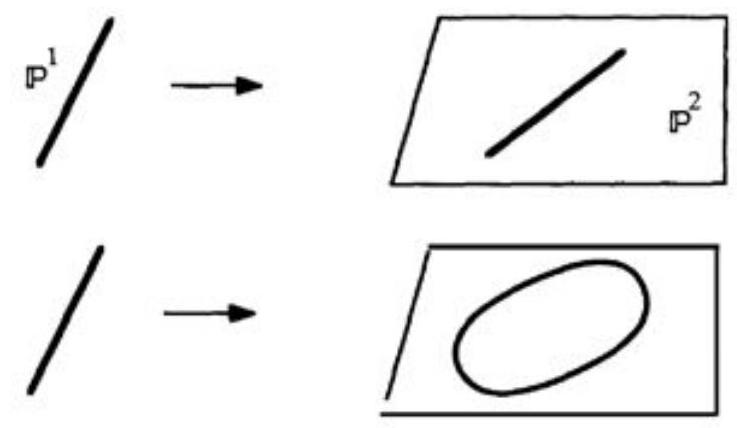
\includegraphics[max width=0.5\textwidth]{images/bo_d3lj80c601uc738kffi0_24_454_273_737_428_0.jpg}
\end{center}
\hspace*{3em} 

图1.4:(a)参数化直线；(b)参数化圆锥曲线

那么 \(L\) (分别为 \(C\) )与 \(D\) 的交点由求解比值 \(\left( {U : V}\right)\) 的值确定，使得

\[
F\left( {U,V}\right)  = {G}_{d}\left( {a\left( {U,V}\right) ,b\left( {U,V}\right) ,c\left( {U,V}\right) }\right)  = 0.
\]

但 \(F\) 是 \(U,V\) 中次数为 \(d\) (分别为 \({2d}\) )的齐次多项式，故结果由(1.8)得出.证毕.

\setboxcounter{corollary}{9}
\begin{corollary}\label{cor:1.10}
    若 \({P}_{1},\ldots ,{P}_{5} \in  {\mathbb{P}}^{2}\mathbb{R}\) 为不同点且无四点共线，则最多存在一条经过 \({P}_{1},\ldots ,{P}_{5}\) 的圆锥曲线.ss
\end{corollary}

\begin{proof}
    反设 \({C}_{1}\) 和 \({C}_{2}\) 为圆锥曲线，且 \({C}_{1} \neq  {C}_{2}\) 使得

\[
{C}_{1} \cap  {C}_{2} \supset  \left\{  {{P}_{1},\ldots ,{P}_{5}}\right\}
\]

\({C}_{1}\) 非空，则若其非退化，则由(1.7)知其在射影意义下等价于参数化曲线

\[
{C}_{1} = \left\{  {\left( {{U}^{2},{UV},{V}^{2}}\right)  \mid  \left( {U,V}\right)  \in  {\mathbb{P}}^{1}}\right\}  ;
\]
由 \(\left( {1.9}\right) ,{C}_{1} \subset  {C}_{2}\) .现在如果 \({Q}_{2}\) 是 \({C}_{2}\) 的方程，则对于所有 \(\left( {U,V}\right)  \in  {\mathbb{P}}^{1}\) 都有 \({Q}_{2}\left( {{U}^{2},{UV},{V}^{2}}\right)  \equiv  0\) ，且一个简单的计算(见练习1.6)表明 \({Q}_{2}\) 是 \(\left( {{XZ} - {Y}^{2}}\right)\) 的倍数；这与 \({C}_{1} \neq  {C}_{2}\) 矛盾.

现在假设 \({C}_{1}\) 是退化的；根据(1.6)，它要么是一对直线，要么是一条直线，很容易看出

\[
{C}_{1} = {L}_{0} \cup  {L}_{1},\;{C}_{2} = {L}_{0} \cup  {L}_{2},
\]

其中 \({L}_{1},{L}_{2}\) 是不同的直线.则 \({C}_{1} \cap  {C}_{2} = {L}_{0} \cup  \left( {{L}_{1} \cap  {L}_{2}}\right)\) :

\begin{center}
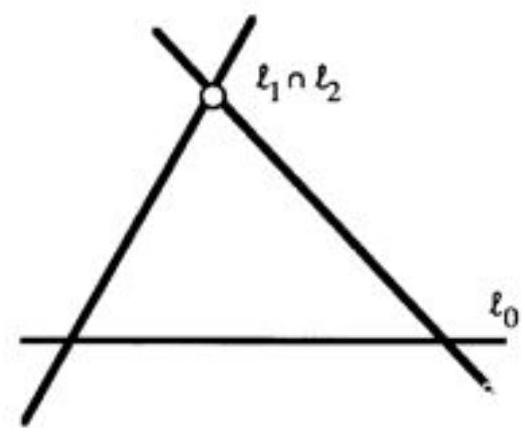
\includegraphics[max width=0.4\textwidth]{images/bo_d3lj80c601uc738kffi0_25_718_284_525_437_0.jpg}
\captionof{figure}{相交的直线}
\end{center}
\hspace*{3em} 



因此 \({P}_{1},\ldots ,{P}_{5}\) 中的4个点位于 \({L}_{0}\) 上，矛盾.
\end{proof}


\setcounter{section}{10}
\section{所有圆锥曲线的空间}

设

\[
{S}_{2} = \left\{  {\text{ quadratic forms on }{\mathbb{R}}^{3}}\right\}   = \{ 3 \times  3\text{ symmetric matrixes }\}  \cong  {\mathbb{R}}^{6}.
\]

如果 \(Q \in  {S}_{2}\) ，写作 \(Q = a{X}^{2} + {2bXY} + \cdots  + f{Z}^{2}\) ；对于 \({P}_{0} = \left( {{X}_{0},{Y}_{0},{Z}_{0}}\right)  \in  {\mathbb{P}}^{2}\mathbb{R}\) ，考虑关系 \({P}_{0} \in  C : \left( {Q = 0}\right)\) .这具有以下形式

\[
Q\left( {{X}_{0},{Y}_{0},{Z}_{0}}\right)  = a{X}_{0}^{2} + {2b}{X}_{0}{Y}_{0} + \cdots  + f{Z}_{0}^{2} = 0,
\]

对于固定的 \({P}_{0}\) ，这是关于 \(\left( {a,b,\ldots ,f}\right)\) 的线性方程.因此

\[
{S}_{2}\left( {P}_{0}\right)  = \left\{  {Q \in  {S}_{2} \mid  Q\left( {P}_{0}\right)  = 0}\right\}   \cong  {\mathbb{R}}^{5} \subset  {S}_{2} = {\mathbb{R}}^{6}
\]

是一个5维超平面.对于 \({P}_{1},\ldots ,{P}_{n} \in  {\mathbb{P}}^{2}\mathbb{R}\) ，类似定义

\[
{S}_{2}\left( {{P}_{1},\ldots ,{P}_{n}}\right)  = \left\{  {Q \in  {S}_{2} \mid  Q\left( {P}_{i}\right)  = 0\text{ for }i = 1,\ldots ,n}\right\}  ;
\]

则在 \(Q\) 的6个系数 \(\left( {a,b,\ldots ,f}\right)\) 中有 \(n\) 个线性方程.由此得到结果:

命题 \(\dim {S}_{2}\left( {{P}_{1},\ldots ,{P}_{n}}\right)  \geq  6 - n\) .

我们还可以预期“当 \({P}_{1},\ldots ,{P}_{n}\) 足够一般时等号成立”.更准确地说:

推论 如果 \(n \leq  5\) 且 \({P}_{1},\ldots ,{P}_{n}\) 中没有4点共线，则

\[
\dim {S}_{2}\left( {{P}_{1},\ldots ,{P}_{n}}\right)  = 6 - n.
\]

证明 推论1.10表明如果 \(n = 5\) ，则 \(\dim {S}_{2}\left( {{P}_{1},\ldots ,{P}_{5}}\right)  \leq  1\) ，这在此情况下给出推论.如果 \(n \leq  4\) ，则我可以加入点 \({P}_{n + 1},\ldots ,{P}_{5}\) ，同时保持没有4点共线的条件，且由于每个点最多施加一个线性条件，这给出

\[
1 = \dim {S}_{2}\left( {{P}_{1},\ldots ,{P}_{5}}\right)  \geq  \dim {S}_{2}\left( {{P}_{1},\ldots ,{P}_{n}}\right)  - \left( {5 - n}\right) \text{ . Q.E.D. }
\]

注意，如果给定6个点 \({P}_{1},\ldots ,{P}_{6} \in  {\mathbb{P}}^{2}\mathbb{R}\) ，它们可能在圆锥曲线上，也可能不在.

\section{1.12 两条圆锥曲线的交点}

如上所述，两条圆锥曲线常常在4个点相交:

\begin{center}
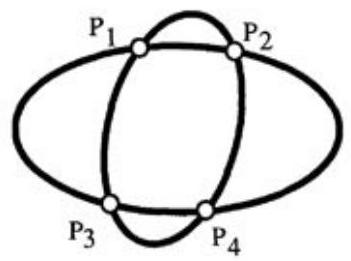
\includegraphics[max width=0.2\textwidth]{images/bo_d3lj80c601uc738kffi0_26_669_694_351_261_0.jpg}
\end{center}
\hspace*{3em} 

反过来，根据推论1.11，给定4个点 \({P}_{1},\ldots ,{P}_{4} \in  {\mathbb{P}}^{2}\) ，在适当条件下 \({S}_{2}\left( {{P}_{1},\ldots ,{P}_{4}}\right)\) 是一个二维向量空间，因此选择 \({S}_{2}\left( {{P}_{1},\ldots ,{P}_{4}}\right)\) 的基 \({Q}_{1},{Q}_{2}\) 会得到两条圆锥曲线 \({C}_{1},{C}_{2}\) ，使得 \({C}_{1} \cap  {C}_{2} = \left\{  {{P}_{1},\ldots ,{P}_{4}}\right\}\) .非奇异圆锥曲线多重交点有多种可能:

\begin{center}
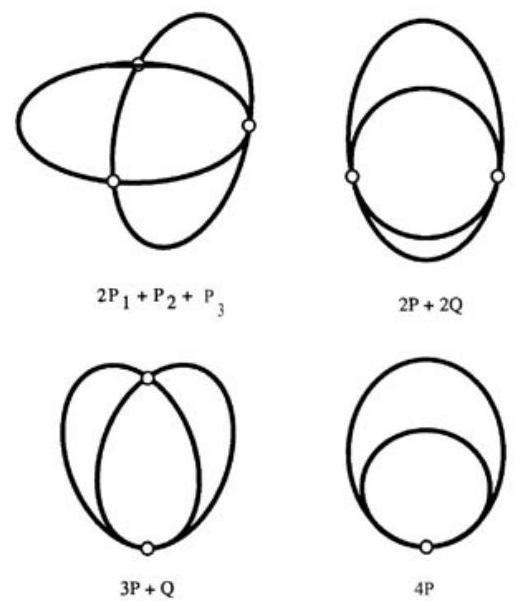
\includegraphics[max width=0.4\textwidth]{images/bo_d3lj80c601uc738kffi0_26_578_1167_519_608_0.jpg}
\end{center}
\hspace*{3em} 

图1.6:(a) \(2{P}_{1} + {P}_{2} + {P}_{3}\) ；(b) \({2P} + {2Q}\) ；(c) \({3P} + Q\) ；(d) \({4P}\)

参见练习1.9获取合适的方程.

\section{1.13 圆锥曲线族中的退化圆锥曲线}

定义 圆锥曲线族(pencil of conics)是形如

\[
{C}_{\left( \lambda ,\mu \right) } : \left( {\lambda {Q}_{1} + \mu {Q}_{2} = 0}\right) ;
\]

的族，每个元素都是平面曲线，线性依赖于参数 \(\left( {\lambda ,\mu }\right)\) ；将比值 \(\left( {\lambda  : \mu }\right)\) 视为 \({\mathbb{P}}^{1}\) 上的一点.

观察示例，可以预期当 \(\left( {\lambda  : \mu }\right)\) 取特殊值时，圆锥曲线 \({C}_{\left( \lambda ,\mu \right) }\) 会退化.事实上，记对应二次型 \(Q\) 的对称矩阵 \(3 \times  3\) 的行列式为 \(\det \left( Q\right)\) ，则显然

\[
{C}_{\left( \lambda ,\mu \right) }\text{ is degenerate } \Leftrightarrow  \det \left( {\lambda {Q}_{1} + \mu {Q}_{2}}\right)  = 0\text{ . }
\]

将 \({Q}_{1}\) 和 \({Q}_{2}\) 写成对称矩阵形式，条件可表达为

\[
F\left( {\lambda ,\mu }\right)  = \det \left| {\lambda \left( \begin{array}{lll} a & b & d \\  b & c & e \\  d & e & f \end{array}\right)  + \mu \left( \begin{array}{lll} {a}^{\prime } & {b}^{\prime } & {d}^{\prime } \\  {b}^{\prime } & {c}^{\prime } & {e}^{\prime } \\  {d}^{\prime } & {e}^{\prime } & {f}^{\prime } \end{array}\right) }\right|  = 0.
\]

注意 \(F\left( {\lambda ,\mu }\right)\) 是关于 \(\lambda ,\mu\) 的齐次三次型.进而我可以对 \(F\) 应用(1.8)推导出:

命题 设 \({C}_{\left( \lambda ,\mu \right) }\) 是 \({\mathbb{P}}_{k}^{2}\) 上的一个圆锥曲线族，且至少包含一个非退化圆锥曲线(即 \(F\left( {\lambda ,\mu }\right)\) 不恒为零).则该族最多有3个退化圆锥曲线.如果 \(k = \mathbb{R}\) ，则该族至少有一个退化圆锥曲线.

证明 三次型有 \(\leq  3\) 个零点.在 \(\mathbb{R}\) 上，它至少有一个零点.

\section{1.14 例题解析}

设 \({P}_{1},\ldots ,{P}_{4}\) 是 \({\mathbb{P}}^{2}\mathbb{R}\) 中的4个点，且无3点共线；则通过 \({P}_{1},\ldots ,{P}_{4}\) 的圆锥曲线族 \({C}_{\left( \lambda ,\mu \right) }\) 有3个退化元素，即线对 \({L}_{12} + {L}_{34},{L}_{13} + {L}_{24},{L}_{14} + {L}_{23}\) ，其中 \({L}_{ij}\) 是通过 \({P}_{i},{P}_{j}\) 的直线:

\begin{center}
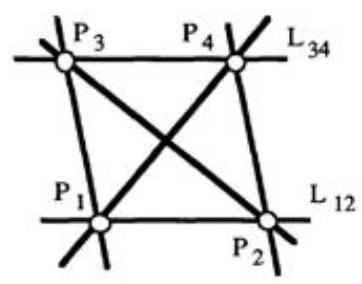
\includegraphics[max width=0.2\textwidth]{images/bo_d3lj80c601uc738kffi0_27_770_1529_362_284_0.jpg}
\end{center}
\hspace*{3em} 

接下来，假设我从由 \({Q}_{1} = {Y}^{2} + {rY} + {sX} + t\) 和 \({Q}_{2} = Y - {X}^{2}\) 生成的圆锥曲线族出发，尝试找到交点 \({P}_{1},\ldots ,{P}_{4}\) .

\begin{center}
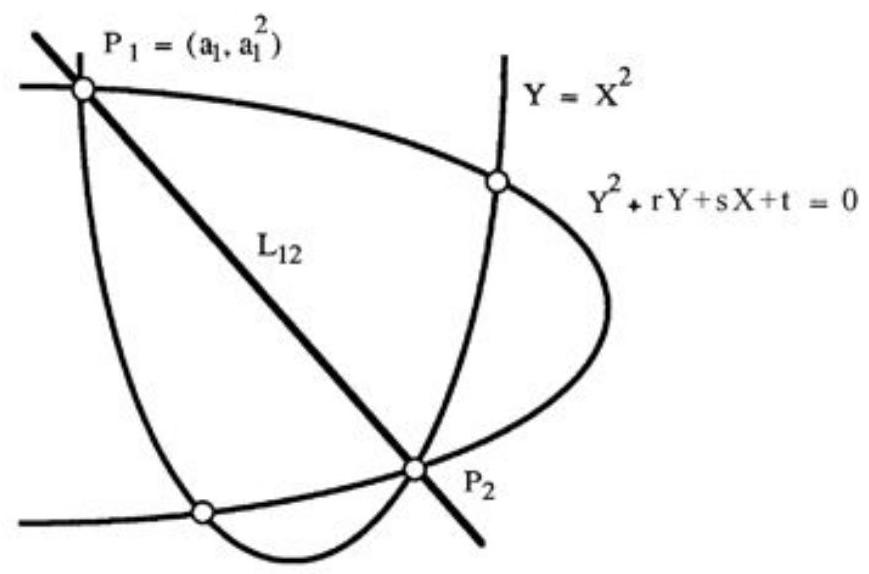
\includegraphics[max width=0.6\textwidth]{images/bo_d3lj80c601uc738kffi0_28_418_286_869_574_0.jpg}
\end{center}
\hspace*{3em} 

这可以按如下方式完成:(1) 找到使 \({C}_{\left( \lambda ,\mu \right) }\) 成为退化圆锥曲线的3个比率 \(\left( {\lambda  : \mu }\right)\) .根据上述内容，这仅意味着我必须找到该三次方程的3个根

\[
F\left( {\lambda ,\mu }\right)  = \det \left| {\lambda \left( \begin{matrix} 0 & 0 & s/2 \\  0 & 1 & r/2 \\  s/2 & r/2 & t \end{matrix}\right)  + \mu \left( \begin{matrix}  - 1 & 0 & 0 \\  0 & 0 & 1/2 \\  0 & 1/2 & 0 \end{matrix}\right) }\right|
\]

\[
=  - \frac{1}{4}\left( {{s}^{2}{\lambda }^{3} + \left( {{4t} - {r}^{2}}\right) {\lambda }^{2}\mu  - {2r\lambda }{\mu }^{2} - {\mu }^{3}}\right) .
\]

(2) 将其中2个退化圆锥曲线分解为直线对(这涉及解2个二次方程).(3) 4个点 \({P}_{i}\) 是这些直线的交点.

该过程为伽罗瓦理论(Galois theory)中一般四次方程的约化提供了几何解释(参见例如[van der Waerden, Algebra, 第8章, \(§{64}\) ]):设 \(k\) 为一个域， \(f\left( X\right)  =\)  \({X}^{4} + r{X}^{2} + {sX} + t \in  k\left\lbrack  X\right\rbrack\) 为一个四次多项式.则两条抛物线 \({C}_{1}\) 和 \({C}_{2}\) 在4个点 \({P}_{i} = \left( {{a}_{i},{a}_{i}^{2}}\right)\) 相交，其中 \(i = 1,\ldots ,4\) ，而 \({a}_{i}\) 是 \(f\) 的4个根.

则直线 \({L}_{ij} = {P}_{i}{P}_{j}\) 由下式给出

\[
{L}_{ij} : \left( {Y = \left( {{a}_{i} + {a}_{j}}\right) X - {a}_{i}{a}_{j}}\right) ,
\]

而可约圆锥曲线 \({L}_{12} + {L}_{34}\) 由下式给出

\[
{Y}^{2} + \left( {{a}_{1}{a}_{2} + {a}_{3}{a}_{4}}\right) Y + \left( {{a}_{1} + {a}_{2}}\right) \left( {{a}_{3} + {a}_{4}}\right) {X}^{2} + {sX} + t = 0,
\]

即由 \({Q}_{1} - \left( {{a}_{1} + {a}_{2}}\right) \left( {{a}_{3} + {a}_{4}}\right) {Q}_{2} = 0\) 给出.因此，使圆锥曲线 \(\lambda {Q}_{1} + \mu {Q}_{2}\) 分解为直线对的3个 \(\mu /\lambda\) 值为

\[
- \left( {{a}_{1} + {a}_{2}}\right) \left( {{a}_{3} + {a}_{4}}\right) ,\; - \left( {{a}_{1} + {a}_{3}}\right) \left( {{a}_{2} + {a}_{4}}\right) ,\; - \left( {{a}_{1} + {a}_{4}}\right) \left( {{a}_{2} + {a}_{3}}\right) .
\]

这些3个量作为根的三次方程称为与四次方程相关的辅助三次方程；它可以通过初等对称函数理论计算；这是一个相当繁琐的过程.另一方面，上述几何方法给出了辅助三次方程的优雅推导，仅涉及计算一个 \(3 \times  3\) 行列式.

上述处理摘自[M.Berger, 16.4.10 和 16.4.11.1].

\section{第一章习题}

1.1 通过考虑经过点(2,1)的变量直线对圆锥曲线 \(C : \left( {{x}^{2} + {y}^{2} = 5}\right)\) 进行参数化，从而求出 \({x}^{2} + {y}^{2} = 5\) 的所有有理解.

1.2 设 \(p\) 为素数；通过对不同的 \(p\) 进行实验，猜测 \({x}^{2} + {y}^{2} = p\) 存在有理解的充要条件；证明你的猜测(提示见下文习题1.9之后

\begin{itemize}
\item 打赌你自己做不到！).
\end{itemize}

1.3 证明(1.3)中的陈述，即仿射变换可用于将任意 \({\mathbb{R}}^{2}\) 的圆锥曲线化为标准形式之一(a-l).【提示:使用线性变换 \(\mathbf{x} \mapsto  A\mathbf{x}\) 将首项 \(a{x}^{2} + {bxy} + c{y}^{2}\) 变换为 \(\pm  {x}^{2} \pm  {y}^{2}\) 或 \(\pm  {x}^{2}\) 或0；然后对 \(x\) 和 \(y\) 完成平方，尽可能消除线性部分.】

1.4 详细比较(1.3)中的仿射圆锥曲线与(1.6)中的射影圆锥曲线.

1.5 设 \(k\) 为特征为 \(\neq  2\) 的任意域， \(V\) 为三维 \(k\) -向量空间；设 \(Q : V \rightarrow  k\) 为 \(V\) 上的非退化二次型.证明若 \(0 \neq  {e}_{1} \in  V\) 满足 \(Q\left( {e}_{1}\right)  = 0\) ，则 \(V\) 存在基 \({e}_{1},{e}_{2},{e}_{3}\) 使得 \(Q\left( {{x}_{1}{e}_{1} + {x}_{2}{e}_{2} + {x}_{3}{e}_{3}}\right)  = {x}_{1}{x}_{3} + a{x}_{2}^{2}\) .【提示:考虑与 \(Q\) 相关的对称双线性型 \(\varphi\) ；由于 \(\varphi\) 非退化，存在向量 \({e}_{3}\) 使得 \(\varphi \left( {{e}_{1},{e}_{3}}\right)  = 1\) .然后找到合适的 \({e}_{2}\) .】

推断非空且非退化的圆锥曲线 \(C \subset  {\mathbb{P}}_{k}^{2}\) 在射影意义下等价于 \(({XZ} =\)  \(\left. {Y}^{2}\right)\) .

1.6 设 \(k\) 为元素数不少于4的域，且 \(C : \left( {{XZ} = {Y}^{2}}\right)  \subset  {\mathbb{P}}_{k}^{2}\) ；证明若 \(Q\left( {X,Y,Z}\right)\) 为在 \(C\) 上消失的二次型，则 \(Q = \lambda \left( {{XZ} - {Y}^{2}}\right)\) .【提示:如果你确实无法自行完成，可参照引理2.5证明中的论证.】

1.7 在 \({\mathbb{R}}^{3}\) 中，考虑两个平面 \(A : \left( {Z = 1}\right)\) 和 \(B : \left( {X = 1}\right)\) ；一条通过0点的直线在 \(A\) 上交于(x, y,1)，在 \(B\) 上交于 \(\left( {1,y/x,1/x}\right)\) .考虑由 \(\left( {x,y}\right)  \mapsto  \left( {y}^{\prime }\right.  =\)  \(\left. {y/x,{z}^{\prime } = 1/x}\right)\) 定义的映射 \(\varphi  : A \rightarrow  B\) ；求 \(\varphi\) 下的像

(i) 直线 \({ax} = y + b\) ；平行线束 \({ax} = y + b\) (固定 \(a\) ，变化 \(b\) )；

(ii) 对于变化的 \(c\) ，圆 \({\left( x - 1\right) }^{2} + {y}^{2} = c\) (区分三种情况 \(c > 1,c = 1\) 和 \(c < 1\) ).

试想象上述内容为一位坐在 \(0 \in  {\mathbb{R}}^{3}\) 上的艺术家，在平面 \(\left( {X = 1}\right)\) 上对平面 \(\left( {Z = 1}\right)\) 上的图形所作的透视画.解释当 \(\varphi\) 和 \({\varphi }^{-1}\) 未定义时，两平面上的点会发生什么变化.

1.8 设 \({P}_{1},\ldots ,{P}_{4}\) 为 \({\mathbb{P}}^{2}\) 中不共线的不同点，且无三点共线.证明存在唯一的坐标系，使得这4点为 \(\left( {1,0,0}\right) ,\left( {0,1,0}\right) ,\left( {0,0,1}\right)\) 和(1,1,1).找出所有经过 \({P}_{1},\ldots ,{P}_{5}\) 的圆锥曲线，其中 \({P}_{5} = \left( {a,b,c}\right)\) 为另一点，并用此给出推论1.10和命题1.11的另一证明.

1.9 在(1.12)中列出了两条圆锥曲线相交的所有可能方式.写出方程证明每种可能确实存在.找出对应线束中所有奇异圆锥曲线.[提示:利用对称性和恰当选择的坐标系可大大简化计算.]

1.2的提示:根据初等数论，-1是模 \(p\) 的二次剩余当且仅当 \(p = 2\) 或 \(p \equiv  1{\;\operatorname{mod}\;4}\) .

1.10(Sylvester行列式).设 \(k\) 为代数闭域，且在 \(U,V\) 中给定二次型和三次型，如(1.8)所示:

\[
q\left( {U,V}\right)  = {a}_{0}{U}^{2} + {a}_{1}{UV} + {a}_{2}{V}^{2},
\]

\[
c\left( {U,V}\right)  = {b}_{0}{U}^{3} + {b}_{1}{U}^{2}V + {b}_{2}U{V}^{2} + {b}_{3}{V}^{3}.
\]

证明 \(q\) 和 \(c\) 有公共零点 \(\left( {\eta  : \tau }\right)  \in  {\mathbb{P}}^{1}\) 当且仅当

\[
\det \left| \begin{array}{lllll} {a}_{0} & {a}_{1} & {a}_{2} & & \\   & {a}_{0} & {a}_{1} & {a}_{2} & \\   & & {a}_{0} & {a}_{1} & {a}_{2} \\  {b}_{0} & {b}_{1} & {b}_{2} & {b}_{3} & \\   & {b}_{0} & {b}_{1} & {b}_{2} & {b}_{3} \end{array}\right|  = 0
\]

[提示:证明若 \(q\) 和 \(c\) 有公共根，则这5个元素

\[
{U}^{2}q,\;{UVq},\;{V}^{2}q,\;{Uc}\;\text{ and }\;{Vc}
\]

不生成4次型的5维向量空间，因此线性相关.反之，利用多项式环 \(k\left\lbrack  {U,V}\right\rbrack\) 中的唯一分解性质，说明形如 \({Aq} = {Bc}\) 的关系，其中 \(A\) 和 \(B\) 为 \(U,V,\deg A = 2,\deg B = 1\) 中的形式.

1.11 将练习1.10的结果推广到 \(U,V\) 中任意次数为 \(n\) 和 \(m\) 的两个形式.

\chapter{三次曲线与群运算律}

\section{参数化三次曲线的例子}

一些平面三次曲线可以像二次曲线一样被参数化：

有结点的三次曲线 \(C: y^2 = x^3 + x^2 \subset \mathbb{R}^2\) 是由映射 \(\varphi: \mathbb{R}^1 \to \mathbb{R}^2\) 给出的像，其表达式为 \(t \mapsto (t^2 - 1, t^3 - t)\)（请自行验证）；

尖点三次曲线 \(C: y^2 = x^3 \subset \mathbb{R}^2\) 是由映射 \(\varphi: \mathbb{R}^1 \to \mathbb{R}^2\) 给出的像，其表达式为 \(t \mapsto (t^2, t^3)\)：

\begin{center}
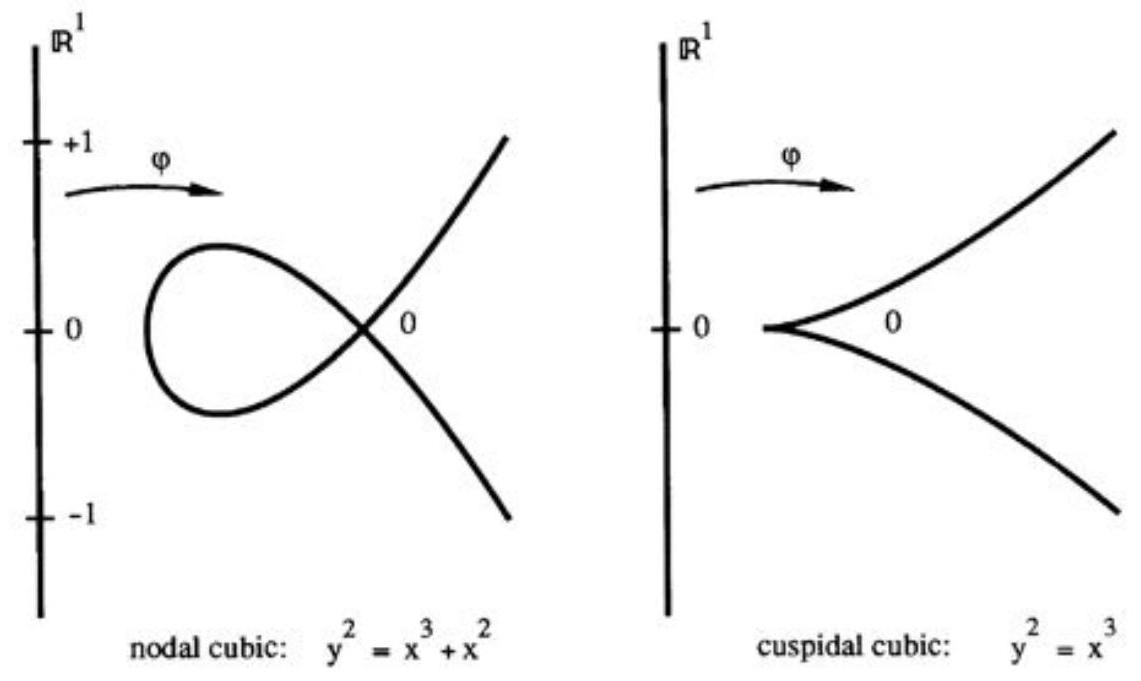
\includegraphics[max width=0.8\textwidth]{images/bo_d3lj80c601uc738kffi0_32_266_1160_1141_681_0.jpg}
\captionof{figure}{参数化三次曲线}
\end{center}
\hspace*{3em} 

请思考像、曲线以及映射 \(\varphi\) 的奇点.这些例子将在整个课程中反复出现，因此请花些时间研究这些方程；参见练习 2.1-2.

\section{曲线 \(y^2 = x(x-1)(x-\lambda)\) 没有有理参数化}

参数化曲线非常方便；例如，如果您对丢番图问题感兴趣，可能会期望有一个规则能给出所有的 \(\mathbb{Q}\)-值点，如 (1.1) 所示.(1.1) 的参数化形式为 \(x = f(t), y = g(t)\)，其中 \(f\) 和 \(g\) 是有理函数，即两个多项式的商.

\begin{theorem}
设 \(k\) 为特征不为 2 的域，且设 \(\lambda \in k\) 满足 \(\lambda \neq 0, 1\)；设 \(f, g \in k(t)\) 为满足以下条件的有理函数
\[
g^2 = f(f-1)(f-\lambda)
\]
则 \(f, g \in k\).
\end{theorem}

这等价于说，不存在任何由有理函数给出的非平凡映射 \(\mathbb{A}^1 \to C: y^2 = x(x-1)(x-\lambda)\).这反映了簇的一种非常强的“刚性”性质.

该定理的证明是在域 \(k(t)\) 上的算术，它利用了 \(k(t)\) 是唯一分解整环 (UFD) \(k[t]\) 的分式域这一事实.证明较长，您可以准备详细学习或暂时跳过（跳转至 2.4）.练习 2.12 中有一个通过在 \(\mathbb{Q}\) 上的算术进行不存在性证明的非常相似的例子.

\begin{proof}
利用 \(k[t]\) 是唯一分解整环的事实，我们写作
\[
f = p/q \quad \text{其中 } p, q \in k[t] \text{ 且互素，}
\]
\[
g = r/s \quad \text{其中 } r, s \in k[t] \text{ 且互素.}
\]
去分母后，原方程变为
\[
r^2 q^3 = s^2 p(p-q)(p-\lambda q)
\]
由于 \(r\) 和 \(s\) 互素，右侧的因子 \(s^2\) 必须整除 \(q^3\).同理，由于 \(p\) 和 \(q\) 互素，左侧的因子 \(q^3\) 必须整除 \(s^2\).因此，
\[
s^2 \mid q^3 \quad \text{且} \quad q^3 \mid s^2, \quad \text{从而 } s^2 = a q^3 \text{，其中 } a \in k^*
\]
（\(a\) 是 \(k[t]\) 的单位，因此属于 \(k\)）.
于是
\[
aq = (s/q)^2 \quad \text{是 } k[t] \text{ 中的一个平方.}
\]
此外，
\[
r^2 = a p(p-q)(p-\lambda q)
\]
因此通过考虑素因数分解，存在非零常数 \(b, c, d \in k\) 使得
\[
bp, \quad c(p-q), \quad d(p-\lambda q)
\]
都是 \(k[t]\) 中的平方.如果我能证明 \(p, q\) 是常数，那么根据前述内容，\(r, s\) 也将是常数，从而证明该定理.为了证明 \(p, q\) 是常数，设 \(K\) 为 \(k\) 的代数闭包；则 \(p, q \in K[t]\) 满足下一个引理的条件.
\end{proof}

\begin{lemma}
设 \(K\) 为代数闭域，\(p, q \in K[t]\) 为互素多项式.假设 4 个不同的线性组合（即对应于 4 个不同比值 \((\lambda : \mu) \in \mathbb{P}^1_K\) 的 \(\lambda p + \mu q\)）在 \(K[t]\) 中均为平方；则 \(p, q \in K\).
\end{lemma}

\begin{proof} (费马的“无限下降法”)
引理的假设和结论在用 \(p, q\) 替换为以下形式时不受影响
\[
p' = ap + bq, \quad q' = cp + dq,
\]
其中 \(a, b, c, d \in K\) 且 \(ad - bc \neq 0\).因此我们可以假设给定的 4 个平方是
\[
p, \quad p-q, \quad p-\lambda q, \quad q.
\]
则 \(p = u^2, q = v^2\)，且 \(u, v \in K[t]\) 互素.
现在通过反证法，假设 \(\max(\deg p, \deg q) > 0\) 且在所有满足引理条件的 \((p, q)\) 中取度数最小者.则
\[
p - q = u^2 - v^2 = (u-v)(u+v)
\]
和
\[
p - \lambda q = u^2 - \lambda v^2 = (u - \mu v)(u + \mu v)
\]
（其中 \(\mu = \sqrt{\lambda}\)）在 \(K[t]\) 中是平方.由 \(u, v\) 的互素性，我们得出 \(u-v, u+v, u-\mu v, u+\mu v\) 均为平方.这与 \(\max(\deg p, \deg q)\) 的最小性矛盾.
\end{proof}

\section{线性系统}\label{sec:linear-systems}

记 \(S_d = \{\text{次数为 } d \text{ 的齐次多项式}\} \subset k[X, Y, Z]\).任意元素 \(F \in S_d\) 可以唯一表示为
\[
F = \sum_{i+j+k=d} a_{ijk} X^i Y^j Z^k
\]
其中 \(a_{ijk} \in k\).这当然意味着 \(S_d\) 是一个以 \(k\) 为基的向量空间，其基为单项式：
\[
\begin{array}{cccc}
Z^d & & & \\
XZ^{d-1} & YZ^{d-1} & & \\
\vdots & & & \\
X^d & X^{d-1}Y & \dots & Y^d
\end{array}
\]
特别地，\(\dim S_d = \binom{d+2}{2}\).对于 \(P_1, \dots, P_n \in \mathbb{P}^2\)，定义
\[
S_d(P_1, \dots, P_n) = \{ F \in S_d \mid F(P_i) = 0 \text{ for } i=1, \dots, n \} \subset S_d.
\]
每个条件 \(F(P_i) = 0\)（更准确地说，是 \(F(X_i, Y_i, Z_i) = 0\)，其中 \(P_i = (X_i:Y_i:Z_i)\)）是对 \(F\) 的一个线性条件，因此 \(S_d(P_1, \dots, P_n)\) 是维数 \(\geq \binom{d+2}{2} - n\) 的向量空间.

\begin{lemma}
设 \(k\) 为无限域，且令 \(F \in S_d\).
\begin{enumerate}
    \item[(i)] 设 \(L \subset \mathbb{P}^2_k\) 为一条直线；若 \(F \equiv 0\) 在 \(L\) 上，则 \(F\) 在 \(k[X,Y,Z]\) 中可被 \(L\) 的方程整除.即，\(F = H \cdot F'\)，其中 \(H\) 是 \(L\) 的方程，且 \(F' \in S_{d-1}\).
    \item[(ii)] 设 \(C \subset \mathbb{P}^2_k\) 为非空非退化的圆锥曲线；若 \(F \equiv 0\) 在 \(C\) 上，则 \(F\) 在 \(k[X,Y,Z]\) 中可被 \(C\) 的方程整除.即，\(F = Q \cdot F'\)，其中 \(Q\) 是 \(C\) 的方程，且 \(F' \in S_{d-2}\).
\end{enumerate}
\end{lemma}

如果您认为这个命题显而易见，恭喜您的直觉：您刚刚猜到了零点定理 (Nullstellensatz) 的一个特例.现在请您自己寻找证明（或跳转至 2.6）.

\begin{proof}
(i) 通过坐标变换，我们可以假设 \(H = X\).那么对于任意 \(F \in S_d\)，存在唯一的表达式 \(F = X \cdot F'_{d-1} + G(Y, Z)\)：只需将所有含 \(X\) 的单项式归入第一个加数，剩下的必定是仅含 \(Y, Z\) 的多项式.现在
\[
F \equiv 0 \text{ on } L \iff G \equiv 0 \text{ on } L \iff G(Y, Z) = 0.
\]
最后一步成立是因为 (1.8)：若 \(G(Y, Z) \neq 0\)，则它在 \(\mathbb{P}^1_k\) 上最多有 \(d\) 个零点，而若 \(k\) 是无限的，则 \(\mathbb{P}^1_k\) 也是无限的.

(ii) 通过坐标变换，\(Q = XZ - Y^2\).现在我们来证明对于任意 \(F \in S_d\)，存在唯一的表达式
\[
F = Q \cdot F'_{d-2} + A(X, Z) + YB(X, Z)
\]
如果我们将 \(Y^2 = XZ - Q\) 代入 \(F\) 中所有出现的 \(Y^2\)，则关于 \(Y\) 的剩余项次数 \(\leq 1\)，因此其形式为 \(A(X, Z) + YB(X, Z)\).现在如同 (1.7)，\(C\) 是由 \(X=U^2, Y=UV, Z=V^2\) 给出的参数化圆锥曲线，因此
\[
F \equiv 0 \text{ on } C \iff A(U^2, V^2) + UVB(U^2, V^2) \equiv 0 \text{ on } C
\]
\[
\iff A(U^2, V^2) + UVB(U^2, V^2) = 0 \in k[U, V]
\]
\[
\iff A(X, Z) = 0 \text{ and } B(X, Z) = 0.
\]
这里最后的等价关系是通过分别考虑 \(A(U^2, V^2) + UVB(U^2, V^2)\) 中关于 \((U,V)\) 的偶次和奇次项得到的.
\end{proof}

练习 2.2 给出了类似的“显式”零点定理的例子.

\begin{corollary}
设 \(L: (H=0) \subset \mathbb{P}^2_k\) 为一条直线（或 \(C: (Q=0) \subset \mathbb{P}^2_k\) 为非退化圆锥曲线）；假设给定点 \(P_1, \dots, P_n \in \mathbb{P}^2_k\)，并考虑对某个固定的 \(d\)，\(S_d(P_1, \dots, P_n)\).则
\begin{enumerate}
    \item[(i)] 若 \(P_1, \dots, P_a \in L\)，\(P_{a+1}, \dots, P_n \notin L\) 且 \(a > d\)，则
    \[
    S_d(P_1, \dots, P_n) = H \cdot S_{d-1}(P_{a+1}, \dots, P_n).
    \]
    \item[(ii)] 如果 \(P_1, \dots, P_a \in C\)，\(P_{a+1}, \dots, P_n \notin C\) 且 \(a > 2d\)，则
    \[
    S_d(P_1, \dots, P_n) = Q \cdot S_{d-2}(P_{a+1}, \dots, P_n).
    \]
\end{enumerate}
\end{corollary}

\begin{proof}
(i) 如果 \(F\) 是 \(d\) 次齐次多项式，且曲线 \(D: (F=0)\) 在点 \(P_1, \dots, P_a\) 处与 \(L\) 相交，且满足 \(a > d\)，则根据 (1.9)，我们必须有 \(L \subset D\)，因此根据引理，\(F = H \cdot F'\)；现在由于 \(P_{a+1}, \dots, P_n \notin L\)，显然 \(F' \in S_{d-1}(P_{a+1}, \dots, P_n)\).(ii) 的证明完全相同.
\end{proof}

\begin{proposition}
设 \(k\) 是一个无限域，且有 \(P_1, \dots, P_8 \in \mathbb{P}^2_k\) 八个不同的点；假设 \(P_1, \dots, P_8\) 中没有 4 点共线，且没有 7 点位于同一条非退化二次曲线上，则
\[
\dim S_3(P_1, \dots, P_8) = 2.
\]
\end{proposition}

\begin{proof}
为简便起见，我们称一组点为“共二次曲线的”(conconic)，如果它们都位于同一条非退化二次曲线上.证明分为若干情况.

\textbf{主要情况：} 无 3 点共线，无 6 点共二次曲线.这是“一般位置”情况.

假设 \(\dim S_3(P_1, \dots, P_8) \geq 3\)，并令 \(P_9, P_{10}\) 是直线 \(L = P_1 P_2\) 上的不同点.则
\[
\dim S_3(P_1, \dots, P_{10}) \geq \dim S_3(P_1, \dots, P_8) - 2 \geq 1,
\]
因此存在 \(0 \neq F \in S_3(P_1, \dots, P_{10})\).根据推论 2.5，\(F = H \cdot Q\)，且满足 \(Q \in S_2(P_3, \dots, P_8)\).现在我们得到了与情况假设的矛盾：如果 \(Q\) 是非退化的，则 6 点 \(P_3, \dots, P_8\) 共二次曲线；而如果 \(Q\) 是一对直线或重直线，则至少 3 点共线.

\begin{center}
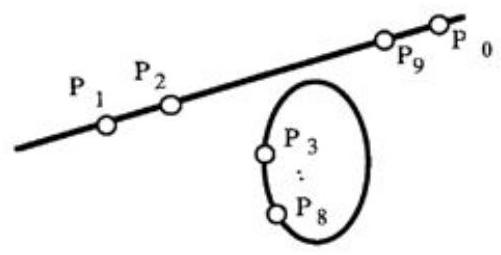
\includegraphics[max width=0.3\textwidth]{images/bo_d3lj80c601uc738kffi0_36_587_1142_501_255_0.jpg}
\captionof{figure}{一个可约三次曲线上的10个点}
\end{center}
\hspace*{3em} 

\textbf{第一退化情况：} 假设 \(P_1, P_2, P_3 \in L\) 共线，且令 \(L: (H=0)\).令 \(P_9\) 是直线 \(L\) 上的第 4 个点.则根据推论 2.5，
\[
S_3(P_1, \dots, P_9) = H \cdot S_2(P_4, \dots, P_8).
\]
此外，由于 \(P_4, \dots, P_8\) 中没有 4 点共线，根据推论 1.11，
\[
\dim S_2(P_4, \dots, P_8) = 1, \quad \text{那么} \quad \dim S_3(P_1, \dots, P_9) = 1,
\]
这意味着 \(\dim S_3(P_1, \dots, P_8) \leq 2\).

\textbf{第二退化情况：} 假设 \(P_1, \dots, P_6 \in C\) 共二次曲线，且 \(C: (Q=0)\) 是非退化二次曲线.然后选择与 \(P_1, \dots, P_6\) 不同的 \(P_9 \in Q\).再次根据推论 2.5，
\[
S_3(P_1, \dots, P_9) = Q \cdot S_1(P_7, P_8);
\]
直线 \(L = P_7 P_8\) 是唯一的，因此 \(S_3(P_1, \dots, P_9)\) 是由 \(QL\) 张成的一维空间，从而 \(\dim S_3(P_1, \dots, P_8) \leq 2\).
\end{proof}

\begin{corollary}[Cayley-Bacharach 定理]
设 \(C_1, C_2\) 为两条三次曲线，其交点由 9 个不同点组成，\(C_1 \cap C_2 = \{P_1, \dots, P_9\}\).则任何经过 \(P_1, \dots, P_8\) 的三次曲线 \(D\) 也必定经过 \(P_9\).
\end{corollary}

\begin{proof}
若 4 个点（例如 \(P_1, \dots, P_4\)）位于一条直线 \(L\) 上，则 \(C_1\) 和 \(C_2\) 各自与 \(L\) 相交于 \(\geq 4\) 个点，因此都包含 \(L\)，这与对 \(C_1 \cap C_2\) 的假设矛盾.出于完全相同的理由，不能有 7 个点共二次曲线.因此满足 (2.6) 的假设，故我们可以得出结论
\[
\dim S_3(P_1, \dots, P_8) = 2.
\]
这意味着两条三次曲线 \(C_1, C_2\) 的方程 \(F_1, F_2\) 构成 \(S_3(P_1, \dots, P_8)\) 的一组基.因此 \(D\) 的方程 \(G\) 可以写为 \(G = \lambda F_1 + \mu F_2\).现在 \(F_1, F_2\) 在 \(P_9\) 处为零，因此 \(G\) 在 \(P_9\) 处也为零.
\end{proof}

\section{平面三次曲线上的群运算}

设 \(k \subset \mathbb{C}\) 是 \(\mathbb{C}\) 的一个子域，\(F \in k[X,Y,Z]\) 是定义（非空）平面曲线 \(C: (F=0) \subset \mathbb{P}^2_k\) 的三次齐次多项式.假设 \(F\) 满足以下两个条件：
\begin{enumerate}
    \item[(a)] \(F\) 是不可约的（因此 \(C\) 不包含直线或二次曲线作为分量）；
    \item[(b)] 对每个点 \(P \in C\)，存在唯一一条直线 \(L \subset \mathbb{P}^2_k\)，使得 \(P\) 是 \(F|_L\) 的重根.
\end{enumerate}
注意，从几何角度看，条件 (b) 表示 \(C\) 应为非奇异的，所指的直线 \(L\) 是切线 \(L = T_P C\)（参见练习 2.3）.这将在第 6 章中成为非奇异性和簇的切空间一般定义的动机.

固定任意一点 \(O \in C\)，进行如下构造：

\textbf{构造}
\begin{enumerate}
    \item[(i)] 对 \(A \in C\)，令 \(\bar{A}\) 为 \(C\) 与直线 \(OA\) 的第三个交点；
    \item[(ii)] 对 \(A, B \in C\)，记 \(R\) 为 \(AB\) 与 \(C\) 的第三个交点，并通过 \(A+B = \bar{R}\) 定义和.
\end{enumerate}

\begin{center}
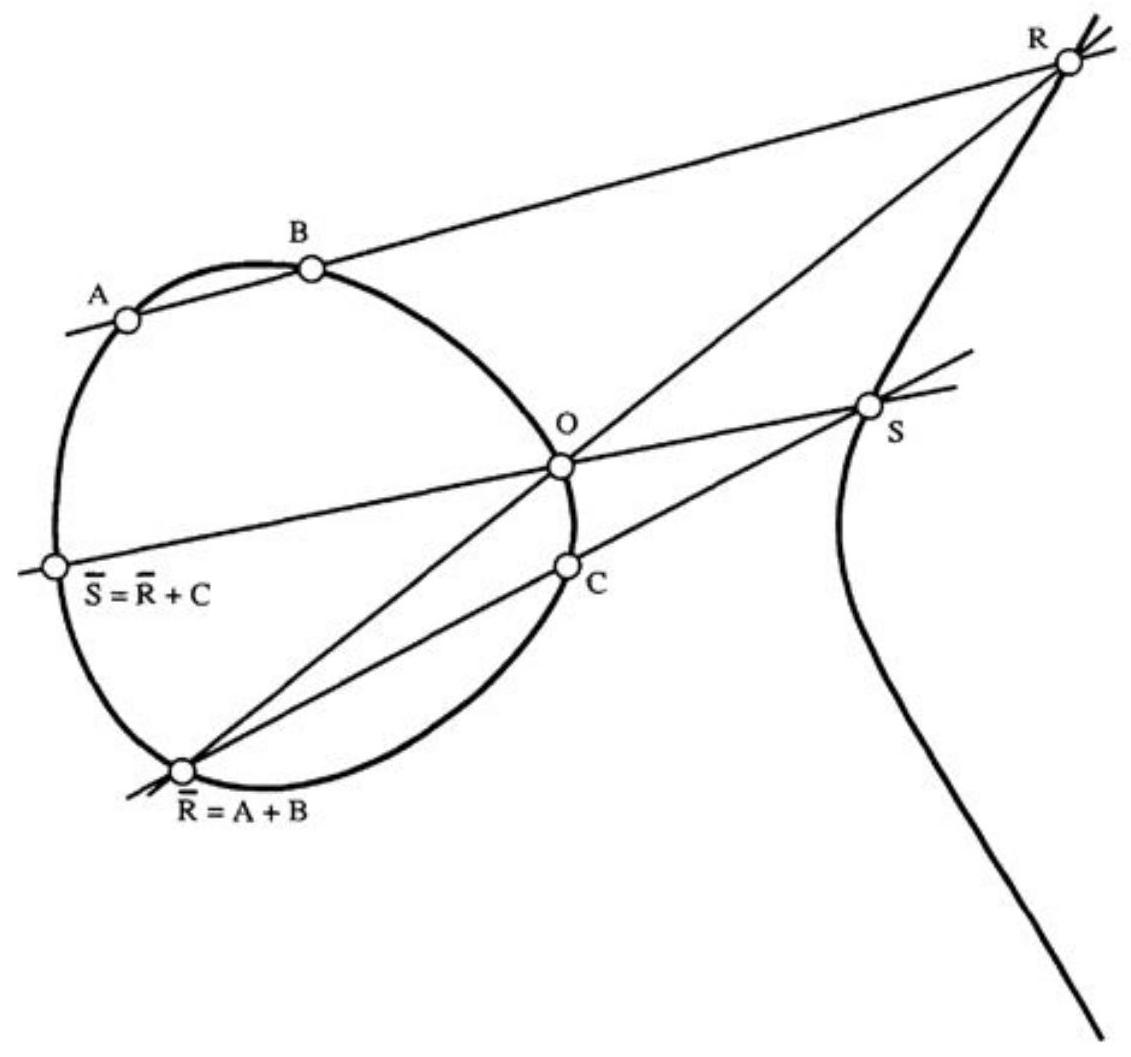
\includegraphics[max width=0.8\textwidth]{images/bo_d3lj80c601uc738kffi0_38_276_641_1131_1057_0.jpg}
\captionof{figure}{三次曲线及其群运算}
\end{center}
\hspace*{3em} 

\begin{theorem}
上述构造在 \(C\) 上定义了一个阿贝尔群运算，以 \(O\) 作为零元（单位元）.
\end{theorem}

\begin{proof}
结合律是关键；我们先从简单部分开始证明.

(I) \textbf{良定义性}：我们必须证明加法和逆元运算是良定义的.如果 \(P, Q \in C\) 是任意两点，那么要么 \(P \neq Q\)，此时直线 \(L = PQ \subset \mathbb{P}^2_k\) 是唯一确定的；要么 \(P = Q\)，此时根据假设 (b)，存在唯一一条直线 \(L \subset \mathbb{P}^2_k\) 使得 \(P\) 是 \(F|_L\) 的重根.无论哪种情况，\(F|_L\) 都是关于两个变量的三次齐次多项式，它有两个给定的 \(k\)-值零点.因此它可以分解为三个线性因子的乘积，故第三个剩余交点 \(R\) 是定义良好的，且其坐标属于 \(k\).注意，允许任意的 \(P=Q, P=R, Q=R\) 或 \(P=Q=R\)；这些在代数上对应于 \(F|_L\) 具有重根，在几何上对应于切点和拐点.

(II) \textbf{单位元}：验证给定点 \(O\) 是单位元完全是形式上的.由于 \(O, A, \bar{A}\) 共线，构造 \(O+A\) 包括取直线 \(L=OA\) 得到第三个交点 \(\bar{A}\)，然后用同一条直线 \(L=O\bar{A}\) 返回到 \(A\).

(III) \textbf{交换律}：\(A+B = B+A\) 留给读者作为练习.

(IV) \textbf{逆元}：首先定义构造中 (i) 所述的点 \(\bar{O}\)：设 \(L_0\) 为一条直线，使得 \(F|_{L_0}\) 在 \(O\) 处有重根，并定义 \(\bar{O}\) 为 \(L_0\) 与 \(C\) 的第三个交点.然后容易验证，对于每个 \(A \in C\)，\(A\) 的逆元是 \(\bar{O}A\) 与 \(C\) 的第三个交点.
\end{proof}

\section{一般情况下的结合律}

现在我们给出“足够一般”点的结合律证明.假设 \(A, B, C\) 是 \(C\) 上的三个给定点.则 \((A+B)+C = \bar{S}\) 的构造使用了 4 条直线（见上图）：
\[
L_1: ABR, \quad L_2: RO\bar{R}, \quad L_3: C\bar{R}S, \quad L_4: SO\bar{S}.
\]
而 \((B+C)+A = \bar{T}\) 的构造使用了 4 条直线：
\[
M_1: BCQ, \quad M_2: QO\bar{Q}, \quad M_3: A\bar{Q}T, \quad M_4: TO\bar{T}.
\]
我们想证明 \(\bar{S} = \bar{T}\)，为此只需证明 \(S=T\).考虑两个（可约的）三次曲线
\[
D_1 = L_1 \cup M_2 \cup L_3 \quad \text{和} \quad D_2 = M_1 \cup L_2 \cup M_3.
\]
根据构造，
\[
C \cap D_1 = \{A, B, C, O, R, \bar{R}, Q, \bar{Q}, S\},
\]
\[
C \cap D_2 = \{A, B, C, O, R, \bar{R}, Q, \bar{Q}, T\}.
\]
只要这 9 个点 \(A, B, C, O, R, \bar{R}, Q, \bar{Q}, S\) 均不相同，两条三次曲线 \(C\) 和 \(D_1\) 就满足推论 2.7 的条件.因此，\(D_2\) 必定经过 \(S\).如果 \(S\) 不在 \(D_2\) 的任何分量上，这唯一可能的情况是 \(S=T\).

要完成这个论证有多种方法.其中最彻底的方法是真正处理两条曲线的交点，考虑多重交点（大致用“交点理想”表示），与推论 2.7 对应的陈述是 Max Noether 引理（参见 [Fulton, pp. 120, 124]）.

\section{连续性证明}

我们简述一种“连续性”论证方法，它利用了 \(k \subset \mathbb{C}\) 的事实.记 \(C_\mathbb{C} \subset \mathbb{P}^2_\mathbb{C}\) 为复化曲线 \(C\)，即满足同一方程 \(F(X,Y,Z)=0\) 的复数比值集合 \((X:Y:Z)\).若结合律对所有 \(A, B, C \in C_\mathbb{C}\) 成立，则显然对 \(C\) 中的所有点也成立.因此，我们可以假设 \(k = \mathbb{C}\).

关心此事的读者不难找到以下两条陈述的证明（见练习 2.8）：

\begin{lemma}
\begin{enumerate}
    \item[(i)] \(A+B\) 是 \(A\) 和 \(B\) 的连续函数.
    \item[(ii)] 对于所有 \(A, B, C \in C\)，存在任意接近 \(A, B, C\) 的 \(A', B', C' \in C\)，使得由它们构造的 9 个点 \(A', B', C', O, R, \bar{R}, Q, \bar{Q}, S\) 均不相同.
\end{enumerate}
\end{lemma}

加法法则是映射 \(\varphi: C \times C \to C\)，由 \((A, B) \mapsto A+B\) 给出.根据 (i)，\(\varphi\) 是连续的，因此以下两个复合映射也是连续的：
\[
f = \varphi \circ (\varphi \times \operatorname{id}_C) \quad \text{和} \quad g = \varphi \circ (\operatorname{id}_C \times \varphi) : C \times C \times C \to C
\]
它们分别由 \((A, B, C) \mapsto (A+B)+C\) 和 \(A+(B+C)\) 给出.此外，根据 (ii)，使得构造中 9 个点均不同的三元组 \((A, B, C)\) 组成的子集 \(U \subset C \times C \times C\) 是稠密的.由上述论证，\(f\) 和 \(g\) 在 \(U\) 上重合，且因其连续性，故在任何地方都重合.

\textbf{备注}：连续性论证如其所述涉及 \(\mathbb{C}\) 的拓扑，因此并非纯代数的.事实上，加法映射 \(\varphi\) 是簇 (varieties) 的态射 \(\varphi: C \times C \to C\)，我们稍后将证明这一点（见 (4.14)）.其余论证也可以用这种纯代数形式重新表述：使得 9 个点互异的 \(C \times C \times C\) 的子集是 Zariski 拓扑下的稠密开集，而两个在稠密开集上重合的态射必定在全体上重合.（希望此备注能为课程其余部分提供有用的动机；若感到困惑，暂时可忽略.）

\section{帕斯卡定理 (神秘六边形)}

图中包含一个内接于二次曲线的六边形 \(ABCDEF \subset \mathbb{P}^2_k\)，其对边成对延长直至在点 \(P, Q, R\) 相交.假设图中的九点和六条直线均互不相同.

\begin{center}
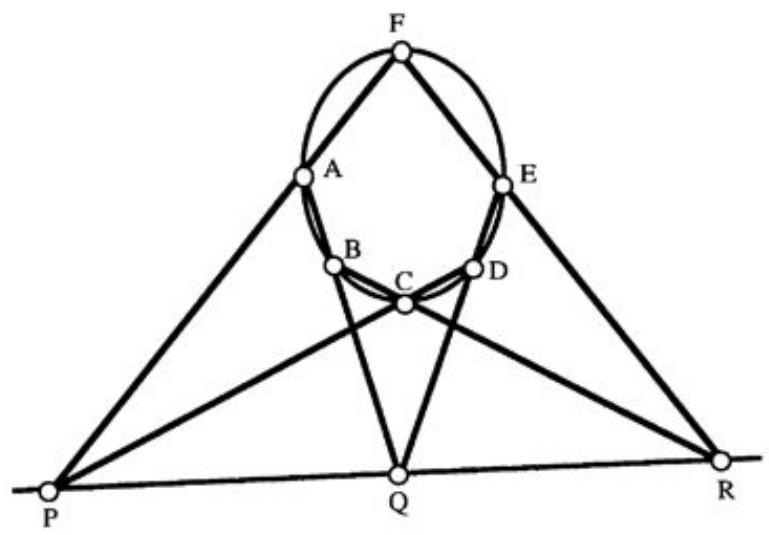
\includegraphics[max width=0.6\textwidth]{images/bo_d3lj80c601uc738kffi0_40_464_1080_769_535_0.jpg}
\captionof{figure}{神秘六边形}
\end{center}
\hspace*{3em} 

\begin{theorem}[帕斯卡定理]
六点 \(A, B, C, D, E, F\) 共二次曲线 \(\iff\) 三点 \(P, Q, R\) 共线.
\end{theorem}

这个著名定理是 (2.7) 的一个相当类似的应用，此处仅为趣味而给出.当然，也有其他证明方法，参见任何几何教材，例如 [Berger, 16.2.10 和 16.8.3-5].

\begin{proof}
在图中，考虑两组三条直线
\[
L_1: PAF, \quad L_2: QDE, \quad L_3: RBC,
\]
和
\[
M_1: PCD, \quad M_2: QAB, \quad M_3: REF.
\]
设 \(C_1 = L_1 \cup L_2 \cup L_3\) 和 \(C_2 = M_1 \cup M_2 \cup M_3\).显然 \(C_1\) 和 \(C_2\) 是两条三次曲线，且满足
\[
C_1 \cap C_2 = \{A, B, C, D, E, F, P, Q, R\}.
\]
\(\implies\): 假设 \(P, Q, R\) 共线，设 \(L\) 为过这三点的直线.设 \(\Gamma\) 为经过 \(A, B, C, D, E\) 的二次曲线（其存在性和唯一性由命题 1.11 保证）.则 \(L \cup \Gamma\) 是一个经过 8 个点 \(A, B, C, D, E, P, Q, R\) 的三次曲线.依据 (2.7)，它必包含第 9 个点 \(F\).根据假设，\(F \notin L\)，因此必然有 \(F \in \Gamma\)，证明这六点共二次曲线.

\(\impliedby\): 反之，假设 \(A, B, C, D, E, F\) 位于二次曲线 \(\Gamma\) 上.设 \(L = PQ\).则 \(L \cup \Gamma\) 是经过 \(A, B, C, D, E, F, P, Q\) 这 8 个点的三次曲线，故根据 (2.7) 它必经过第 9 个点 \(R\).现在 \(R\) 不可能位于二次曲线 \(\Gamma\) 上（否则 \(\Gamma\) 是两条直线的组合，且图中的六条直线中必有重合），因此 \(R \in L\)，即 \(P, Q, R\) 共线.
\end{proof}

\section{拐点与标准形}

\(\mathbb{P}^2_\mathbb{R}\) 或 \(\mathbb{P}^2_\mathbb{C}\) 中的任意非奇异三次曲线均可经过射影变换化为标准形（魏尔斯特拉斯范式）
\[
Y^2 Z = X^3 + aXZ^2 + bZ^3,
\]
或其仿射形式
\[
y^2 = x^3 + ax + b.
\]
现在考虑上述曲线 \(C\).它与无穷远直线 \(L: (Z=0)\) 相交于何处？只需将 \(Z=0\) 代入定义多项式 \(F = -Y^2 Z + X^3 + aXZ^2 + bZ^3\)，得到 \(F|_L = X^3\).这意味着 \(F|_L\) 在点 \(O = (0:1:0)\) 处有三重根.为理解其几何意义，设 \(Y=1\)，得到以 \((0:1:0)\) 为中心的仿射坐标 \((x, z)\) 下的方程：
\[
z = x^3 + axz^2 + bz^3.
\]
该曲线在原点附近可被 \(z = x^3\) 高度精确地近似.

\begin{center}
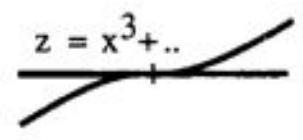
\includegraphics[max width=0.2\textwidth]{images/bo_d3lj80c601uc738kffi0_41_793_1592_303_140_0.jpg}
\captionof{figure}{拐点}
\end{center}
\hspace*{3em} 

这表示 \(C\) 在 \((0:1:0)\) 处有一个拐点.更一般地，曲线 \(C\) 上的拐点 \(P\) 定义为存在一条直线 \(L \subset \mathbb{P}^2_k\)，使得 \(F|_L\) 在 \(P\) 处有重数 \(\geq 3\) 的根（参见练习 2.9；实际上根据 (2.8, b) 必然有 \(L = T_P C\)，重数由 (1.9) 确定）.用定义方程的导数和二阶导数来解释这一点并不难：例如，如果定义方程是 \(y = f(x)\)，那么拐点的条件就是 \(\frac{d^2 f}{dx^2}(P) = 0\).这在图中对应曲线从“下凹”到“上凹”的转变.关于平面曲线存在拐点的一般判据可用 Hessian 矩阵表示，详见 [Fulton, p. 116] 或练习 7.3 (iii).

可以证明（参见练习 2.10），反之若平面三次曲线 \(C\) 有一个拐点，则其方程可化为上述的标准形式.

\section{简化的群运算律}

标准形式对于群运算律极为方便：取拐点 \(O = (0:1:0)\) 作为单位元.在此条件下，群运算律特别简洁，原因如下：
\begin{enumerate}
    \item[(a)] \(C = \{O\} \cup C_0\)，其中 \(C_0\) 是仿射曲线 \(y^2 = x^3 + ax + b\).因此将 \(C\) 视为仿射曲线是合理的，偶尔提及无穷远点 \(O\)，即群运算的零元.
    \item[(b)] 通过 \(O\) 的直线是构造群运算 (2.8, i) 的主要元素.这些直线在射影意义下由 \(X = \lambda Z\) 给出，在仿射意义下由 \(x = \lambda\) 给出.任意此类直线与 \(C\) 相交于点 \((\lambda, \pm \sqrt{\lambda^3 + a\lambda + b})\) 及无穷远点 \(O\).因此若 \(P = (x, y)\)，则 (2.8, i) 中构造的点 \(\bar{P}\) 为 \((x, -y)\).故 \(P \mapsto \bar{P}\) 是曲线 \(C_0\) 关于 \(x\)-轴的自然对称 \((x, y) \mapsto (x, -y)\).
\end{enumerate}

\begin{center}
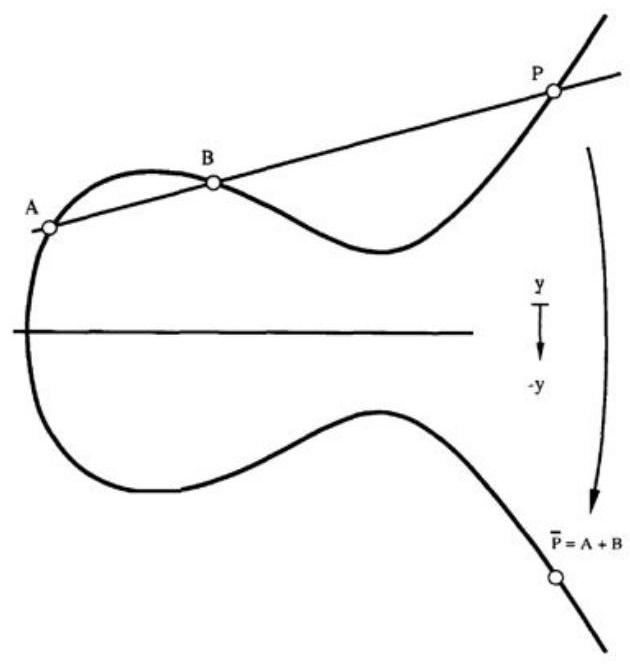
\includegraphics[max width=0.4\textwidth]{images/bo_d3lj80c601uc738kffi0_42_528_1157_630_664_0.jpg}
\captionof{figure}{以 \(x\) 轴为反射轴的取负运算}
\end{center}
\hspace*{3em} 

\begin{enumerate}
    \item[(c)] 群运算 (2.8, IV) 的逆元通过 \(\bar{O}\) 描述，该点是 \(C\) 与其在 \(O\) 处的切线的第三个交点.在本例中，该切线是无穷远直线 \(L: (Z=0)\)，且 \(L \cap C = 3O\)，因此 \(\bar{O} = O\).群运算的逆元简化为 \(-P = \bar{P}\).
\end{enumerate}

我们现在可以将群运算律重新表述为定理 2.8 的一个大大简化的版本：

\begin{theorem}
设 \(C\) 是标准形式的三次曲线；则在 \(C\) 上存在唯一的群运算，使得 \(O = (0:1:0)\) 是单位元，逆元由 \((x, y) \mapsto (x, -y)\) 给出，且对所有 \(P, Q, R \in C\)，
\[
P + Q + R = O \iff P, Q, R \text{ 共线.}
\]
\end{theorem}

\section{第二章习题}

\begin{exercise}
设 \(C: y^2 = x^3 + x^2 \subset \mathbb{R}^2\).证明通过原点 \((0,0)\) 的一条变量直线与 \(C\) 还有一个交点，由此推导出 (2.1) 中给出的 \(C\) 的参数化.对 \(y^2 = x^3\) 和 \(x^3 = y^3 - y^4\) 也做同样的操作.
\end{exercise}

\begin{exercise}
设 \(\varphi: \mathbb{R}^1 \to \mathbb{R}^2\) 是由 \(t \mapsto (t^2, t^3)\) 给出的映射.直接证明任何在像 \(C = \varphi(\mathbb{R}^1)\) 上为零的多项式 \(f \in \mathbb{R}[X, Y]\) 都能被 \(Y^2 - X^3\) 整除.[提示：使用引理 2.5 中的方法.] 确定域 \(k\) 需具备何种性质才能保证对由相同公式给出的 \(\varphi: k \to k^2\) 结果成立.
对 \(t \mapsto (t^2 - 1, t^3 - t)\) 也做同样的操作.
\end{exercise}

\begin{exercise}
设 \(C: (f=0) \subset k^2\)，且设 \(P=(a,b) \in C\).假设 \(\frac{\partial f}{\partial x}(P) \neq 0\) 或 \(\frac{\partial f}{\partial y}(P) \neq 0\).证明直线
\[
L: \frac{\partial f}{\partial x}(P) \cdot (x-a) + \frac{\partial f}{\partial y}(P) \cdot (y-b) = 0
\]
是 \(C\) 在 \(P\) 处的切线，即 \(k^2\) 中唯一一条使得 \(f|_L\) 在 \(P\) 处有重根的直线（详见 (6.1) 中的推导）.
\end{exercise}

\begin{exercise}
设 \(C: y^2 = x^3 + 4x\)，采用简化的群运算 (2.13).证明 \(C\) 在 \(P=(2,4)\) 处的切线经过原点 \((0,0)\)，由此推断 \(P\) 是该群运算中的一个 4 阶点.
\end{exercise}

\begin{exercise}
设 \(C: y^2 = x^3 + ax + b \subset \mathbb{R}^2\) 是非奇异的.找出群运算中所有的 2 阶点，并理解它们构成的群（需考虑两种情况）.然后几何上说明如何寻找 \(C\) 上所有的 4 阶点.
\end{exercise}

\begin{exercise}
设 \(C: y^2 = x^3 + ax + b \subset \mathbb{R}^2\).编写一个计算机程序绘制 \(C\) 的部分图形，并计算群运算.程序应提示输入两点 \(A\) 和 \(B\) 的坐标，随后绘制直线并输出 \(A+B\) 的坐标.（使用实数变量.）
\end{exercise}

\begin{exercise}
设 \(C: y^2 = x^3 + ax + b \subset k^2\).若 \(A=(x_1, y_1)\) 且 \(B=(x_2, y_2)\)，说明如何将 \(A+B\) 的坐标表示为 \(x_1, y_1, x_2, y_2\) 的有理函数.[提示：若 \(F(X)\) 是三次多项式且已知两个根，则可通过观察 \(F\) 的一个系数找到第三个根.此题答案不唯一，因为有多种正确的有理函数表达式.一个解见 (4.14).]
\end{exercise}

\begin{exercise}
通过写出 \(C\) 在 \(A\) 处切线的方程，求出群运算中 \(C\) 上 \(2A\) 的公式，并验证当 \(B\) 趋近于 \(A\) 时，该公式是 \(A+B\) 公式的极限.[提示：使用练习 2.7，必要时参考 (4.14).]
\end{exercise}

\begin{exercise}
设 \(x, z\) 为 \(k^2\) 上的坐标，且设 \(f \in k[x, z]\).将 \(f\) 写成
\[
f = a + bx + cz + dx^2 + exz + fz^2 + \dots
\]
用系数 \(a, b, c, \dots\) 表示必须满足的条件，以保证
\begin{enumerate}
    \item[(i)] \(P=(0,0) \in C: (f=0)\);
    \item[(ii)] \(C\) 在 \(P\) 处的切线是 \(z=0\);
    \item[(iii)] \(P\) 是 \(C\) 的一个拐点，且切线为 \(z=0\).
\end{enumerate}
(回顾 (2.12)，若切线 \(L\) 存在，且 \(f|_L\) 在 \(P\) 处至少有三重根，则 \(P \in C\) 为拐点.)
\end{exercise}

\begin{exercise}
设 \(C \subset \mathbb{P}^2_k\) 为平面三次曲线，假设 \(P \in C\) 是一个拐点.证明通过在 \(\mathbb{P}^2_k\) 中变换坐标，可以将 \(C\) 化为标准形式
\[
Y^2 Z = X^3 + aX^2 Z + bXZ^2 + cZ^3.
\]
[提示：取坐标使得 \(P=(0:1:0)\) 及拐点切线为 \(Z=0\).利用前一题，在局部坐标 \((x,z)\) 中，\(Y\) 将以二次项 \(Y^2 Z\) 出现，其余仅线性出现.然后通过配方法消去 \(Y\) 中的线性项.]
\end{exercise}

\begin{exercise}[尖点三次曲线上的群运算]
考虑曲线 \(C: z = x^3 \subset k^2\).\(C\) 是双射映射 \(\varphi: k \to C\)（由 \(t \mapsto (t, t^3)\) 给出）的像，因此继承了加法群 \(k\) 的群结构.证明这是 \(C\) 上唯一的群运算，使得 \((0,0)\) 为单位元且
\[
P+Q+R=0 \iff P, Q, R \text{ 共线}
\]
对于 \(P, Q, R \in C\).[提示：你可能会发现恒等式
\[
\det \begin{vmatrix} 1 & a & a^3 \\ 1 & b & b^3 \\ 1 & c & c^3 \end{vmatrix} = (a-b)(b-c)(c-a)(a+b+c).
\]
在射影几何的术语中，\(C\) 是曲线 \(Y^2 Z = X^3\)，即我们熟悉的在原点有尖点且在 \((0:1:0)\) 有拐点的曲线.本题的关键是，通常的构造在奇点的补集上给出了群运算.]
\end{exercise}

\begin{exercise}[由莱昂纳多·斐波那契于公元1220年提出]
证明对于 \(u, v \in \mathbb{Z}\)，
\[
u^2+v^2 \text{ 和 } u^2-v^2 \text{ 均为平方数 } \implies v=0.
\]
提示 (由皮埃尔·德·费马提供，见 J.W.S. Cassels, J. London Math. Soc. 41 (1966), p. 207):
\begin{enumerate}
    \item[第一步] 化简为求解 \(x^2 = u^2+v^2, y^2 = u^2-v^2\)，其中 \(x, y, u, v \in \mathbb{Z}\) 两两互质.
    \item[第二步] 模 4 的考虑表明 \(x, y, u\) 是奇数，\(v\) 是偶数.
    \item[第三步] 因式分解方程 \((x-u)(x+u)=v^2\) 和 \((u-y)(u+y)=v^2\).
    \item[第四步] 证明 \(x-u=2v_1^2, u-y=2u_1^2, x-y=2x_1^2\) 和 \(2u-x-y=2y_1^2\)，其中 \(u_1, v_1, x_1, y_1 \in \mathbb{Z}\).
    \item[第五步] 证明 \(u_1, v_1, x_1, y_1\) 是原方程的另一个解，且满足 \(v_1 < v\)，并通过“无限下降法”推导出矛盾.
\end{enumerate}
请将此论证与 (2.2) 的证明进行比较，后者更简单，仅因为我们不必处理 2 的幂次问题.
\end{exercise}

\chapter*{附录：曲线及其亏格}

\section{非奇异三次曲线的拓扑}

我们不难看出，一条非奇异的实平面三次曲线 \(C: y^2 = x^3 + ax + b \subset \mathbb{P}^2_\mathbb{R}\) 具有以下两种形态之一：

\begin{figure}[ht]
\centering
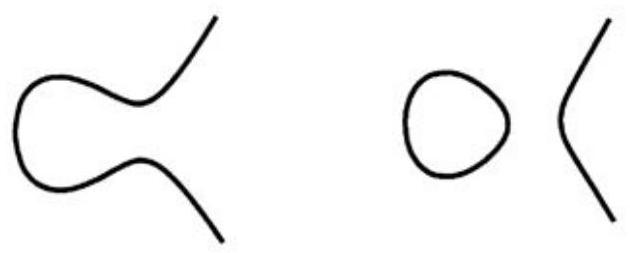
\includegraphics[max width=0.4\textwidth]{images/bo_d3lj80c601uc738kffi0_46_521_964_630_253_0.jpg}
\caption{实三次曲线的两种形态}
\end{figure}

从拓扑角度看，\(C\) 的实部要么是一个圆，要么是两个圆（包含无穷远点）。

为了在复数域 \(\mathbb{C}\) 上考察同样的问题，我们采用另一种标准形式：
\[
C: y^2 = x(x-1)(x-\lambda) \cup \{\infty\}
\]
那么，\(C \subset \mathbb{P}^2_\mathbb{C}\) 的拓扑结构是什么？答案是：一个环面。

\begin{figure}[ht]
\centering
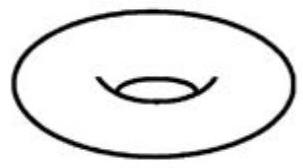
\includegraphics[max width=0.2\textwidth]{images/bo_d3lj80c601uc738kffi0_46_689_1557_303_168_0.jpg}
\caption{环面}
\end{figure}

证明的思路是考虑映射
\[
\pi: C \to \mathbb{P}^1_\mathbb{C} \quad \text{by} \quad (X:Y:Z) \mapsto (X:Z) \quad \text{and} \quad \infty \mapsto (1:0);
\]
在仿射坐标中，这是 \((x,y) \mapsto x\)。因此，这是一个 2-1 映射，对应于 \(y = \pm \sqrt{x(x-1)(x-\lambda)}\) 的图像。我们知道，\(\mathbb{P}^1_\mathbb{C}\) 与黎曼球面同胚（通过球极投影）。现在，我们来考虑定义在 \(\mathbb{P}^1_\mathbb{C}\) 上的“函数” \(y(x) = \pm \sqrt{x(x-1)(x-\lambda)}\)。在分支点 \(\{0, 1, \lambda, \infty\}\) 之外，这是一个二值函数。

\begin{figure}[ht]
\centering
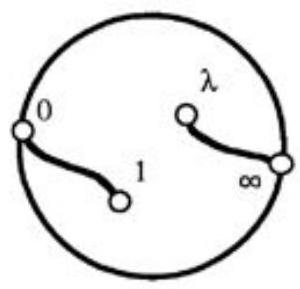
\includegraphics[max width=0.2\textwidth]{images/bo_d3lj80c601uc738kffi0_47_801_471_300_289_0.jpg}
\caption{连接分支点的两条路径：[0,1] 和 [\(\lambda, \infty\)]}
\end{figure}

现在，我们沿着连接分支点的两条路径 [0,1] 和 \([\lambda, \infty]\) 切开黎曼球面 \(\mathbb{P}^1_\mathbb{C}\)。这个二重覆盖分解为两个部分，函数 \(y\) 在每个分支上都是单值的。（阴影表示两张分支的匹配方式）

\begin{figure}[ht]
\centering
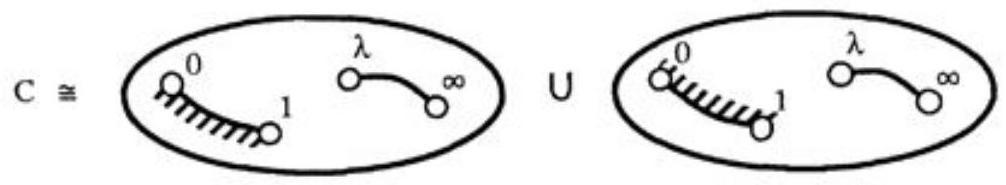
\includegraphics[max width=0.7\textwidth]{images/bo_d3lj80c601uc738kffi0_47_445_997_1006_185_0.jpg}
\caption{\(C\) 作为两个带裂缝球面的并集}
\end{figure}

为了理解其拓扑结构，我们将裂缝打开：

\begin{figure}[ht]
\centering
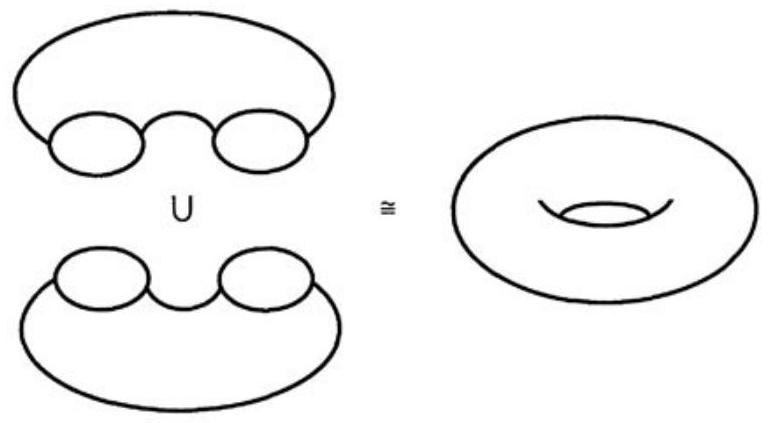
\includegraphics[max width=0.6\textwidth]{images/bo_d3lj80c601uc738kffi0_47_566_1379_768_423_0.jpg}
\caption{将两个带裂缝的球面粘合得到环面}
\end{figure}

\section{关于曲面亏格的讨论}

定义在 \(\mathbb{C}\) 上的非奇异射影曲线 \(C\) 只有一个拓扑不变量，即其亏格 \(g = g(C)\)：

\begin{figure}[ht]
\centering
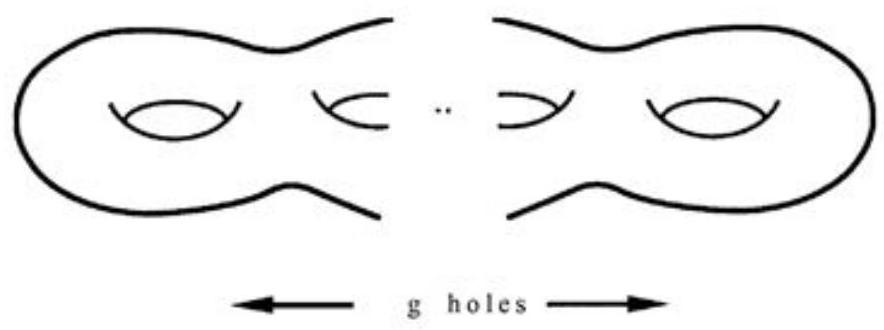
\includegraphics[max width=0.6\textwidth]{images/bo_d3lj80c601uc738kffi0_48_396_449_884_330_0.jpg}
\caption{亏格为 \(g\) 的曲面}
\end{figure}

例如，仿射曲线 \(C: y^2 = f_{2g+1}(x) = \prod_i (x-a_i) \subset \mathbb{C}^2\)，其中 \(f_{2g+1}\) 是一个具有 \(2g+1\) 个不同根 \(a_i\) 的多项式。我们可以像 (2.13) 中那样，将其与 \(\sqrt{f}\) 的黎曼曲面联系起来，并视其为在 \(2g+1\) 个点 \(a_i\) 及无穷远点 \(\infty\) 处分歧的黎曼球面 \(\mathbb{P}^1_\mathbb{C}\) 的二重覆盖。通过相同的论证，可以看出其亏格为 \(g\)。

另一个重要的例子是，一条次数为 \(d\) 的非奇异平面曲线 \(C_d \subset \mathbb{P}^2_\mathbb{C}\) 的亏格由其次数决定，公式为 \(g(C_d) = \binom{d-1}{2}\)。

\section{延伸阅读}

复曲线（即紧致黎曼曲面）出现在数学的各个领域，从丢番图算术、复分析、低维拓扑到数学物理中的微分方程。因此，深入学习复曲线是很有价值的。

曲线的性质在很大程度上由其亏格决定，特别是根据三分法 \(g=0, g=1\) 或 \(g \geq 2\) 来划分。下页的表格描述了其中一些更显著的方面，我们也将进行简要讨论。这些内容应当成为每位数学家的背景知识。

为了部分回答 (1.1-2) 和 (2.1) 中提到的丢番图问题，我们已知一条曲线当且仅当其亏格 \(g=0\) 时，才可以用有理函数参数化。如果我们在一个固定域 \(k\) 上工作，亏格为 0 的曲线可能没有任何 \(k\)-值点（例如 (1.2) 中的圆锥曲线），但如果它有一个 \(k\)-值点，那么它就可以在 \(k\) 上被参数化，使得其 \(k\)-值点与 \(\mathbb{P}^1_k\) 一一对应。

任何亏格为 1 的曲线都同构于本节中的三次曲线，并且在其 \(k\)-值点集上可以定义一个群运算（当然前提是至少存在一个点——不存在空群）。如果 \(k\) 是一个数域（例如 \(k = \mathbb{Q}\)），则其 \(k\)-值点构成一个有限生成的阿贝尔群（莫德尔-韦尔定理）。

对于亏格 \(g \geq 2\) 的曲线，现在已知它们在数域 \(k\) 上只有有限个 \(k\)-值点。这是法尔廷斯（Gerd Faltings）于 1983 年证明的著名定理（该成果为他赢得了 1986 年的菲尔兹奖）。例如，对于任意 \(n \geq 4\)，费马曲线 \(x^n + y^n = 1\) 在有理数上最多只有有限个解。

在 \(\mathbb{C}\) 上，亏格为 1 的曲线 \(C\) 在拓扑上是一个环面，并具有群结构，因此其解析形式为 \(C \cong \mathbb{C} / (\mathbb{Z} \oplus \mathbb{Z}\tau)\)：

\begin{figure}[ht]
\centering
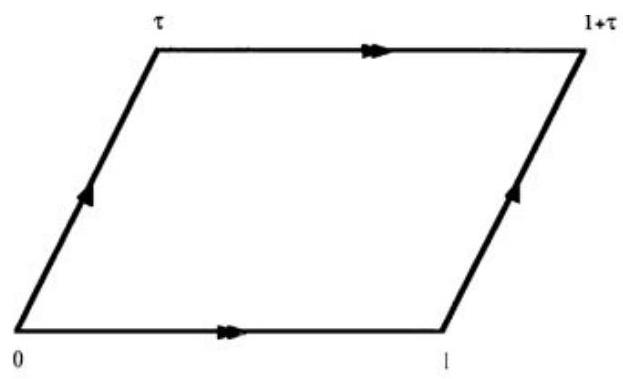
\includegraphics[max width=0.4\textwidth]{images/bo_d3lj80c601uc738kffi0_49_641_372_623_379_0.jpg}
\caption{亏格为 1 的曲线 \(C \cong \mathbb{C} / (\mathbb{Z} \oplus \mathbb{Z}\tau)\)}
\end{figure}

该商空间与平面三次曲线 \(C_3 \subset \mathbb{P}^2_\mathbb{C}\) 之间的同构由一个全纯映射 \(\varphi: \mathbb{C} \to C_3\) 给出，这是 \(C_3\) 的一种“参数化”。但 \(\varphi\) 不能用有理函数表示（见 (2.2)），并且是无限对一的。这就是复变量的双周期函数理论，它是 19 世纪分析学的支柱之一（例如魏尔斯特拉斯 \(\wp\) 函数、黎曼 \(\theta\) 函数）。

另一个重要的注意点是，不同的周期格点 \(\tau\) 通常会导致不同的曲线。它们在拓扑上都同胚于标准环面 \(S^1 \times S^1\)，但作为代数曲线或复解析曲线，它们并不同构。周期 \(\tau\) 是一个模（modulus），即一个复参数，它控制着固定拓扑对象 \(S^1 \times S^1\) 上的复结构 \(C\) 的变化。

对曲线感兴趣的学生应参考 D. Mumford 的《Curves and their Jacobians》，其第一部分较为通俗，或 C. H. Clemens 的《A Scrapbook of Complex Curve Theory》。

\begin{center}
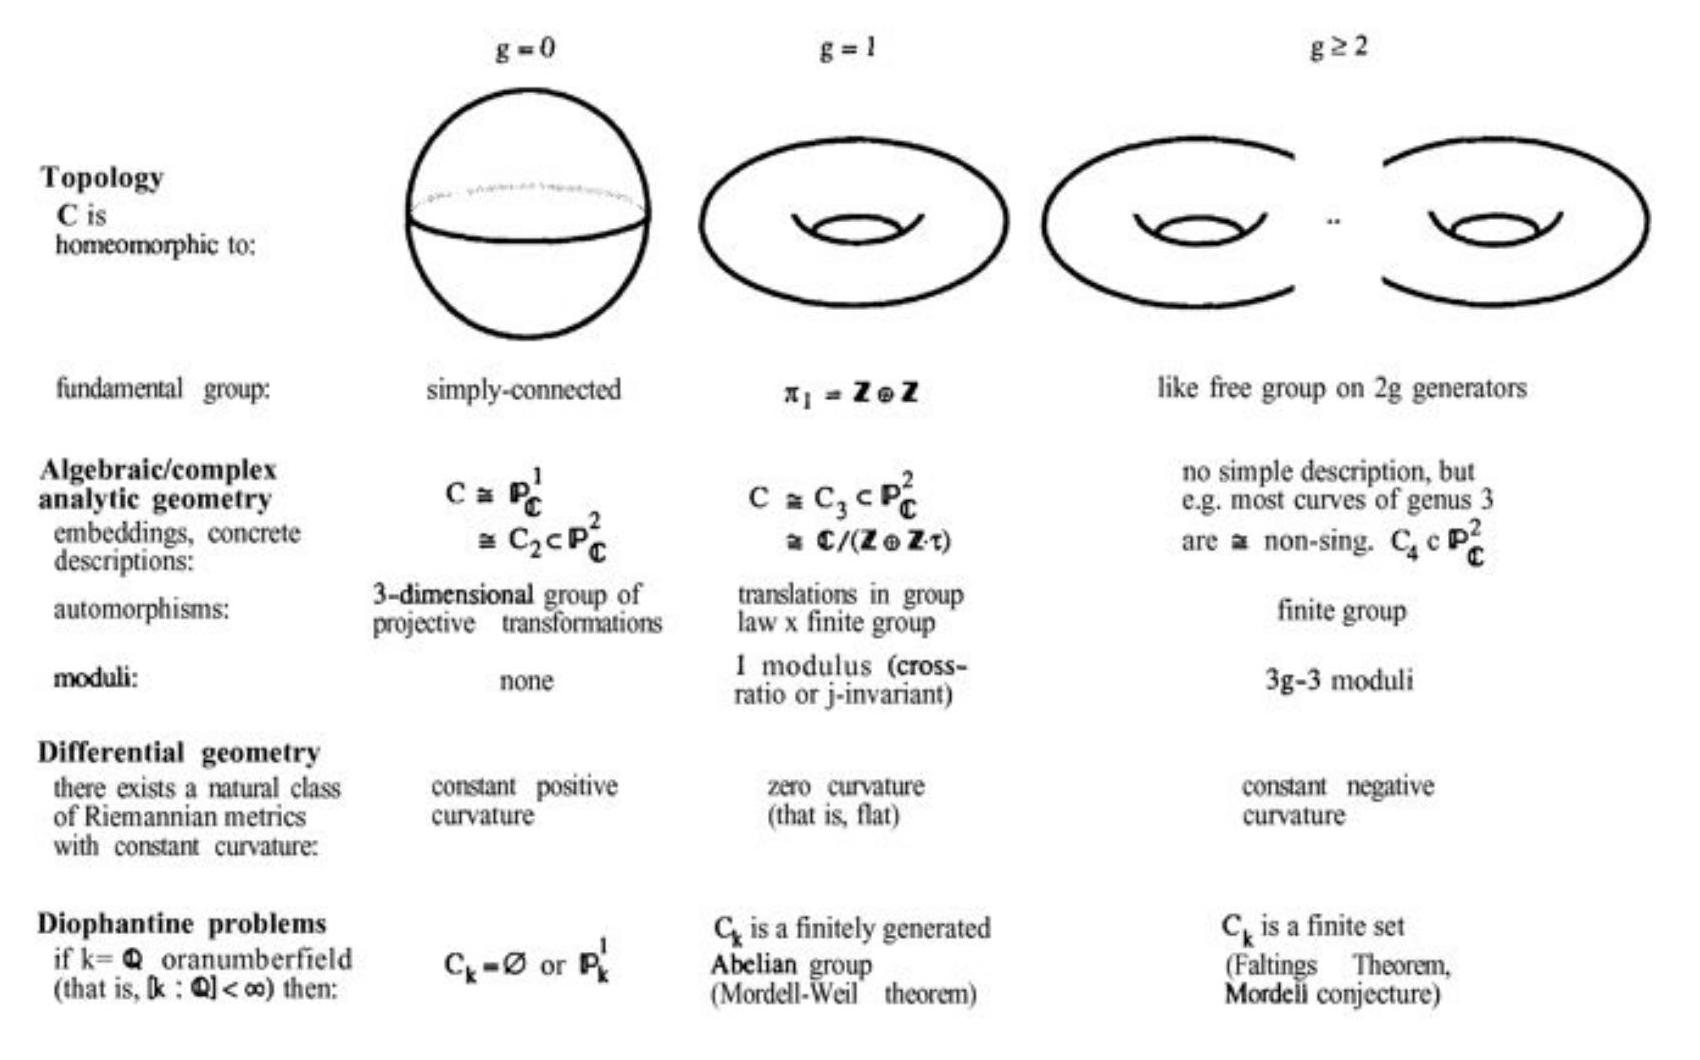
\includegraphics[max width=0.8\textwidth]{images/bo_d3lj80c601uc738kffi0_50_333_253_1060_1700_-1.jpg}
\end{center}
\hspace*{3em}

\part{仿射簇之范畴}

\chapter{仿射簇与零点定理}

本章前半部分主要涉及纯粹的交换代数.请注意，在本笔记中，“环”均指有单位元的交换环.由于本课程并非主讲交换代数，我将略去若干证明细节.

\section{诺特环}

\begin{proposition}[诺特环的等价定义]
对于一个环 \(A\)，以下条件是等价的：
\begin{enumerate}
    \item 环 \(A\) 的每个理想 \(I\) 都是有限生成的.即，对任意理想 \(I \subset A\)，都存在 \({f}_{1},\ldots ,{f}_{k} \in I\) 使得 \(I = \left( {{f}_{1},\ldots ,{f}_{k}}\right)\).
    \item \(A\) 的任意理想升链
    \[
    {I}_{1} \subset  {I}_{2} \subset  \cdots  \subset  {I}_{m} \subset  \cdots
    \]
    最终都会稳定.即，存在一个整数 \(N\)，使得对所有 \(m \geq N\)，都有 \({I}_{m} = {I}_{N}\).这个性质被称为升链条件（Ascending Chain Condition, a.c.c.）.
    \item \(A\) 的任意非空理想集合都存在极大元.
\end{enumerate}
\end{proposition}
\begin{definition}[诺特环]
满足上述等价条件的环 \(A\) 称为诺特环（Noetherian ring）.
\end{definition}

\begin{proof}
(i) \(\Rightarrow\) (ii)：给定一个理想升链 \({I}_{1} \subset  {I}_{2} \subset  \cdots\)，令 \(I = \bigcup_{m=1}^{\infty} {I}_{m}\).不难验证 \(I\) 也是一个理想.根据条件 (i)，\(I\) 是有限生成的，设 \(I = \left( {{f}_{1},\ldots ,{f}_{k}}\right)\).由于每个生成元 \({f}_{i}\) 都属于某个 \({I}_{{m}_{i}}\)，我们取 \(N = \max \left\{ {m}_{1}, \ldots, {m}_{k} \right\}\)，则所有生成元都属于 \({I}_{N}\)，因此 \(I \subset {I}_{N}\).又因为 \({I}_{N} \subset I\)，所以 \(I = {I}_{N}\).这意味着该理想链在第 \(N\) 项后稳定下来，即对所有 \(m \geq N\)，\({I}_{m} = {I}_{N}\).

(ii) \(\Rightarrow\) (iii)：这部分是显然的.（严格来说，它依赖于选择公理.）

(iii) \(\Rightarrow\) (i)：令 \(I\) 为 \(A\) 的任意理想.考虑 \(I\) 中所有有限生成子理想构成的集合 \(\Sigma = \{ J \mid J \subset I \text{ 且 } J \text{ 是有限生成的} \}\).\(\Sigma\) 非空（因为 \((0)\) 在其中）.根据条件 (iii)，\(\Sigma\) 存在一个极大元，记为 \({J}_{0}\).我们断言 \({J}_{0} = I\).如果不然，则存在元素 \(f \in I \setminus {J}_{0}\).此时，理想 \({J}_{0} + Af\) 仍然是有限生成的，并且严格大于 \({J}_{0}\)，这与 \({J}_{0}\) 的极大性矛盾.因此，必有 \({J}_{0} = I\)，即 \(I\) 是有限生成的.
\end{proof}

作为练习，请证明 \(\mathbb{Z}\) 和 \(k\left\lbrack  X\right\rbrack\) 都是诺特环.

\begin{proposition}
(i) 设 \(A\) 为诺特环，\(I \subset  A\) 为其理想，则商环 \(B = A/I\) 也是诺特环.

(ii) 设 \(A\) 为诺特整环，\(K\) 为其分式域.设 \(S \subset A\) 为一个不含0的子集，定义环的局部化
\[
B = A\left\lbrack  {S}^{-1}\right\rbrack   = \left\{  {\left. {\frac{a}{b} \in  K}\right| \; a \in  A, \text{ 且 } b \text{ 是1或S中元素的乘积} }\right\}  .
\]
则 \(B\) 也是诺特环.
\end{proposition}

\begin{proof}
练习：在上述两种情形下，\(B\) 的理想都可以通过 \(A\) 的理想来刻画.具体提示见习题3.4.
\end{proof}

\begin{theorem}[希尔伯特基定理]
若环 \(A\) 是诺特环，则其上的多项式环 \(A\left\lbrack  X\right\rbrack\) 也是诺特环.
\end{theorem}

\begin{proof}
设 \(J \subset  A\left\lbrack  X\right\rbrack\) 为任意理想，我们需要证明 \(J\) 是有限生成的.对任意整数 \(n \geq 0\)，定义 \(J\) 中多项式的首项系数集合：
\[
{I}_{n} = \left\{  {a \in  A\mid {\;\exists f = a{X}^{n} + \cdots \in  J, \deg(f)=n}}\right\} \cup \{0\} .
\]
不难验证，每个 \({I}_{n}\) 都是 \(A\) 的理想，并且它们构成一个升链 \({I}_{0} \subset  {I}_{1} \subset  \cdots\).由于 \(A\) 是诺特环，此升链必在某处稳定，即存在 \(N\) 使得对所有 \(n \geq N\)，都有 \({I}_{n} = {I}_{N}\).

现在我们来构造 \(J\) 的一组生成元.对每个 \(i \in \{0, 1, \ldots, N\}\)，由于 \({I}_{i}\) 是诺特环 \(A\) 中的理想，它是有限生成的.设 \({I}_{i} = ({a}_{i,1},\ldots ,{a}_{i,m_i})\).对每个生成元 \({a}_{i,j}\)，我们从 \(J\) 中选取一个次数为 \(i\) 且首项系数为 \({a}_{i,j}\) 的多项式，记为 \({f}_{i,j}\).

我们断言，集合 \(\mathcal{F} = \left\{  {{f}_{i,j} \mid  i = 0,\ldots ,N, j = 1,\ldots ,{m}_{i}}\right\}\) 是理想 \(J\) 的一组生成元.
令 \(\langle\mathcal{F}\rangle\) 表示由 \(\mathcal{F}\) 生成的理想.我们用归纳法证明对任意 \(g \in J\)，都有 \(g \in \langle\mathcal{F}\rangle\).
设 \(\deg g = m\).
若 \(m > N\)，\(g\) 的首项系数 \(b \in I_m = I_N\).因此 \(b\) 可以写成 \(I_N\) 的生成元的线性组合：\(b = \sum_{j=1}^{m_N} c_j a_{N,j}\)，其中 \(c_j \in A\).构造多项式 \(g_1 = g - \sum_{j=1}^{m_N} c_j X^{m-N} f_{N,j}\).\(g_1\) 依然属于 \(J\)，且其次数严格小于 \(m\).
若 \(m \leq N\)，\(g\) 的首项系数 \(b \in I_m\).因此 \(b = \sum_{j=1}^{m_m} c_j a_{m,j}\).构造多项式 \(g_1 = g - \sum_{j=1}^{m_m} c_j f_{m,j}\).\(g_1\) 依然属于 \(J\)，且其次数严格小于 \(m\).

通过重复这个过程，我们可以不断降低多项式的次数，最终可以把 \(g\) 表示为 \({f}_{i,j}\) 的多项式组合.因此，\(\mathcal{F}\) 生成了 \(J\).
\end{proof}

\begin{corollary}
域 \(k\) 上的任意有限生成代数都是诺特环.
\end{corollary}
\begin{proof}
一个有限生成的 \(k\)-代数是指形如 \(A = k\left\lbrack  {{a}_{1},\ldots ,{a}_{n}}\right\rbrack\) 的环，它由 \(k\) 和元素 \({a}_{1},\ldots ,{a}_{n}\) 作为环生成.显然，任何这样的环都同构于一个多项式环的商环，即 \(A \cong  k\left\lbrack  {{X}_{1},\ldots ,{X}_{n}}\right\rbrack  /I\).
域本身是诺特环.通过对希尔伯特基定理进行归纳，可知 \(k\left\lbrack  {{X}_{1},\ldots ,{X}_{n}}\right\rbrack\) 是诺特环.最后，根据命题3.2(i)，诺特环的商环仍然是诺特环.
\end{proof}

\section{V-I 对应}

设 \(k\) 为任意域，\(A = k\left\lbrack  {{X}_{1},\ldots ,{X}_{n}}\right\rbrack\).遵循代数几何学家的普遍习惯\customfootnote{严格来说，\({\mathbb{A}}^{n}\) 被视为一个代数簇，而 \({k}^{n}\) 仅仅是一个点的集合.如果愿意，可以暂时将此看作一种讲究.详见下文(4.6)及(8.3).}，我们用 \({\mathbb{A}}_{k}^{n}\) 表示 \(k\) 上的 \(n\) 维仿射空间，它作为点集与 \({k}^{n}\) 相同.给定多项式 \(f\left( {{X}_{1},\ldots ,{X}_{n}}\right)  \in A\) 和点 \(P = \left( {{a}_{1},\ldots ,{a}_{n}}\right)  \in  {\mathbb{A}}_{k}^{n}\)，值 \(f\left( P \right) = f\left( {{a}_{1},\ldots ,{a}_{n}}\right)  \in  k\) 被视为“在点 \(P\) 处对函数 \(f\) 求值”.

我们定义一个从理想集到子集的映射：
\[
V: \{ \text{A的理想} \}  \rightarrow  \left\{  {\text{ subsets }X \subset  {\mathbb{A}}_{k}^{n}}\right\}
\]
其定义为
\[
J \mapsto  V\left( J\right)  = \left\{  {P \in  {\mathbb{A}}_{k}^{n} \mid  f\left( P\right)  = 0 \text{ 对所有 } f \in  J}\right\}  .
\]

\begin{definition}[代数集]
子集 \(X \subset  {\mathbb{A}}_{k}^{n}\) 如果是某个理想 \(I\) 的零点集，即 \(X = V\left( I\right)\)，则称其为代数集.
\end{definition}
注意，根据推论3.3，理想 \(I\) 总是有限生成的.如果 \(I = \left( {{f}_{1},\ldots ,{f}_{r}}\right)\)，则
\[
V\left( I\right)  = \left\{  {P \in  {\mathbb{A}}_{k}^{n} \mid  {f}_{i}\left( P\right)  = 0 \text{ 对所有 } i = 1,\ldots ,r}\right\}  ,
\]
因此，代数集就是有限个多项式方程的公共解集.如果 \(I = \left( f\right)\) 是主理想，我们通常用 \(V\left( f\right)\) 代替 \(V\left( I\right)\).这与前两章中记号 \(V : \left( {f = 0}\right)\) 的含义一致.

\section{Zariski拓扑}

\begin{proposition}[Zariski拓扑]
映射 \(V\) 具有以下性质：
\begin{enumerate}
    \item \(V\left( (0) \right)  = {\mathbb{A}}_{k}^{n}\)；\(V\left( A \right)  = \varnothing\).
    \item 若 \(I \subset  J\)，则 \(V\left( I\right)  \supset  V\left( J\right)\).
    \item \(V\left( {{I}_{1} \cap  {I}_{2}}\right)  = V\left( {I}_{1}\right)  \cup  V\left( {I}_{2}\right)\).
    \item \(V\left( {\sum_{{\lambda  \in  \Lambda }}{I}_{\lambda }}\right)  = \bigcap_{{\lambda  \in  \Lambda }}V\left( {I}_{\lambda }\right)\).
\end{enumerate}
因此，\({\mathbb{A}}_{k}^{n}\) 的所有代数子集构成了 \({\mathbb{A}}_{k}^{n}\) 上的一个拓扑的闭集.这个拓扑被称为Zariski拓扑.
\end{proposition}

\begin{proof}
上述性质大多是直接的.对于(iii)中的包含关系 \(V\left( {I}_{1}\right)  \cup  V\left( {I}_{2}\right) \subset V\left( {{I}_{1} \cap  {I}_{2}}\right)\)，证明如下：假设 \(P \notin  V\left( {I}_{1}\right)  \cup  V\left( {I}_{2}\right)\).这意味着存在 \(f \in  {I}_{1}\) 和 \(g \in  {I}_{2}\) 使得 \(f\left( P\right)  \neq  0\) 且 \(g\left( P\right)  \neq  0\).因此，乘积 \({fg} \in  {I}_{1} \cap  {I}_{2}\)，但 \({fg}\left( P\right) = f(P)g(P) \neq  0\)，所以 \(P \notin  V\left( {{I}_{1} \cap  {I}_{2}}\right)\).
\end{proof}

\({\mathbb{A}}_{k}^{n}\) 上的Zariski拓扑可以在任意代数集 \(X \subset  {\mathbb{A}}_{k}^{n}\) 上诱导出子空间拓扑：\(X\) 的闭子集就是 \(X\) 的代数子集.

需要注意的是，簇上的Zariski拓扑非常“弱”，与我们熟悉的度量空间（如 \({\mathbb{R}}^{n}\)）上的拓扑截然不同.例如，在 \({\mathbb{A}}_{k}^{1}\) 中，Zariski闭集只有两种可能：整个 \({\mathbb{A}}_{k}^{1}\) 或有限点集.当 \(k = \mathbb{R}\) 或 \(\mathbb{C}\) 时，由于多项式函数是连续的，Zariski闭集在通常的（度量）拓扑下也是闭集.实际上，Zariski开集或闭集是非常特殊的：\({\mathbb{R}}^{n}\) 上的非空Zariski开集是一个真代数子集的补集，因此它在 \({\mathbb{R}}^{n}\) 中必然是稠密的.

Zariski拓扑可能会让初学者感到困惑.但由于它主要作为一种方便的语言使用，其技术细节很少成为障碍，所以困难更多是心理上的.

\section{I-V 对应}

作为 \(V\) 映射的逆向操作，我们定义一个从子集到理想的映射：
\[
I: \left\{  {\text{子集 }X \subset  {\mathbb{A}}_{k}^{n}}\right\} \to \{ \text{A的理想} \}
\]
其定义为
\[
X \mapsto I\left( X\right)  = \{ f \in  k\left\lbrack  X_1, \ldots, X_n \right\rbrack   \mid  f\left( P\right)  = 0 \text{ 对所有 } P \in  X\} .
\]
即，\(I(X)\) 是在子集 \(X\) 上恒为零的所有多项式构成的理想.

\begin{proposition}
(a) 若 \(X \subset  Y\)，则 \(I\left( X\right)  \supset  I\left( Y\right)\).

(b) 对任意子集 \(X \subset  {\mathbb{A}}_{k}^{n}\)，有 \(X \subset  V\left( {I\left( X\right) }\right)\).等号成立当且仅当 \(X\) 是一个代数集.

(c) 对任意理想 \(J \subset  A\)，有 \(J \subset  I\left( {V\left( J\right) }\right)\).此处的包含关系可能是严格的.
\end{proposition}

\begin{proof}
(a) 是直接的.
(b) 和 (c) 中的包含关系是同义反复：如果 \(I(X)\) 定义为在 \(X\) 上所有点都为零的函数集合，那么对于 \(X\) 中的任意一点，\(I(X)\) 中的所有函数在该点自然都为零.

(b) 的后半部分：如果 \(X = V\left( {I\left( X\right) }\right)\)，那么根据定义，\(X\) 是一个代数集.反之，如果 \(X = V\left( {J_0}\right)\) 是一个代数集，那么根据定义有 \(J_0 \subset I(X)\)，再由 \(V\) 映射的性质(a)，我们得到 \(V(I(X)) \subset V(J_0) = X\).结合 \(X \subset V(I(X))\)，等号成立.

(c) 中的包含关系 \(J \subset  I\left( {V\left( J\right) }\right)\) 可能严格成立的原因有两种.理解这两点至关重要，因为它们直接引出了零点定理的正确表述.
\end{proof}

\paragraph{例1：代数不闭的域} 假设域 \(k\) 不是代数闭的，并设 \(f \in  k\left\lbrack  X\right\rbrack\) 是一个在 \(k\) 中没有根的非零多项式.考虑理想 \(J = \left( f\right)  \subset  k\left\lbrack  X\right\rbrack\).因为 \(1 \notin  J\)，所以 \(J\) 是一个真理想.但是，
\[
V\left( J\right)  = \left\{  {P \in  {\mathbb{A}}_{k}^{1} \mid  f\left( P\right)  = 0}\right\}   = \varnothing .
\]
因此，\(I\left( {V\left( J\right) }\right) = I(\varnothing) = k\left\lbrack  X\right\rbrack\).所以 \(J \subsetneq I(V(J))\).
一个类似的例子：在 \({\mathbb{R}}^{2}\) 中，多项式 \({X}^{2} + {Y}^{2}\) 定义了唯一的点 \(P = \left( {0,0}\right)\)，所以 \(V\left( {{X}^{2} + {Y}^{2}}\right)  = \{ P\}\).但在 \(\{ P\}\) 上为零的多项式远不止 \({X}^{2} + {Y}^{2}\) 的倍数，实际上 \(I\left( P\right)  = \left( {X,Y}\right)\).

\paragraph{例2：幂次的影响} 对任意 \(f \in  k\left\lbrack  {{X}_{1},\ldots ,{X}_{n}}\right\rbrack\) 和整数 \(a \geq  2\)，\({f}^{a}\) 与 \(f\) 定义了相同的零点集，即 \({f}^{a}\left( P\right)  = 0 \Leftrightarrow  f\left( P\right)  = 0\).所以 \(V\left( {f}^{a}\right)  = V\left( f\right)\).这意味着 \(f \in  I\left( {V\left( {f}^{a}\right) }\right)\)，但通常情况下 \(f \notin  \left( {f}^{a}\right)\).这里的问题在于，点集本身无法记录“重数”信息.例如，\({X}^{2} = 0\) 定义的“重线”，其点集与 \({X} = 0\) 定义的直线完全相同.

\section{不可约代数集}

\begin{definition}[不可约]
一个代数集 \(X \subset  {\mathbb{A}}_{k}^{n}\) 是不可约的，如果它不能表示为两个严格的代数子集的并集，即不存在
\[
X = {X}_{1} \cup  {X}_{2}\text{，其中 }\;{X}_{1},{X}_{2} \text{ 是代数集且 } {X}_{1} \neq X, {X}_{2} \neq X.
\]
\end{definition}
例如，代数子集 \(V\left( {xy}\right)  \subset  {\mathbb{A}}_{k}^{2}\) 是两条坐标轴的并，即 \(V\left( x\right) \cup V\left( y\right)\)，因此它是可约的.

\begin{proposition}
(a) 设 \(X \subset  {\mathbb{A}}_{k}^{n}\) 是一个代数集，\(I\left( X\right)\) 是其对应的理想，则
\[
X\text{ 不可约 } \Leftrightarrow  I\left( X\right) \text{ 是素理想.}
\]

(b) 任何代数集 \(X\) 都可以唯一地表示为不可约代数子集的并：
\[
X = {X}_{1} \cup  \cdots  \cup  {X}_{r}
\]
其中每个 \({X}_{i}\) 都是不可约的，且对于 \(i \neq  j\)，\({X}_{i} \not\subset {X}_{j}\).这些 \({X}_{i}\) 被称为 \(X\) 的不可约分量.
\end{proposition}

\begin{proof}
(a) 我们证明 \(X\) 可约当且仅当 \(I(X)\) 不是素理想.

\(\left(  \Rightarrow  \right)\) 假设 \(X = {X}_{1} \cup  {X}_{2}\)，其中 \({X}_{1},{X}_{2}\) 是 \(X\) 的严格代数子集.因为 \({X}_{1} \neq X\)，所以 \(I(X_1) \supsetneq I(X)\)，故存在 \({f}_{1} \in  I\left( {X}_{1}\right)  \setminus  I\left( X\right)\).同理，存在 \({f}_{2} \in  I\left( {X}_{2}\right)  \setminus  I\left( X\right)\).考虑乘积 \({f}_{1}{f}_{2}\).它在 \(X_1\) 和 \(X_2\) 上都为零，因此在 \(X\) 上为零，即 \({f}_{1}{f}_{2} \in  I\left( X\right)\).但 \({f}_{1}, {f}_{2}\) 都不在 \(I(X)\) 中，所以 \(I\left( X\right)\) 不是素理想.

\(\left(  \Leftarrow  \right)\) 假设 \(I\left( X\right)\) 不是素理想，则存在 \({f}_{1},{f}_{2} \notin  I\left( X\right)\) 使得 \({f}_{1}{f}_{2} \in  I\left( X\right)\).令 \({I}_{1} = I\left( X\right) + ({f}_{1})\) 和 \({X}_{1} = V\left( {I}_{1}\right)\).显然 \({X}_{1} \subsetneq  X\).同理，令 \({I}_{2} = I\left( X\right) + ({f}_{2})\) 和 \({X}_{2} = V\left( {I}_{2}\right)\)，则 \({X}_{2} \subsetneq  X\).但是，对任意 \(P \in  X\)，由于 \({f}_{1}{f}_{2}\left( P\right)  = 0\)，必有 \({f}_{1}\left( P\right)  = 0\) 或 \({f}_{2}\left( P\right)  = 0\).这意味着 \(P \in X_1\) 或 \(P \in X_2\).因此 \(X \subset  {X}_{1} \cup  {X}_{2}\).由于 \(X_1, X_2\) 都是 \(X\) 的子集，我们得到 \(X = X_1 \cup X_2\)，故 \(X\) 是可约的.

(b) 首先，我们注意到 \({\mathbb{A}}_{k}^{n}\) 的代数子集满足降链条件（d.c.c.），即任意代数子集的降链
\[
{X}_{1} \supset  {X}_{2} \supset  \cdots  \supset  {X}_{m} \supset  \cdots
\]
最终都会稳定.这是因为对应的理想升链 \(I\left( {X}_{1}\right)  \subset  I\left( {X}_{2}\right)  \subset  \cdots\) 在诺特环 \(A\) 中必定稳定，从而 \(V(I(X_N)) = V(I(X_{N+1}))\)，即 \({X}_{N} = {X}_{N + 1} = \cdots\).
降链条件等价于任何非空代数子集族都存在极小元.

现在来证明(b)的存在性.假设存在某个代数集不能被分解为有限个不可约子集的并，令 \(\Sigma\) 为所有这类代数集的集合.若 \(\Sigma\) 非空，则其中必有一个极小元 \(X\).
\(X\) 本身不可能是不可约的，否则它就不是 \(\Sigma\) 的成员.
因此 \(X\) 必然是可约的，即 \(X = {X}_{1} \cup  {X}_{2}\)，其中 \({X}_{1},{X}_{2}\) 是 \(X\) 的严格子集.根据 \(X\) 的极小性，\({X}_{1}\) 和 \({X}_{2}\) 都不在 \(\Sigma\) 中，所以它们都可以被分解为有限个不可约子集的并.将这两个分解合并，就得到了 \(X\) 的一个分解，这与 \(X \in \Sigma\) 矛盾.因此 \(\Sigma\) 必须为空.
唯一性是一个简单的练习，见习题3.8.
\end{proof}

这个证明是典型的代数风格：逻辑严密但可能掩盖了直观.其核心思想是，如果一个代数集是可约的，就分解它；然后对分解出的部分重复此过程.这个过程必须在有限步内终止，否则将构造出一个无限的严格降链，与降链条件矛盾.

\section{零点定理的准备工作}

现在我们来陈述并证明零点定理（Nullstellensatz）.任何版本的证明都有其难点，我选择将其分为两部分.首先，我将陈述一个交换代数中的重要结论，其证明（具有强烈的几何内涵）将在(3.15)节给出.

\begin{lemma}[Zariski引理]
设 \(k\) 为一个域，\(A\) 是 \(k\) 上的一个有限生成代数.若 \(A\) 本身也是一个域，则 \(A\) 是 \(k\) 的一个有限代数扩张.
\end{lemma}

为了粗略地说明其合理性，注意如果 \(t \in  A\) 在 \(k\) 上是超越的，那么 \(k\left\lbrack  t\right\rbrack\) 是一个多项式环，它有无穷多个素理想（由欧几里得证明可知）.可以证明，这意味着 \(k(t)\) 作为 \(k\)-代数不是有限生成的：有限个有理函数 \({p}_{i}/{q}_{i} \in  k\left( t\right)\) 的分母中只涉及有限个素理想.

\section{根理想}

\begin{definition}[根理想]
若 \(I\) 是环 \(A\) 的一个理想，则 \(I\) 的根（radical）定义为
\[
\operatorname{rad}(I) = \sqrt{I} = \left\{  {f \in  A \mid  {f}^{n} \in  I \text{ 对某个整数 } n>0}\right\}  .
\]
\end{definition}
\(\sqrt{I}\) 本身也是一个理想.一个理想 \(I\) 如果满足 \(I = \sqrt{I}\)，则称其为根理想.
注意，素理想都是根理想.在唯一分解整环（如 \(k\left\lbrack  {{X}_{1},\ldots ,{X}_{n}}\right\rbrack\)）中，一个主理想 \(I = \left( f\right)\)（其中 \(f = \prod {f}_{i}^{{n}_{i}}\) 是 \(f\) 的素因子分解）的根理想是 \(\sqrt{I} = \left( {f}_{\text{red}}\right)\)，其中 \({f}_{\text{red}} = \prod {f}_{i}\) 是 \(f\) 的约化部分.

\begin{theorem}[希尔伯特零点定理]
设 \(k\) 为一个代数闭域，\(A = k\left\lbrack  {{X}_{1},\ldots ,{X}_{n}}\right\rbrack\).
\begin{enumerate}
    \item[\upshape (a)] \(A\) 的每个极大理想都具有 \({m}_{P} = \left( {{X}_{1} - {a}_{1},\ldots ,{X}_{n} - {a}_{n}}\right)\) 的形式，对应于某个点 \(P = \left( {{a}_{1},\ldots ,{a}_{n}}\right)  \in  {\mathbb{A}}_{k}^{n}\).换言之，极大理想就是由所有在某点 \(P\) 处为零的函数构成的理想 \(I(P)\).
    \item[\upshape (b)] (弱零点定理) 设 \(J \subset  A\) 是一个真理想（即 \(J \neq A\)），则其零点集 \(V\left( J\right)\) 非空.
    \item[\upshape (c)] (强零点定理) 对任意理想 \(J \subset  A\)，
    \[
    I\left( {V\left( J\right) }\right)  = \sqrt{J}.
    \]
\end{enumerate}
\end{theorem}

该定理的核心是(b)，它断言只要一个理想不是整个多项式环，它就必然在 \({\mathbb{A}}_{k}^{n}\) 中有公共零点.注意，如果 \(k\) 不是代数闭的，(b)就不成立.定理的德语名称（Nullstelle = 零点，Satz = 定理）有助于记忆其内容.

\begin{corollary}
在代数闭域 \(k\) 上，映射 \(V\) 和 \(I\) 建立了在 \({\mathbb{A}}_{k}^{n}\) 的根理想与代数子集之间的一一对应关系.
\end{corollary}
\begin{proof}
对任意代数集 \(X\)，我们有 \(V\left( {I\left( X\right) }\right)  = X\).对任意根理想 \(J\)，根据零点定理(c)，我们有 \(I\left( {V\left( J\right) }\right)  = J\).
\end{proof}

\begin{proof}[零点定理的证明 (假设Zariski引理)]
(a) 设 \(m \subset  k\left\lbrack  {{X}_{1},\ldots ,{X}_{n}}\right\rbrack\) 是一个极大理想.令 \(K = k\left\lbrack  {{X}_{1},\ldots ,{X}_{n}}\right\rbrack  /m\).由于 \(m\) 是极大理想，\(K\) 是一个域.同时，\(K\) 是一个有限生成的 \(k\)-代数（由 \({X}_{i}\) 在商环中的像生成）.根据Zariski引理(3.8)，\(K\) 是 \(k\) 的一个代数扩张.但 \(k\) 是代数闭的，所以 \(k \to K\) 必然是同构.

这意味着，对每个 \(i\)，\({X}_{i}\) 在商环中的像 \(\bar{X_i} \in K\) 对应于 \(k\) 中的某个元素 \({a}_{i}\).因此，\({X}_{i} - {a}_{i} \in \ker(k[X_1,\dots,X_n] \to K) = m\).于是，理想 \(\left( {{X}_{1} - {a}_{1},\ldots ,{X}_{n} - {a}_{n}}\right)\) 包含于 \(m\).但前者本身就是一个极大理想，所以两者必须相等.

(a) \(\Rightarrow\) (b) 这很简单.如果 \(J \neq A\)，那么 \(J\) 必然包含于某个极大理想 \(m\) 中（极大理想的存在性由诺特环的升链条件保证）.根据(a)，\(m\) 的形式是 \({m}_{P} = \left( {{X}_{1} - {a}_{1},\ldots ,{X}_{n} - {a}_{n}}\right)\) for some \(P \in {\mathbb{A}}_{k}^{n}\).\(J \subset m_P\) 意味着所有 \(J\) 中的函数在点 \(P\) 处都为零.因此 \(P \in  V\left( J\right)\)，即 \(V(J)\) 非空.

(b) \(\Rightarrow\) (c) 这个证明需要一个巧妙的技巧，称为“拉宾诺维奇的诡计”.设 \(J \subset  k\left\lbrack  {{X}_{1},\ldots ,{X}_{n}}\right\rbrack\) 为任意理想，并设 \(f \in I(V(J))\).这意味着 \(f\) 在 \(V(J)\) 的所有点上都为零.
我们想证明存在某个 \(N>0\) 使得 \({f}^{N} \in  J\).

引入一个新变量 \(Y\)，并考虑环 \(k\left\lbrack  {{X}_{1},\ldots ,{X}_{n},Y}\right\rbrack\) 中的新理想
\[
{J}_{1} = J + \left( {1 - fY}\right)  \subset  k\left\lbrack  {{X}_{1},\ldots ,{X}_{n},Y}\right\rbrack.
\]
\(J_1\) 的零点集 \(V(J_1) \subset {\mathbb{A}}^{n+1}\) 由满足 \(g(P)=0\) 对所有 \(g \in J\) 且 \(1-f(P)b=0\) 的点 \((P,b)\) 构成.第二个条件等价于 \(f(P) \neq 0\).
但我们已知 \(f\) 在 \(V(J)\) 上恒为零，所以不存在这样的点 \((P,b)\).因此 \(V(J_1) = \varnothing\).

由于我们在一个代数闭域上，弱零点定理(b)告诉我们，如果一个理想的零点集为空，那么这个理想必须是整个环.所以 \(J_1 = k\left\lbrack  {{X}_{1},\ldots ,{X}_{n},Y}\right\rbrack\)，即 \(1 \in J_1\).
这意味着存在表达式
\[
1 = \sum_{i} g_i f_i + h(1-fY)
\]
其中 \({f}_{i} \in  J\)，而 \({g}_{i}, h \in  k\left\lbrack  {{X}_{1},\ldots ,{X}_{n},Y}\right\rbrack\).

这个等式是在多项式环 \(k\left\lbrack  {{X}_{1},\ldots ,{X}_{n},Y}\right\rbrack\) 中成立的恒等式.我们可以将它看作在有理函数域 \(k(X_1, \ldots, X_n)\) 中关于变量 \(Y\) 的等式，然后代入 \(Y = 1/f\).这使得 \(1-fY\) 项变为0，我们得到：
\[
1 = \sum_{i} g_i(X_1, \ldots, X_n, 1/f) f_i.
\]
将右边的分母 \(f\) 的幂次全部通分，设最高次幂为 \(f^N\)，我们可以得到
\[
1 = \frac{\sum_i \tilde{g_i} f_i}{f^N}
\]
其中 \(\tilde{g_i} \in k[X_1, \ldots, X_n]\).整理后得到 \({f}^{N} = \sum_i \tilde{g_i} f_i\)，这表明 \({f}^{N} \in  J\).
\end{proof}

\section{例子}

(a) \textbf{超曲面}. 最简单的簇是超曲面 \(V\left( f\right)  : \left( {f = 0}\right)  \subset  {\mathbb{A}}_{k}^{n}\).当 \(k\) 是代数闭域时，不可约多项式 \(f \in  k\left\lbrack  {{X}_{1},\ldots ,{X}_{n}}\right\rbrack\) 与不可约超曲面之间存在一一对应.由零点定理可知，两个不同的不可约多项式（非倍数关系）定义了不同的超曲面.这并非显然（例如，在 \(\mathbb{R}\) 上是错误的），但可以通过更经典的消元理论来证明.

(b) \textbf{需要多个生成元的理想}. 除了超曲面，大多数簇都由“许多”方程定义.与直觉相反，一个簇的理想 \(I\left( X\right)\) 通常需要远多于其“余维数”的生成元.下面是一个例子，一条曲线 \(C \subset  {\mathbb{A}}_{k}^{3}\) 的理想 \(I\left( C\right)\) 需要3个生成元（假设 \(k\) 是无限域）.

考虑参数化曲线 \(C = \{ (t^3, t^4, t^5) \mid t \in k \}\).这是一个不可约曲线.可以证明其理想为
\[ I(C) = (u^3-vw, v^2-uw, w^2-u^2v). \]
这个理想不能由两个元素生成.这个例子属于一类漂亮的“单项式”簇.一般而言，猜测一个簇的不可约分量可能相当棘手，证明它们不可约则更难.

\section{有限代数}

现在我们开始准备证明Zariski引理(3.8).设 \(A \subset  B\) 为环.
\begin{definition}
如果存在有限个元素 \({b}_{1},\ldots ,{b}_{n} \in B\) 使得 \(B = A\left\lbrack  {{b}_{1},\ldots ,{b}_{n}}\right\rbrack\)，则称 \(B\) 是 \(A\) 上的\textbf{有限生成代数}.这意味着 \(B\) 作为环由 \(A\) 和 \({b}_{1},\ldots ,{b}_{n}\) 生成.

如果存在有限个元素 \({b}_{1},\ldots ,{b}_{n} \in B\) 使得 \(B = A{b}_{1} + \cdots  + A{b}_{n}\)，则称 \(B\) 是一个\textbf{有限 \(A\)-模}（或有限 \(A\)-代数）.这意味着 \(B\) 作为 \(A\)-模是有限生成的.
\end{definition}
关键区别在于：作为环生成时，允许生成元的多项式表达式；作为模生成时，只允许线性组合.例如，\(k\left\lbrack  X\right\rbrack\) 是有限生成的 \(k\)-代数（由一个元素 \(X\) 生成），但不是有限 \(k\)-模（因为它作为 \(k\)-向量空间的维数是无限的）.

\begin{proposition}
(i) 设 \(A \subset  B \subset  C\) 为环.若 \(B\) 是有限 \(A\)-模且 \(C\) 是有限 \(B\)-模，则 \(C\) 是有限 \(A\)-模.

(ii) 如果 \(A \subset  B\) 是一个有限 \(A\)-模，则 \(B\) 中的每个元素 \(x\) 都在 \(A\) 上是整的，即 \(x\) 满足一个首一的整系数多项式方程：
\[
{x}^{n} + {a}_{n - 1}{x}^{n - 1} + \cdots  + {a}_{0} = 0\;\text{，其中 }{a}_{i} \in  A.
\]

(iii) 反之，如果 \(x\) 在 \(A\) 上是整的，那么 \(B = A\left\lbrack  x\right\rbrack\) 是一个有限 \(A\)-模.
\end{proposition}

\begin{proof}
(i) 和 (iii) 是简单的练习.对于 (ii)，我们使用一个巧妙的“行列式技巧”：
假设 \(B = \sum_{i=1}^n A{b}_{i}\).对任意 \(x \in B\)，由于 \(x{b}_{i} \in  B\)，它可以表示为基底的线性组合：
\[
x{b}_{i} = \sum_{j=1}^n {a}_{ij}{b}_{j} \quad (a_{ij} \in A)
\]
这可以写成一个矩阵方程 \(\sum_{j=1}^n \left( {x{\delta }_{ij} - {a}_{ij}}\right) {b}_{j} = 0\).令 \(M\) 为矩阵 \((x{\delta }_{ij} - {a}_{ij})\).根据线性代数，我们有 \(\det(M) \cdot b_j = 0\) 对所有 \(j\) 成立.由于 \(1_B \in B\) 是 \(b_j\) 的线性组合，我们得到 \(\det(M) \cdot 1_B = 0\)，即 \(\det(M)=0\).
\(\det(M)\) 展开后就是一个关于 \(x\) 的、系数在 \(A\) 中的首一多项式.
\end{proof}

\section{诺特正规化引理}

\begin{theorem}[诺特正规化引理]
设 \(k\) 是一个无限域，\(A = k\left\lbrack  {{a}_{1},\ldots ,{a}_{n}}\right\rbrack\) 是一个有限生成的 \(k\)-代数.则存在整数 \(m \leq  n\) 和元素 \({y}_{1},\ldots ,{y}_{m} \in  A\) 使得：
\begin{enumerate}
    \item \({y}_{1},\ldots ,{y}_{m}\) 在 \(k\) 上代数无关；
    \item \(A\) 是一个有限 \(k\left\lbrack  {{y}_{1},\ldots ,{y}_{m}}\right\rbrack\)-模.
\end{enumerate}
\end{theorem}

这个定理断言，任何有限生成 \(k\)-代数都可以通过先进行纯超越扩张，然后再进行整扩张得到.

\begin{proof}[证明思路]
考虑满同态 \(\phi: k\left\lbrack  {{X}_{1},\ldots ,{X}_{n}}\right\rbrack   \rightarrow  A\)，其核为 \(I\).如果 \(I=(0)\)，则定理成立.否则，取非零多项式 \(f \in I\).证明的核心是通过对变量 \({X}_{1},\ldots ,{X}_{n}\) 做一个线性变换，使得 \(f\) 变成一个关于某个新变量（比如 \(X_n\)）的首一多项式，其系数是关于其他 \(n-1\) 个新变量的多项式.
具体来说，令 \({X}_{i}' = {X}_{i} - {\alpha }_{i}{X}_{n}\) for \(i=1, \ldots, n-1\).对于恰当选择的 \({\alpha }_{i} \in  k\)，多项式 \(f(X_1'+\alpha_1 X_n, \ldots, X_{n-1}'+\alpha_{n-1}X_n, X_n)\) 是一个关于 \(X_n\) 的首一多项式.
这表明 \(a_n\) 在子代数 \(A' = k[a_1', \ldots, a_{n-1}']\) 上是整的，其中 \(a_i' = \phi(X_i')\).因此 \(A\) 是一个有限 \(A'\)-模.
然后对 \(A'\) 应用归纳假设即可完成证明.
\end{proof}

\paragraph{几何意义} 诺特正规化引理在几何上对应于一个有限的、满的线性投影.设 \(V \subset {\mathbb{A}}^n\) 是一个代数簇.引理表明，总存在一个到某个低维仿射空间 \({\mathbb{A}}^m\) 的投影 \(\pi: V \to {\mathbb{A}}^m\)，使得这个投影是有限满射（即每个点的纤维都是有限非空的）.

\section{Zariski引理的证明}

现在我们利用诺特正规化引理来证明Zariski引理(3.8).
设 \(A = k\left\lbrack  {{a}_{1},\ldots ,{a}_{n}}\right\rbrack\) 是一个有限生成的 \(k\)-代数，且 \(A\) 是一个域.
根据诺特正规化引理，存在代数无关的元素 \({y}_{1},\ldots ,{y}_{m} \in  A\)，使得 \(A\) 是多项式环 \(B = k\left\lbrack  {{y}_{1},\ldots ,{y}_{m}}\right\rbrack\) 上的一个有限模.

我们有如下引理：
\begin{lemma}
如果 \(A\) 是一个域，且 \(B \subset  A\) 是一个子环，使得 \(A\) 是一个有限 \(B\)-模，则 \(B\) 也是一个域.
\end{lemma}
\begin{proof}[引理的证明]
对任意非零元素 \(b \in B\)，其逆元 \({b}^{-1}\) 存在于域 \(A\) 中.由于 \(A\) 是有限 \(B\)-模，\({b}^{-1}\) 在 \(B\) 上是整的.即存在关系
\[
{b}^{-n} + {a}_{n - 1}{b}^{-(n - 1)} + \cdots  + {a}_{1}{b}^{-1} + {a}_{0} = 0,\;\text{ 其中 }{a}_{i} \in  B.
\]
两边同乘以 \({b}^{n - 1}\)，整理可得
\[
{b}^{-1} =  - \left( {{a}_{n - 1} + {a}_{n - 2}b + \cdots  + {a}_{0}{b}^{n - 1}}\right).
\]
由于右边所有项都在 \(B\) 中，所以 \({b}^{-1} \in B\).因此 \(B\) 是一个域.
\end{proof}

回到Zariski引理的证明.我们已经知道 \(B = k\left\lbrack  {{y}_{1},\ldots ,{y}_{m}}\right\rbrack\) 是一个域.但一个多项式环只有在 \(m=0\) 且 \(k\) 是域时才是域.因此 \(m=0\)，这意味着 \(B=k\).
于是，\(A\) 是 \(k\) 上的一个有限模，即 \(A\) 是 \(k\) 的一个有限维向量空间.所以 \(A\) 是 \(k\) 的一个有限代数扩张.Zariski引理证毕，从而完成了零点定理的全部证明.

\section{可分性附录}

为了确保论证在特征 \(p>0\) 时依然有效，需要一些关于可分扩张的额外考虑.
在诺特正规化引理的叙述中，如果 \(A\) 是一个整环，我们可以选择 \({y}_{1},\ldots ,{y}_{m}\) 使得 \(A\) 的分式域 \(K\) 是 \(k\left( {{y}_{1},\ldots ,{y}_{m}}\right)\) 的一个可分扩张.这在后续推导“每个簇都双有理等价于一个超曲面”时会用到.

\section{归约到超曲面}

回顾伽罗瓦理论中的本原元定理：
\begin{theorem}[本原元定理]
设 \(K\) 是无限域，\(L/K\) 是有限可分域扩张，则存在 \(x \in  L\) 使得 \(L = K\left( x\right)\).
\end{theorem}

结合诺特正规化引理和本原元定理，我们可以得到以下推论：
\begin{corollary}
对任意有限生成 \(k\)-代数 \(A\)（整环），其分式域 \(K\) 可以表示为 \(K = k(y_1, \ldots, y_m, y_{m+1})\)，其中 \(y_1, \ldots, y_m\) 在 \(k\) 上代数无关，而 \(y_{m+1}\) 在 \(k(y_1, \ldots, y_m)\) 上是代数的.
\end{corollary}
从代数角度看，这意味着任何有限生成的域扩张都可以分解为一个纯超越扩张，再跟一个单代数扩张.这个结果的几何意义是：任何不可约簇都双有理等价于一个超曲面.具体将在第5章阐明.

\section{第三章习题}

3.1 一个整环 \(A\) 是主理想整环(PID)，如果 \(A\) 的每个理想都是主理想.请直接证明PID满足升链条件.

3.2 证明一个整环 \(A\) 是唯一分解整环(UFD)当且仅当每个主理想的升链稳定，且 \(A\) 的每个不可约元都是素元.

3.3 (i) 证明高斯引理. (ii) 利用高斯引理和归纳法证明，若 \(k\) 是UFD，则 \(k\left\lbrack  {{X}_{1},\ldots ,{X}_{n}}\right\rbrack\) 也是UFD.

3.4 证明命题3.2(ii)：证明环的局部化 \(A[S^{-1}]\) 的理想与其在 \(A\) 中的“收缩”有一一对应关系，并由此推断若 \(A\) 是诺特环，则 \(A[S^{-1}]\) 也是诺特环.

3.5 设 \(J = \left( {{XY},{XZ},{YZ}}\right)  \subset  k\left\lbrack  {X,Y,Z}\right\rbrack\).求 \(V\left( J\right)  \subset  {\mathbb{A}}^{3}\).它是不可约的吗？\(J = I\left( {V\left( J\right) }\right)\) 是否成立？证明 \(J\) 不能由两个元素生成.现在设 \({J}^{\prime } = \left( {{XY},\left( {X - Y}\right) Z}\right)\).求 \(V\left( {J}^{\prime }\right)\)，并计算 \(\sqrt{J^{\prime}}\).

3.6 设 \(J = \left( {{X}^{2} + {Y}^{2} - 1,Y - 1}\right)\).求一个多项式 \(f \in  I\left( {V\left( J\right) }\right)  \setminus  J\).

3.7 设 \(J = \left( {{X}^{2} + {Y}^{2} + {Z}^{2},{XY} + {XZ} + {YZ}}\right)\).确定 \(V\left( J\right)\) 和 \(I\left( {V\left( J\right) }\right)\).

3.8 证明代数集的不可约分量分解是唯一的（在不计顺序的意义下）.

3.9 设 \(f = {X}^{2} - {Y}^{2}\) 和 \(g = {X}^{3} + X{Y}^{2} - {Y}^{3} - {X}^{2}Y - X + Y\).求 \(V\left( {f,g}\right)  \subset  {\mathbb{A}}_{\mathbb{C}}^{2}\) 的不可约分量.

3.10 若 \(J = \left( {{uw} - {v}^{2},{w}^{3} - {u}^{5}}\right)\) ，证明 \(V\left( J\right)\) 有两个不可约分量，其中一个是(3.11, b)中的曲线 \(C\) .

证明同一曲线 \(C\) 可以由两个方程 \({uw} = {v}^{2}\) 和 \({u}^{5} - 2{u}^{2}{vw} + {w}^{3} =\) 0定义.这里的关键是第二个方程，在限制于二次锥面 \(\left( {{uw} = {v}^{2}}\right)\) 时，试图成为一个平方.

3.11 设 \(f = {v}^{2} - {uw},g = {u}^{4} - {vw},h = {w}^{2} - {u}^{3}v\) .按照(3.11, b)的思路确定簇 \(V\left( {f,g,h}\right)  \subset  {\mathbb{A}}^{3}\) .找出 \(V\left( {f,g}\right) ,V\left( {f,h}\right)\) 和 \(V\left( {g,h}\right)\) 是否还有其他有趣的分量.

3.12 (i) 证明对于任意域 \(k\) ， \({\mathbb{A}}_{k}^{1}\) 中的代数集要么是有限的，要么是整个 \({\mathbb{A}}_{k}^{1}\) .由此推断Zariski拓扑是余有限拓扑.

(ii) 设 \(k\) 为任意域， \(f,g \in  k\left\lbrack  {X,Y}\right\rbrack\) 为不可约元素，且彼此不互为倍数.证明 \(V\left( {f,g}\right)\) 是有限的.[提示:写出 \(K = k\left( X\right)\) ；首先证明在PID \(K\left\lbrack  Y\right\rbrack\) 中 \(f,g\) 没有公因子.由此推断存在 \(p,q \in  K\left\lbrack  Y\right\rbrack\) 使得 \({pf} + {qg} = 1\) ；现在通过清除 \(p,q\) 中的分母，证明存在 \(h \in  k\left\lbrack  X\right\rbrack\) 和 \(a,b \in  k\left\lbrack  {X,Y}\right\rbrack\) 使得 \(h = {af} + {bg}\) .因此得出 \(V\left( {f,g}\right)\) 中点的 \(X\) 坐标只有有限多种可能值.]

(iii) 证明任意代数集 \(V \subset  {\mathbb{A}}_{k}^{2}\) 是有限个点和曲线的并.

3.13 (a) 设 \(k\) 为无限域， \(f \in  k\left\lbrack  {{X}_{1},\ldots ,{X}_{n}}\right\rbrack\) ；假设 \(f\) 是非常数的，即 \(f \notin  k\) .证明 \(V\left( f\right)  \neq  {\mathbb{A}}_{k}^{n}\) .[提示:假设 \(f\) 涉及 \({X}_{n}\) ，考虑 \(f = \sum {a}_{i}\left( {{X}_{1},\ldots ,{X}_{n - 1}}\right) {X}_{n}^{i}\) ；现在对 \(n\) 使用归纳法.]

(b) 现在假设 \(k\) 是代数闭的，且 \(f\) 如(a)所述.假设 \(f\) 在 \({X}_{n}\) 中的次数为 \(m\) ，其首项为 \({a}_{m}\left( {{X}_{1},\ldots ,{X}_{n - 1}}\right) {X}_{n}^{m}\) ；证明无论 \({a}_{m} \neq  0\) ，对应每个 \(\left( {{X}_{1},\ldots ,{X}_{n - 1}}\right)\) 的值， \(V\left( f\right)\) 中都有有限且非空的点集.特别地，推断如果 \(n \geq  2\) ，则 \(V\left( f\right)\) 是无限的.

(c) 结合(b)和练习3.12(iii)的结果，推断如果域 \(k\) 是代数闭的，则不同的不可约多项式 \(f \in  k\left\lbrack  {X,Y}\right\rbrack\) 定义了 \({\mathbb{A}}_{k}^{2}\) 中不同的超曲面(参见(3.11, a)).

(d) 将(c)的结果推广到 \({\mathbb{A}}_{k}^{n}\) .

3.14 举例说明(3.13)中给出的诺特正规化(Noether normalisation)证明在有限域 \(k\) 上失效的情况.[提示:找到一个多项式 \(f\left( {X,Y}\right)\) ，使得 \({F}_{d}\left( {\alpha ,1}\right)  = {\alpha }^{q} - \alpha\) ，从而对所有 \(\alpha  \in  k\) 都有 \({F}_{d}\left( {\alpha ,1}\right)  = 0\) .]

3.15 设 \(A\) 为环， \(A \subset  B\) 为有限的 \(A\) -代数.证明如果 \(m\) 是 \(A\) 的极大理想，则 \({mB} \neq  B\) .[提示:反证法，假设 \(B = {mB}\) ；若 \(B = \sum A{b}_{i}\) ，则对每个 \(i\) ，有 \({b}_{i} = \sum {a}_{ij}{b}_{j}\) 且 \({a}_{ij} \in  m\) .现在证明

\[
\Delta  = \det \left( {{\delta }_{ij} - {a}_{ij}}\right)  = 0,
\]

并得出 \({1}_{B} \in  m\) ，矛盾.另见[Atiyah 和 Macdonald，命题2.4及推论2.5].

3.16 设 \(A = k\left\lbrack  {{a}_{1},\ldots ,{a}_{n}}\right\rbrack\) 如诺特正规化(3.13)中所述，写作 \(I =\)  \(\ker \left\{  {k\left\lbrack  {{X}_{1},\ldots ,{X}_{n}}\right\rbrack   \rightarrow  k\left\lbrack  {{a}_{1},\ldots ,{a}_{n}}\right\rbrack   = A}\right\}\) ，并考虑 \({\mathbb{A}}_{k}^{n}\) 中的 \(V = V\left( I\right)\) ；为简便起见，假设 \(I\) 为素理想.

设 \({Y}_{1},\ldots ,{Y}_{m}\) 为 \({X}_{1},\ldots ,{X}_{m}\) 中的一般线性形式，写 \(\pi  : {\mathbb{A}}_{k}^{n} \rightarrow  {\mathbb{A}}_{k}^{m}\) 为由 \({Y}_{1},\ldots ,{Y}_{m}\) 定义的线性射影；设 \(p = \pi  \mid  V : V \rightarrow  {\mathbb{A}}_{k}^{m}\) .证明(3.13)中的(i)和(ii)意味着每个 \(P \in  {\mathbb{A}}_{k}^{m},{p}^{-1}\left( P\right)\) 上方是有限集，且当 \(k\) 为代数闭域时非空.[提示: \(I\) 包含每个 \({X}_{i}\) 在 \(k\left\lbrack  {{Y}_{1},\ldots ,{Y}_{m}}\right\rbrack\) 上的首一关系；有限性由此易得.非空性则利用练习3.15证明对任意 \(P = \left( {{b}_{1},\ldots ,{b}_{m}}\right)  \in  {\mathbb{A}}_{k}^{m}\) ，理想 \({J}_{P} = I + \left( {{Y}_{1} - {b}_{1},\ldots ,{Y}_{m} - {b}_{m}}\right)  \neq  k\left\lbrack  {{X}_{1},\ldots ,{X}_{m}}\right\rbrack\) .然后应用Nullstellensatz的非空性断言.]


\chapter{代数簇上的函数}

本章中，我们将在一个固定的域 \(k\) 上进行讨论.从(4.8, II)节开始，我们将假设 \(k\) 是代数闭域.为方便理解，读者不妨始终假设 \(k = \mathbb{C}\)，这在大部分情况下不会影响结论的本质，甚至可能有助于直观把握.为简化符号，我们有时会省略对基域 \(k\) 的提及.

\section{多项式函数}

设 \(V \subset  {\mathbb{A}}_{k}^{n}\) 是一个代数集，其理想为 \(I(V)\).商环 \(k[V] = k[X_1, \ldots, X_n]/I(V)\) 很自然地成为 \(V\) 上的函数环.

具体而言，我们定义 \(V\) 上的\textbf{多项式函数}（polynomial function）为形如 \(f : V \rightarrow  k\) 的映射，其形式为 \(P \mapsto  F(P)\)，其中 \(F \in  k[X_1, \ldots, X_n]\).这意味着 \(f\) 是由某个多项式 \(F : {\mathbb{A}}^{n} \rightarrow  k\) 在 \(V\) 上的限制.

根据理想 \(I(V)\) 的定义，两个多项式 \(F, G \in  k[X_1, \ldots, X_n]\) 在 \(V\) 上定义了相同的函数，当且仅当
\[
F(P) - G(P) = 0 \text{ 对所有 } P \in  V,
\]
即当且仅当 \(F - G \in  I(V)\).因此，我们定义\textbf{坐标环}（coordinate ring）\(k[V]\) 为：
\[
k[V] = \{ f : V \rightarrow  k \mid  f \text{ 是多项式函数} \} \cong  k[X_1, \ldots, X_n]/I(V).
\]
该环是包含所有坐标函数 \(x_i\) 以及常数域 \(k\) 的最小函数环，因此“坐标环”这一传统术语在此处是相当直观的.

\section{\(k[V]\) 与 \(V\) 的代数子集}

一个代数集 \(X \subset  {\mathbb{A}}^{n}\) 包含于 \(V\) 中，当且仅当 \(I(X) \supset  I(V)\).另一方面，\(k[X_1, \ldots, X_n]\) 中包含 \(I(V)\) 的理想与商环 \(k[X_1, \ldots, X_n]/I(V)\) 的理想之间存在着自然的一一对应关系.（具体来说，理想 \(J\) 满足 \(I(V) \subset  J \subset  k[X_1, \ldots, X_n]\) 对应于商环中的理想 \(J/I(V)\)；反之，\(k[X_1, \ldots, X_n]/I(V)\) 的理想 \({J}_{0}\) 对应于它在 \(k[X_1, \ldots, X_n]\) 中的原像.）

因此，在 \(k[V]\) 的理想与 \(V\) 的子集之间，我们有与第3章类似的 \(I\) 和 \(V\) 对应关系：
\[
V: \{ \text{理想 } I \subset  k[V] \} \to \{ \text{子集 } X \subset  V \}
\]
定义为
\[
I \mapsto  V(I) = \{ P \in  V \mid  f(P) = 0 \text{ 对所有 } f \in  I \},
\]
以及
\[
I: \{ \text{子集 } X \subset  V \} \to \{ \text{理想 } J \subset  k[V] \}
\]
定义为
\[
X \mapsto I(X) = \{ f \in  k[V] \mid  f(P) = 0 \text{ 对所有 } P \in  X \}.
\]
这些对应关系具有类似的性质.特别地，\(V\) 具有Zariski拓扑，其闭集是 \(V\) 的代数子集（这自然是 \({\mathbb{A}}^{n}\) 的Zariski拓扑诱导的子空间拓扑）.

\begin{proposition}
设 \(V \subset  {\mathbb{A}}^{n}\) 是一个代数子集.以下条件等价：
\begin{enumerate}
    \item \(V\) 是不可约的；
    \item \(V\) 的任意两个非空开子集 \({U}_{1}, {U}_{2}\) 的交集非空；
    \item \(V\) 的任意非空开子集 \(U\) 都是稠密的.
\end{enumerate}
\end{proposition}
\begin{proof}
这些都是显然的.\(V\) 不可约意味着 \(V\) 不能表示为两个真闭子集的并.条件(ii)是用补集语言对该定义的等价表述，因为
\[
{U}_{1} \cap  {U}_{2} = \varnothing  \Leftrightarrow  V = (V \setminus {U}_{1}) \cup (V \setminus {U}_{2}).
\]
一个拓扑空间的子集是稠密的，当且仅当它与每个非空开集都有交集，因此(iii)只是(ii)的另一种表述.
\end{proof}

\section{多项式映射}

设 \(V \subset  {\mathbb{A}}^{n}\) 和 \(W \subset  {\mathbb{A}}^{m}\) 为代数集；我们分别用 \({X}_{1},\ldots ,{X}_{n}\) 和 \({Y}_{1},\ldots ,{Y}_{m}\) 表示 \({\mathbb{A}}^{n}\) 和 \({\mathbb{A}}^{m}\) 上的坐标.

\begin{definition}[多项式映射]
一个映射 \(f : V \rightarrow  W\) 称为\textbf{多项式映射}（polynomial map），如果存在 \(m\) 个多项式 \({F}_{1},\ldots ,{F}_{m} \in k[X_1, \ldots, X_n]\)，使得对所有 \(P \in  V\)，
\[
f(P) = (F_1(P), \ldots, F_m(P)) \in {\mathbb{A}}_{k}^{m}.
\]
\end{definition}
这是前述多项式函数概念的直接推广.

\begin{proposition}
映射 \(f : V \rightarrow  W\) 是多项式映射，当且仅当对所有 \(j\)，其第 \(j\) 个坐标函数 \({f}_{j} = {Y}_{j} \circ  f\) 是 \(V\) 上的多项式函数，即 \({f}_{j} \in k[V]\).
\end{proposition}

\begin{center}
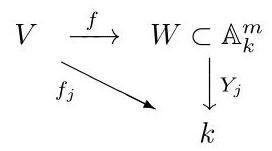
\includegraphics[max width=0.2\textwidth]{images/bo_d3lj80c601uc738kffi0_71_637_1756_272_151_0.jpg}
\end{center}
\hspace*{3em} 

\begin{proof}
这很明显：若 \(f\) 由 \({F}_{1},\ldots ,{F}_{m}\) 给出，则复合映射即为 \(P \mapsto  {F}_{j}(P)\)，它是一个多项式函数.反之，若对每个 \(j\) 都有 \({f}_{j} \in  k[V]\)，则我们可以选取任意 \({F}_{j} \in  k[X_1, \ldots, X_n]\) 使得 \({f}_{j} = {F}_{j} \pmod{I(V)}\)，从而得到 \(f\) 作为由 \((F_1, \ldots, F_m)\) 给出的多项式映射的描述.根据此命题，映射 \(f\) 可写作 \(f = (f_1, \ldots, f_m)\).
\end{proof}

多项式映射的复合以一种自然的方式定义：设 \(V \subset  {\mathbb{A}}^{n}, W \subset  {\mathbb{A}}^{m}\) 和 \(U \subset  {\mathbb{A}}^{\ell}\) 为代数集，且 \(f : V \rightarrow  W, g : W \rightarrow  U\) 为多项式映射，则复合映射 \(g \circ  f : V \rightarrow  U\) 仍然是多项式映射.若 \(f\) 由 \({F}_{1},\ldots ,{F}_{m} \in  k[X_1, \ldots, X_n]\) 给出，且 \(g\) 由 \({G}_{1},\ldots ,{G}_{\ell } \in k[Y_1, \ldots, Y_m]\) 给出，则 \(g \circ  f\) 由以下多项式给出：
\[
{G}_{1}(F_1, \ldots, F_m), \ldots, {G}_{\ell}(F_1, \ldots, F_m) \in  k[X_1, \ldots, X_n].
\]

\begin{definition}[同构]
代数集之间的多项式映射 \(f : V \rightarrow  W\) 称为\textbf{同构}（isomorphism），如果存在一个多项式映射 \(g : W \rightarrow  V\) 使得 \(f \circ  g = \mathrm{id}_W\) 且 \(g \circ  f = \mathrm{id}_V\).
\end{definition}

我们已经见过几个多项式映射的例子：
\begin{itemize}
    \item (2.1)中由 \(t \mapsto  (t^2, t^3)\) 或 \((t^2 - 1, t^3 - t)\) 给出的参数化 \({\mathbb{R}}^{1} \rightarrow  C \subset {\mathbb{R}}^{2}\).
    \item (3.11, b)中由 \(t \mapsto  (t^3, t^4, t^5)\) 定义的映射 \(k \rightarrow  C \subset  {\mathbb{A}}_{k}^{3}\).
    \item 在讨论诺特正规化时，我们有一个代数集 \(V \subset  {\mathbb{A}}_{k}^{n}\)，并考虑了由“相当一般”的线性形式 \({Y}_{1},\ldots ,{Y}_{m}\) 定义的射影 \(p : V \rightarrow  {\mathbb{A}}_{k}^{m}\).由于 \({Y}_{i}\) 是 \({\mathbb{A}}_{k}^{n}\) 上坐标 \({X}_{j}\) 的线性组合，这个射影是一个多项式映射.
\end{itemize}

另一方面，(1.1)中圆的参数化是由有理函数给出的（分母中有一项 \({\lambda }^{2} + 1\)），因此不是多项式映射.同样，从奇异三次曲线 \(C \subset  {\mathbb{R}}^{2}\) 到 \({\mathbb{R}}^{1}\) 的逆映射 \((X,Y) \mapsto  t = Y/X\) 也不是多项式映射.

\section{多项式映射与 \(k[V]\)}

\begin{theorem}
设 \(V \subset  {\mathbb{A}}_{k}^{n}\) 和 \(W \subset  {\mathbb{A}}_{k}^{m}\) 为代数集.
\begin{enumerate}
    \item[\upshape (1)] 一个多项式映射 \(f : V \rightarrow  W\) 诱导一个 \(k\)-代数同态 \({f}^{ * } : k[W] \rightarrow  k[V]\)，该同态由函数复合定义：若 \(g \in  k[W]\) 是一个多项式函数，则 \({f}^{ * }(g) = g \circ  f\) 也是一个多项式函数.映射 \(g \mapsto  g \circ  f\) 定义了一个从 \(k[W]\) 到 \(k[V]\) 的 \(k\)-代数同态.（注意映射方向是反的.）

    \item[\upshape (2)] 反之，任何一个 \(k\)-代数同态 \(\Phi  : k[W] \rightarrow  k[V]\) 都可由一个唯一确定的多项式映射 \(f : V \rightarrow  W\) 诱导，使得 \(\Phi  = {f}^{ * }\).
\end{enumerate}
因此，上述两点表明，通过 \(f \mapsto  {f}^{ * }\) 建立的映射
\[
\left\{ \begin{array}{c} \text{多项式映射} \\ f : V \rightarrow  W \end{array} \right\} \longleftrightarrow \left\{ \begin{array}{c} k\text{-代数同态} \\ \Phi  : k[W] \rightarrow  k[V] \end{array} \right\}
\]
是一个双射.
\begin{enumerate}
    \item[\upshape (3)] 若 \(f : V \rightarrow  W\) 和 \(g : W \rightarrow  U\) 是多项式映射，则复合映射的同态满足 \({\left( g \circ  f\right) }^{ * } = {f}^{ * } \circ  {g}^{ * } : k[U] \rightarrow  k[V]\).
\end{enumerate}
\end{theorem}

\begin{proof}
(1) 根据(4.3)的讨论，\({f}^{ * }(g)\) 是一个从 \(V\) 到 \(k\) 的多项式函数，因此 \({f}^{ * }(g) \in  k[V]\).显然，对所有常数 \(a \in  k\)，\({f}^{ * }(a) = a\).\({f}^{ * }\) 是一个环同态，这是因为 \(k[W]\) 和 \(k[V]\) 都是函数环，其环结构是逐点定义的.例如，对 \({g}_{1},{g}_{2} \in  k[W]\)，和 \({g}_{1} + {g}_{2}\) 定义为对所有 \(P \in  W\)，\((g_1 + g_2)(P) = g_1(P) + g_2(P)\).因此，\({f}^{ * }(g_1 + g_2)(Q) = (g_1 + g_2)(f(Q)) = g_1(f(Q)) + g_2(f(Q)) = {f}^{ * }g_1(Q) + {f}^{ * }g_2(Q)\).

(3) 这仅仅是函数复合满足结合律的体现.

(2) 这部分的表述需要一些技巧，但内容依然是直接的.对 \(i = 1,\ldots ,m\)，令 \({y}_{i} \in  k[W]\) 为 \(W\) 上的第 \(i\) 个坐标函数，因此
\[
k[W] = k[y_1, \ldots, y_m] = k[Y_1, \ldots, Y_m]/I(W).
\]
给定一个 \(k\)-代数同态 \(\Phi  : k[W] \rightarrow  k[V]\)，我们可以定义 \({f}_{i} = \Phi(y_i) \in  k[V]\).

现在考虑由 \(f(P) = (f_1(P), \ldots, f_m(P))\) 定义的映射 \(f : V \rightarrow  {\mathbb{A}}_{k}^{m}\).这是一个多项式映射，因为每个 \({f}_{i}\) 都是 \(k[V]\) 中的元素.我们断言 \(f\) 将 \(V\) 映入 \(W\)，即 \(f(V) \subset  W\).
确实，假设 \(G \in  I(W) \subset  k[Y_1, \ldots, Y_m]\)；那么在环 \(k[W]\) 中，我们有
\[
G(y_1, \ldots, y_m) = 0.
\]
将同态 \(\Phi\) 应用于此等式，得到 \( \Phi(G(y_1, \ldots, y_m)) = 0 \in  k[V]\).由于 \(\Phi\) 是一个 \(k\)-代数同态，
\[
0 = \Phi(G(y_1, \ldots, y_m)) = G(\Phi(y_1), \ldots, \Phi(y_m)) = G(f_1, \ldots, f_m).
\]
这里的 \({f}_{i}\) 是定义在 \(V\) 上的函数，而 \(G(f_1, \ldots, f_m) \in  k[V]\) 是函数 \(P \mapsto  G(f_1(P), \ldots, f_m(P))\).这表明，对任意 \(P \in  V\) 和任意 \(G \in  I(W)\)，点 \(f(P)\) 的坐标 \((f_1(P), \ldots, f_m(P))\) 满足 \(G(f_1(P), \ldots, f_m(P)) = 0\).由于 \(W\) 是由 \(I(W)\) 中多项式的零点定义的，这意味着 \(f(P) \in  W\).

因此，\(f\) 是一个多项式映射 \(f : V \rightarrow  W\).要验证两个 \(k\)-代数同态 \({f}^{ * }\) 和 \(\Phi\) 是否一致，只需检查它们在生成元上的取值.根据 \(f\) 的构造，\({f}^{ * }(y_i) = y_i \circ f = f_i = \Phi(y_i)\)，所以它们是一致的.类似的论证也表明，映射 \(f\) 由条件 \({f}^{ * }(y_i) = \Phi(y_i)\) 唯一确定.
\end{proof}

\begin{corollary}
一个多项式映射 \(f : V \rightarrow  W\) 是同构，当且仅当它诱导的同态 \({f}^{ * } : k[W] \rightarrow  k[V]\) 是一个同构.
\end{corollary}

\paragraph{例子} 在无限域 \(k\) 上，多项式映射
\[
\varphi  : {\mathbb{A}}_{k}^{1} \rightarrow  C : (Y^2 = X^3) \subset  {\mathbb{A}}_{k}^{2} \quad \text{由 } T \mapsto  (T^2, T^3) \text{ 给出}
\]
不是一个同构.因为在这种情况下，同态
\[
{\varphi }^{ * } : k[C] = k[X,Y]/(Y^2 - X^3) \rightarrow  k[T]
\]
由 \(X \mapsto  T^2, Y \mapsto  T^3\) 给出.\({\varphi }^{ * }\) 的像是 \(k[T^2, T^3]\)，这是一个严格小于 \(k[T]\) 的子代数（例如，\(T\) 就不在其像中）.

注意，\(\varphi\) 是一个双射，因此存在一个完美的逆映射 \(\psi  : C \rightarrow  {\mathbb{A}}_{k}^{1}\)，当 \((X,Y) = (0,0)\) 时取值为0，否则为 \(Y/X\).那么为什么 \(\varphi\) 不是同构呢？关键在于 \(C\) 上的多项式函数比 \({\mathbb{A}}^{1}\) 上的要少.直观上讲，\(\varphi\) “压缩”了原点处的切向量.

\section{仿射簇}

设 \(k\) 为一个域.我们希望将\textbf{仿射簇}（affine variety）定义为一个不可约代数子集 \(V \subset  {\mathbb{A}}_{k}^{n}\)，且该定义在同构意义下是明确的.

定理4.4告诉我们，坐标环 \(k[V]\) 是簇 \(V\) 的一个同构不变量.这使我们能够给出一个不那么依赖于嵌入空间 \({\mathbb{A}}_{k}^{n}\) 的簇的定义.这样做的动机比较微妙，如果暂时忽略它，也不会有太大损失.后续对仿射簇的引用将始终采用 \(V \subset {\mathbb{A}}^n\) 的形式.

\begin{definition}
域 \(k\) 上的一个\textbf{仿射簇}是一个集合 \(V\) 以及其上的一个 \(k\)-值函数环 \(k[V]\)，满足：
\begin{enumerate}
    \item \(k[V]\) 是一个有限生成的 \(k\)-代数；
    \item 对于 \(k[V]\) 的某组生成元 \({x}_{1},\ldots ,{x}_{n}\)，映射
    \[
    V \rightarrow  {\mathbb{A}}_{k}^{n} \quad \text{由 } P \mapsto  (x_1(P), \ldots, x_n(P)) \text{ 定义}
    \]
    将 \(V\) 嵌入为一个不可约代数集.
\end{enumerate}
\end{definition}

\section{函数域}

设 \(V\) 为一个仿射簇.其坐标环 \(k[V]\) 是一个整环，其元素是定义在 \(V\) 上的函数.

\begin{definition}
\(V\) 的\textbf{函数域}（function field）\(k(V)\) 是其坐标环 \(k[V]\) 的分式域，即 \(k(V) = \operatorname{Quot}(k[V])\).\(k(V)\) 中的元素 \(f\) 称为 \(V\) 上的\textbf{有理函数}（rational function）.注意，\(f \in  k(V)\) 被定义为一个分式 \(f = g/h\)，其中 \(g,h \in  k[V]\) 且 \(h \neq  0\).
\end{definition}

一个有理函数 \(f\) 先验地并不是在 \(V\) 上处处定义的函数，因为分母 \(h\) 可能有零点.然而，只要 \(h(P) \neq  0\)，\(f\) 在点 \(P \in  V\) 处就是良定义的，因此它至少是一个“部分定义的函数”.

\begin{definition}
设 \(f \in  k(V)\) 和 \(P \in  V\).如果存在一个表达式 \(f = g/h\)，其中 \(g,h \in  k[V]\) 且 \(h(P) \neq  0\)，则称 \(f\) 在 \(P\) 处是\textbf{正则的}（regular），或称 \(P\) 属于 \(f\) 的\textbf{定义域}（domain of definition）.
\end{definition}

需要注意的一个重要事实是，\(k[V]\) 通常不是唯一分解整环（UFD），因此一个有理函数 \(f \in  k(V)\) 可能有本质上不同的分式表示 \(f = g/h\).记
\[
\operatorname{dom}(f) = \{ P \in  V \mid  f \text{ 在 } P \text{ 处正则} \}
\]
为 \(f\) 的定义域.在点 \(P\) 处正则的所有有理函数的集合构成一个子环：
\[
{\mathcal{O}}_{V,P} = \{ f \in  k(V) \mid  f \text{ 在 } P \text{ 处正则} \} = k[V][\{ h^{-1} \mid  h(P) \neq  0 \}],
\]
它被称为 \(V\) 在 \(P\) 处的\textbf{局部环}（local ring）.

\begin{theorem}
(I) \(\operatorname{dom}(f)\) 在Zariski拓扑下是一个非空开集，因而是稠密的.

假设域 \(k\) 是代数闭的，则
(II)
\[
\operatorname{dom}(f) = V \Leftrightarrow  f \in  k[V]
\]
（即，处处正则的有理函数就是多项式函数）.此外，对任意 \(h \in  k[V]\)，设
\[
{V}_{h} = V \setminus  V(h) = \{ P \in  V \mid  h(P) \neq  0 \};
\]
则
(III)
\[
\operatorname{dom}(f) \supset  {V}_{h} \Leftrightarrow  f \in  k[V][h^{-1}].
\]
\end{theorem}

\begin{proof}
定义 \(f \in  k(V)\) 的分母理想为
\[
{D}_{f} = \{ h \in  k[V] \mid  hf \in  k[V] \} = \{ h \in  k[V] \mid  \exists \text{ 表达式 } f = g/h \text{ 且 } g \in  k[V] \} \cup  \{ 0\}.
\]
从第一个定义可以看出，\({D}_{f}\) 是 \(k[V]\) 的一个理想.根据定义，
\[
V \setminus  \operatorname{dom}(f) = \{ P \in  V \mid  h(P) = 0 \text{ 对所有 } h \in  {D}_{f} \} = V({D}_{f}),
\]
因此 \(V \setminus  \operatorname{dom}(f)\) 是 \(V\) 的一个代数子集.故 \(\operatorname{dom}(f) = V \setminus  V({D}_{f})\) 是一个开集.由于 \(f\) 是有理函数，\(D_f\) 非零，所以 \(V(D_f) \neq V\)，\(\operatorname{dom}(f)\) 非空，因此根据命题4.2是稠密的.

现在利用零点定理(b)，
\[
\operatorname{dom}(f) = V \Leftrightarrow  V({D}_{f}) = \varnothing  \Leftrightarrow  1 \in  {D}_{f} \Leftrightarrow f \in  k[V].
\]
最后，
\[
\operatorname{dom}(f) \supset  {V}_{h} \Leftrightarrow  h \text{ 在 } V({D}_{f}) \text{ 上为零},
\]
再利用零点定理(c)，
\[
\Leftrightarrow  {h}^{n} \in  {D}_{f} \text{ 对某个 } n>0 \text{ 成立} \Leftrightarrow f = g/{h}^{n} \text{ 对某个 } g \in k[V] \text{ 成立} \Leftrightarrow f \in  k[V][h^{-1}].
\]
证毕.
\end{proof}

\section{有理映射}

设 \(V\) 为一个仿射簇.

\begin{definition}
一个\textbf{有理映射}（rational map）\(f : V \dashrightarrow {\mathbb{A}}_{k}^{n}\) 是由一组有理函数 \({f}_{1},\ldots ,{f}_{n} \in k(V)\) 定义的部分映射，即
\[
f(P) = (f_1(P), \ldots, f_n(P)) \quad \text{对所有 } P \in  \bigcap \operatorname{dom}(f_i).
\]
\end{definition}
根据定义，\(f\) 的定义域是 \(\operatorname{dom}(f) = \bigcap \operatorname{dom}(f_i)\).我们称 \(f\) 在点 \(P \in  V\) 处是正则的，当且仅当 \(P \in  \operatorname{dom}(f)\).
两个仿射簇 \(V \subset  {\mathbb{A}}^{n}\) 和 \(W \subset  {\mathbb{A}}^{m}\) 之间的有理映射 \(f : V \dashrightarrow W\) 是一个有理映射 \(f : V \dashrightarrow {\mathbb{A}}^{m}\)，且满足 \(f(\operatorname{dom}(f)) \subset  W\).

\section{有理映射的复合}

有理映射 \(f : V \dashrightarrow W\) 和 \(g : W \dashrightarrow U\) 的复合 \(g \circ  f\) 可能没有定义.这是因为有理映射本质上不是一个处处定义的映射：从几何上看，复合映射定义在 \(\operatorname{dom}(f) \cap  f^{-1}(\operatorname{dom}(g))\) 上，但这个集合可能为空.

从代数角度看，同样的问题也存在.假设 \(f\) 由 \({f}_{1},\ldots ,{f}_{m} \in k(V)\) 给出，它定义了 \(f : V \dashrightarrow W \subset  {\mathbb{A}}^{m}\).这诱导了一个 \(k\)-代数同态 \({f}^{ * } : k[W] \rightarrow  k(V)\).然而，如果 \(h \in  k[W]\) 属于 \({f}^{ * }\) 的核，那么我们就无法为 \({f}^{ * }(g/h)\) 赋予任何意义，因此 \({f}^{ * }\) 无法扩展为一个域同态 \(k(W) \rightarrow  k(V)\).

\begin{definition}
一个有理映射 \(f : V \dashrightarrow W\) 是\textbf{占优的}（dominant），如果其像 \(f(\operatorname{dom}(f))\) 在 \(W\) 的Zariski拓扑下是稠密的.
\end{definition}

从几何上讲，这意味着对于任意有理映射 \(g : W \dashrightarrow U\)，集合 \(f^{-1}(\operatorname{dom}(g))\) 是 \(V\) 的一个稠密开集，因此 \(g \circ  f\) 也在 \(V\) 的一个稠密开集上有定义，从而定义了一个从 \(V\) 到 \(U\) 的有理映射.
从代数角度看，
\[
f \text{ 是占优的 } \Leftrightarrow  {f}^{ * } : k[W] \rightarrow  k(V) \text{ 是单射.}
\]
因为对于 \(g \in  k[W]\)，\(g \in  \ker({f}^{ * }) \Leftrightarrow  f(\operatorname{dom}(f)) \subset  V(g)\)，即当且仅当 \(f(\operatorname{dom}(f))\) 包含在 \(W\) 的一个严格代数子集内时，\({f}^{ * }\) 才不是单射.

显然，若 \(f\) 是占优的，则有理映射 \(f\) 和 \(g\) 的复合 \(g \circ  f\) 是有定义的.

\begin{theorem}
(I) 一个占优的有理映射 \(f : V \dashrightarrow W\) 定义了一个域同态 \({f}^{ * } : k(W) \rightarrow  k(V)\).

(II) 反之，一个 \(k\)-同态 \(\Phi  : k(W) \rightarrow  k(V)\) 来源于一个唯一确定的占优有理映射 \(f : V \dashrightarrow W\).

(III) 若 \(f\) 和 \(g\) 均为占优映射，则 \({\left( g \circ  f\right) }^{ * } = {f}^{ * } \circ  {g}^{ * }\).
\end{theorem}
\begin{proof}
证明只需对定理4.4的证明做少量修改.
\end{proof}

\section{从仿射簇的开子集出发的态射}

设 \(V,W\) 为仿射簇，\(U \subset  V\) 为其开子集.

\begin{definition}
一个\textbf{态射}（morphism）\(f : U \rightarrow  W\) 是一个有理映射 \(f : V \dashrightarrow W\)，满足 \(U \subset  \operatorname{dom}(f)\).
\end{definition}

若 \({U}_{1} \subset  V\) 和 \({U}_{2} \subset  W\) 均为开集，则态射 \(f : {U}_{1} \rightarrow  {U}_{2}\) 是一个满足 \(f(U_1) \subset  U_2\) 的态射 \(f : {U}_{1} \rightarrow  W\).同构是一个具有双边逆态射的态射.

注意，若 \(V,W\) 为仿射簇，则根据定理4.8(II)，
\[
\{ \text{态射 } f : V \rightarrow  W \} = \{ \text{多项式映射 } f : V \rightarrow  W \};
\]
等式左侧由满足正则性条件的有理对象组成，而右侧则以更直接的多项式形式表达.

\paragraph{例子} (2.1)中尖点三次曲线 \({\mathbb{A}}^{1} \rightarrow  C : (Y^2 = X^3)\) 的参数化诱导了一个同构 \({\mathbb{A}}^{1} \setminus  \{ 0\}  \cong  C \setminus  \{ (0,0) \}\)；详见例4.5.

\section{标准开子集}

设 \(V\) 为一个仿射簇.对于 \(f \in  k[V]\)，记 \({V}_{f}\) 为开集 \({V}_{f} = V \setminus  V(f) = \{ P \in  V \mid f(P) \neq  0\}\).这些 \({V}_{f}\) 称为 \(V\) 的\textbf{标准开集}（principal open sets）.

\begin{proposition}
标准开集 \({V}_{f}\) 同构于一个仿射簇，且其坐标环为
\[
k[{V}_{f}] = k[V][f^{-1}].
\]
\end{proposition}

\begin{proof}
思路是考虑函数 \(1/f\) 的图像，这个技巧在零点定理(3.10)的证明中也曾使用.

\begin{center}
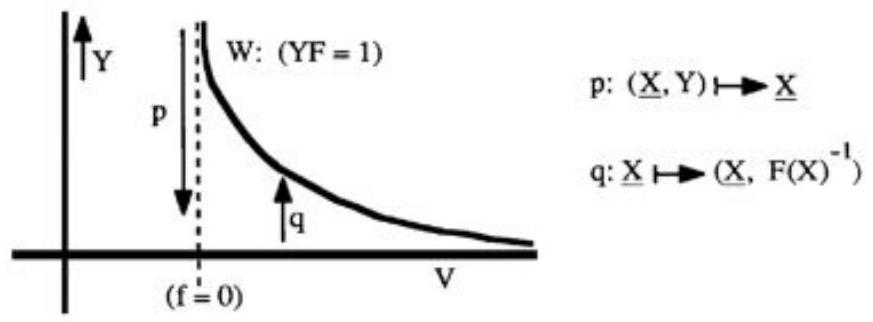
\includegraphics[max width=0.6\textwidth]{images/bo_d3lj80c601uc738kffi0_77_525_1233_873_322_0.jpg}
\end{center}
\hspace*{3em} 

图4.1: \(1/f\) 的图像

设 \(J = I(V) \subset  k[X_1, \ldots, X_n]\)，并选择 \(F \in  k[X_1, \ldots, X_n]\) 使得 \(f = F \pmod{I(V)}\).现在定义理想 \(I = (J, YF - 1) \subset  k[X_1, \ldots, X_n, Y]\)，并令
\[
W = V(I) \subset  {\mathbb{A}}^{n + 1}.
\]
容易验证，图中所示的投影映射 \(\pi: W \to V_f\) 和它的逆映射 \(\sigma: V_f \to W, P \mapsto (P, 1/f(P))\) 都是态射，从而建立了 \(W\) 与 \({V}_{f}\) 之间的同构.关于坐标环的结论包含在定理4.8(III)中.
\end{proof}

标准开集 \({V}_{f}\) 很重要，因为它们构成了 \(V\) 的Zariski拓扑的一个基：每个开集 \(U \subset  V\) 都是标准开集的并（因为每个闭集都形如 \(V(I) = \bigcap_{f \in I} V(f)\)）.因此，上述命题的意义在于，每个开集 \(U \subset  V\) 都是由仿射簇形式的开集 \({V}_{f}\) 拼接而成的.

\section{例子：三次曲线上的群律}

在第2章中，我们讨论了平面非奇异射影三次曲线 \(C \subset  {\mathbb{P}}^{2}\) 上的加法法则 \((A,B) \mapsto  A + B\).设 \({C}_{0} : (y^2 = x^3 + ax + b)\) 为一条非奇异仿射三次曲线.

\begin{center}
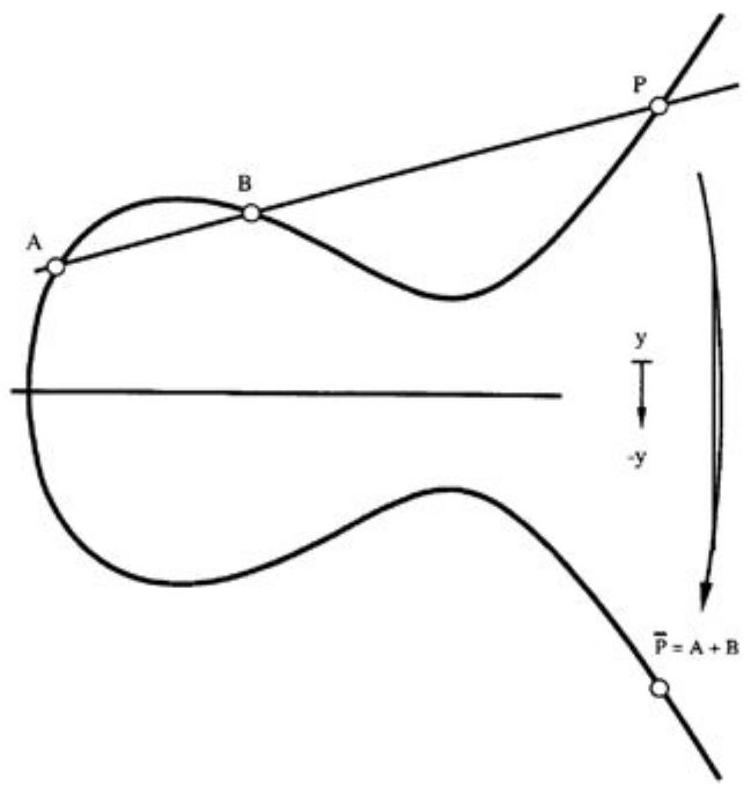
\includegraphics[max width=0.5\textwidth]{images/bo_d3lj80c601uc738kffi0_78_468_683_748_789_0.jpg}
\end{center}
\hspace*{3em} 

图4.2: 三次曲线上的群律作为态射

我们在此展示加法法则定义了一个有理映射 \(\varphi  : {C}_{0} \times  {C}_{0} \dashrightarrow {C}_{0}\)，且 \(\varphi\) 在其定义域内是一个态射.虽然我们不展开细节，但该论证可用于通过“连续性”给出群法则结合律的另一种证明，该证明适用于任意域.

不难看出（参见练习2.7），若 \(A = (x,y), B = (x',y')\) 且 \(x \neq  x'\)，则设 \(u = (y - y')/(x - x')\)，第三个交点为 \(P = (x'',y'')\)，其中
\[
x'' = f(x,y,x',y') = u^2 - (x + x'),
\]
\[
y'' = g(x,y,x',y') = u^3 + xu + y'.
\]
由于 \(x''\) 和 \(y''\) 是坐标 \((x,y), (x',y')\) 的有理函数，这表明 \(\varphi  : {C}_{0} \times {C}_{0} \dashrightarrow {C}_{0}\) 是一个有理映射.根据给定的公式，\(\varphi\) 在 \(x \neq  x'\) 处是一个态射，因为此时 \(u\) 的分母非零.

现在考虑 \(x = x'\) 的情况.如果 \(y = -y'\)，那么 \(x''\) 和 \(y''\) 应该是无穷大，这对应于直线 \(AB\) 在无穷远点 \(O\) 与射影曲线 \(C\) 相交.然而，如果 \(y = y' \neq  0\)（即 \(A=B\) 且不是2-挠点），则点 \(P = (x'',y'')\) 应该是良定义的.我们断言 \(f,g\) 在此类点上是正则的.为此，注意到
\[
y^2 = x^3 + ax + b \quad \text{且} \quad y'^2 = x'^3 + ax' + b,
\]
得到
\[
y^2 - y'^2 = x^3 - x'^3 + a(x - x').
\]
因此，作为 \({C}_{0} \times  {C}_{0}\) 上的有理函数，我们有等式
\[
u = \frac{y - y'}{x - x'} = \frac{x^2 + xx' + x'^2 + a}{y + y'}.
\]
观察第二个表达式的分母，可知只要 \(y \neq -y'\)，\(u\)（因此 \(f\) 和 \(g\)）就是正则的.

计算的结论是：加法律 \(\varphi  : {C}_{0} \times  {C}_{0} \dashrightarrow {C}_{0}\) 在点 \((A,B) \in  {C}_{0} \times  {C}_{0}\) 处是态射，当且仅当 \(A + B \neq  O\).

\section{第四章习题}

4.1 检验从本章开始到(4.8, I)的陈述对任意域 \(k\) 均成立.特别地，探究它们对有限域的含义.如果 \(k\) 不是代数闭的，请给出(4.8, II)的一个反例.

4.2 设 \(\varphi : {\mathbb{A}}^{1} \rightarrow  {\mathbb{A}}^{3}\) 是由 \(X \mapsto  (X, X^2, X^3)\) 给出的多项式映射.证明 \(\varphi\) 的像是代数子集 \(C \subset  {\mathbb{A}}^{3}\)，且 \(\varphi : {\mathbb{A}}^{1} \rightarrow  C\) 是一个同构.尝试推广此结论.

4.3 设 \({\varphi }_{n} : {\mathbb{A}}^{1} \rightarrow  {\mathbb{A}}^{2}\) 是由 \(X \mapsto  (X^2, X^n)\) 给出的多项式映射.证明：如果 \(n\) 是偶数，\({\varphi }_{n}\) 的像同构于 \({\mathbb{A}}^{1}\)，且 \({\varphi }_{n}\) 在原点之外是二对一的.如果 \(n\) 是奇数，证明 \({\varphi }_{n}\) 是双射，并给出一个有理逆映射.

4.4 证明两个仿射簇之间的态射 \(\varphi : X \rightarrow  Y\) 是 \(X\) 与其像 \(\varphi(X) \subset  Y\) 之间的同构，当且仅当诱导的同态 \(\Phi : k[Y] \rightarrow  k[X]\) 是满射.

4.5 设 \(C : \left( {{Y}^{2} = {X}^{3}}\right)  \subset  {\mathbb{A}}^{2}\) ；则

(a) 由 \(\left( {{T}^{2},{T}^{3}}\right)\) 给出的参数化 \(f : {\mathbb{A}}^{1} \rightarrow  C\) 是多项式映射；

(b) \(f\) 具有由 \(\left( {X,Y}\right)  \mapsto  Y/X\) 定义的有理逆映射 \(g : C \rightarrow  {\mathbb{A}}^{1}\) ；

(c) \(\operatorname{dom}g = C \setminus  \{ \left( {0,0}\right) \}\) ;

(d) \(f\) 和 \(g\) 给出逆同构 \({\mathbb{A}}^{1} \setminus  \{ 0\}  \cong  C \setminus  \{ \left( {0,0}\right) \}\) .

4.6 (i) 证明 \(g \circ  f\) 的定义域可能严格大于 \(\operatorname{dom}f \cap  {f}^{-1}\left( {\operatorname{dom}g}\right)\) .[提示:如果 \(g\) 和 \(f\) 是逆有理映射，这种情况可能发生；尝试Ex. 4.5中的 \(f\) 和 \(g\) .]

(ii) 多元微积分课程中常包含如函数 \(f\left( {x,y}\right)  = {xy}/\left( {{x}^{2} + {y}^{2}}\right)\) 的例子.解释为何当限制在通过(0,0)的任意光滑曲线时， \(f\) 是 \({C}^{\infty }\) ，但作为二维变量的函数却不连续.

4.7 设 \(C : \left( {{Y}^{2} = {X}^{3} + {X}^{2}}\right)  \subset  {\mathbb{A}}^{2}\) ；由 \(\left( {{T}^{2} - }\right.\)  \(1,{T}^{3} - T)\) 给出的熟悉参数化 \(\varphi  : {\mathbb{A}}^{1} \rightarrow  C\) 是多项式映射，但不是同构(为什么？).判断其限制 \({\varphi }^{\prime } : {\mathbb{A}}^{1} \setminus  \{ 1\}  \rightarrow  C\) 是否为同构:

\begin{center}

\includegraphics[max width=0.2\textwidth]{images/bo_d3lj80c601uc738kffi0_80_716_422_258_177_0.jpg}
\end{center}
\hspace*{3em} 

图4.3:带缺口的结点曲线

4.8 设 \(C : \left( {{Y}^{3} = {X}^{4} + {X}^{3}}\right)  \subset  {\mathbb{A}}^{2}\) ；证明 \(\left( {X,Y}\right)  \mapsto  X/Y\) 定义了有理映射 \(\psi  : C \rightarrow  {\mathbb{A}}^{1}\) ，其逆映射是多项式映射 \(\varphi  : {\mathbb{A}}^{1} \rightarrow  C\) ，参数化了 \(C\) .证明 \(\varphi\) 限制为同构

\[
{\mathbb{A}}^{1} \setminus  \{ 3\text{ pts. }\}  \cong  C \setminus  \{ \left( {0,0}\right) \} .
\]

4.9 设 \(V : \left( {{XT} = {YZ}}\right)  \subset  {\mathbb{A}}^{4}\) ；解释为何 \(k\left\lbrack  V\right\rbrack\) 不是唯一分解整环(UFD).(理解不难，但给出严格证明较难.) 若 \(f = X/Y \in  k\left( V\right)\) ，求 \(\operatorname{dom}f\) ，并证明其严格包含于闭子集 \(\left( {Y = 0}\right)  \subset  V\) .

4.10 设 \(f : {\mathbb{A}}^{1} \rightarrow  {\mathbb{A}}^{2}\) 由 \(X \mapsto  \left( {X,0}\right)\) 给出，且设 \(g : {\mathbb{A}}^{2} \rightarrow  {\mathbb{A}}^{1}\) 是由 \(\left( {X,Y}\right)  \mapsto  X/Y\) 给出的有理映射；证明复合映射 \(g \circ  f\) 在任何点都未定义.确定函数域 \(k\left( {\mathbb{A}}^{1}\right)\) 中 \({g}^{ * }\) 定义的最大子集.

4.11 定义并研究两个代数集的乘积的概念.更具体地，

(i) 若 \(V \subset  {\mathbb{A}}_{k}^{n}\) 和 \(W \subset  {\mathbb{A}}_{k}^{m}\) 是代数集，证明 \(V \times  W \subset  {\mathbb{A}}_{k}^{n + m}\) 也是代数集；

(ii) 举例说明 \(V \times  W\) 上的Zariski拓扑不是 \(V\) 和 \(W\) 上的积拓扑；

(iii) 证明若 \(V,W\) 不可约，则 \(\Rightarrow  V \times  W\) 也不可约；

(iv) 证明若 \(V \cong  {V}^{\prime }\) 和 \(W \cong  {W}^{\prime }\) ，则 \(V \times  W \cong  {V}^{\prime } \times  {W}^{\prime }\) .

4.12 (a) 证明任何在原点(0,0)处不正则的 \(f \in  k\left( {\mathbb{A}}^{2}\right)\) ，在经过(0,0)的曲线上的点处也不正则.

(b) 推断 \({\mathbb{A}}^{2} \setminus  \left( {0,0}\right)\) 不是仿射的.[提示:(a)中，利用 \(k\left( {\mathbb{A}}^{2}\right)  = k\left( {X,Y}\right)\) 是唯一分解整环(UFD) \(k\left\lbrack  {X,Y}\right\rbrack\) 的分式域，以及习题3.13(b)的结果；(b)中，假设 \({\mathbb{A}}^{2} \setminus  \left( {0,0}\right)\) 是仿射的，确定其坐标环；然后利用推论4.5得到矛盾.] 第三部分


\part{应用}

\chapter{射影几何与双有理几何}

本章的第一部分旨在将第三、四章的内容推广到射影簇的情形；这部分内容很大程度上是水到渠成的，仅涉及少数几个关键点.本章的其余部分则关注双有理几何，它源于第四章末尾引入的函数域 \(k(V)\) 的概念；这些内容同样适用于射影或仿射的背景.

\section{为什么需要射影簇？}

三次曲线

\(
C : (Y^2Z = X^3 + aXZ^2 + bZ^3) \subset {\mathbb{P}}^2
\)

是两条仿射曲线的并集：

\(
C_0 : (y^2 = x^3 + ax + b) \subset {\mathbb{A}}^2 \quad (\text{C 在 } Z=1 \text{ 上的部分})
\)

和

\(
C_1 : (z_1 = x_1^3 + ax_1z_1^2 + bz_1^3) \subset {\mathbb{A}}^2 \quad (\text{C 在 } Y=1 \text{ 上的部分}),
\)

它们通过如下的同构关系粘合在一起：

\(
C_0 \setminus \{y=0\} \to C_1 \setminus \{z_1=0\}
\)

由

\(
(x,y) \mapsto (x/y, 1/y).
\)

一个更简单的例子是射影直线 \({\mathbb{P}}^1\)，它具有齐次坐标 \((U, V)\)，是两个仿射直线 \({\mathbb{A}}^1\)（分别带有坐标 \(u_0, v_1\)）的并集，通过如下同构粘合而成：

\(
{\mathbb{A}}^1 \setminus \{u_0=0\} \to {\mathbb{A}}^1 \setminus \{v_1=0\}
\)

由

\(
u_0 \mapsto 1/u_0.
\)

通常的图示如下：

\begin{center}
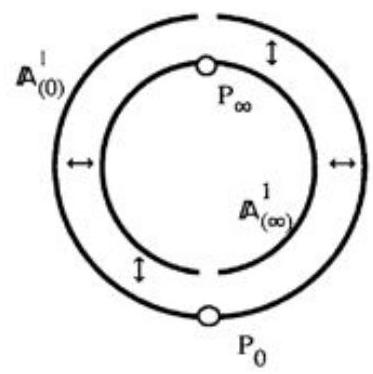
\includegraphics[max width=0.2\textwidth]{images/bo_d3lj80c601uc738kffi0_85_762_364_373_374_0.jpg}
\end{center}
\hspace*{3em} 

图5.1: 由两个 \({\mathbb{A}}^1\) 粘合而成的 \({\mathbb{P}}^1\)

（箭头 \(\leftrightarrow\) 表示粘合过程）.

重要的是要理解，这些簇本身并非仿射簇.事实上，利用即将引入的态射概念，可以证明对于任意 \(n\)，不存在非平凡的态射 \({\mathbb{P}}^1 \to {\mathbb{A}}^n\) 或 \(C \to {\mathbb{A}}^n\)（参见习题5.1和5.12，以及(8.10)中的讨论）.

解决此问题的一种方法是定义一个“抽象簇” \(V\)，将其视为仿射簇的并集 \(V = \bigcup V_i\)，并通过适当的规则进行粘合.这类似于拓扑学中流形的定义，是一个很有吸引力的想法，但会引入更多的技术复杂性.使用射影簇则可以避免这些问题，因为我们是在一个现成的环境空间 \({\mathbb{P}}^n\) 中工作.因此，除了需要对齐次多项式进行一些额外处理外，对射影簇的研究并不比仿射簇困难多少.事实上，尽管在初级阶段可能不明显，但射影簇在很大程度上为研究代数簇提供了一个自然的框架（这一点将在(8.11)中从更高级的视角进行简要讨论）.

\section{分次环与齐次理想}

\begin{definition}
一个多项式 \(f \in k[X_0, \ldots, X_n]\) 称为 \(d\) 次\textbf{齐次多项式}（homogeneous polynomial），如果
\(
f = \sum a_{i_0\ldots i_n}X_0^{i_0}\cdots X_n^{i_n} \text{，其中 } a_{i_0\ldots i_n} \neq 0 \text{ 仅当 } i_0 + \cdots + i_n = d.
\)
\end{definition}
任意多项式 \(f \in k[X_0, \ldots, X_n]\) 都有唯一的表达式 \(f = f_0 + f_1 + \cdots + f_N\)，其中每个 \(f_d\) 都是 \(d\) 次齐次多项式.

\begin{proposition}
若 \(f\) 是一个 \(d\) 次齐次多项式，则对任意 \(\lambda \in k\)，
\(
f(\lambda X_0, \ldots, \lambda X_n) = \lambda^d f(X_0, \ldots, X_n);
\)
若 \(k\) 是无限域，则其逆命题也成立.
\end{proposition}
\begin{proof}
直接验证即可.
\end{proof}

\begin{definition}
一个理想 \(I \subset k[X_0, \ldots, X_n]\) 称为\textbf{齐次理想}（homogeneous ideal），如果对任意 \(f \in I\)，其齐次分解 \(f = f_0 + f_1 + \cdots + f_N\) 中的每个齐次分量 \(f_i\) 都属于 \(I\).
\end{definition}

一个等价的定义是，理想 \(I\) 可由有限个齐次多项式生成.

\section{齐次的 \(V-I\) 对应}

设 \({\mathbb{P}}_k^n\) 为定义在域 \(k\) 上的 \(n\) 维射影空间，其齐次坐标为 \(X_0, \ldots, X_n\).一个多项式 \(f \in k[X_0, \ldots, X_n]\) 并非 \({\mathbb{P}}_k^n\) 上的函数.根据定义，\({\mathbb{P}}_k^n = (k^{n+1} \setminus \{0\}) / \sim\)，其中等价关系 \(\sim\) 定义为 \((X_0, \ldots, X_n) \sim (\lambda X_0, \ldots, \lambda X_n)\)，对任意 \(\lambda \in k \setminus \{0\}\) 成立.因此，\(f\) 实际上是 \(k^{n+1}\) 上的函数.

然而，对于齐次多项式 \(f\)，条件 \(f(P) = 0\) 在 \(P \in {\mathbb{P}}^n\) 上是良定义的.设点 \(P\) 的齐次坐标为 \((X_0 : \cdots : X_n)\)，这意味着 \((X_0, \ldots, X_n)\) 是 \(P\) 在 \(k^{n+1} \setminus \{0\}\) 中所在等价类的一个代表元.由于 \(f(\lambda \mathbf{X}) = \lambda^d f(\mathbf{X})\)，若 \(f(X_0, \ldots, X_n) = 0\)，则 \(f(\lambda X_0, \ldots, \lambda X_n) = 0\) 也成立.因此，条件 \(f(P) = 0\) 与代表元的选择无关.

基于此，我们可以像在仿射情形中一样，定义 \(V\) 和 \(I\) 之间的对应关系：

\(
\{ \text{齐次理想 } J \subset k[X_0, \ldots, X_n] \} \overset{V-I}{\longleftrightarrow} \{ \text{子集 } X \subset {\mathbb{P}}_k^n \}
\)

具体定义如下：

\(
V(J) = \{ P \in {\mathbb{P}}_k^n \mid f(P) = 0 \text{ 对所有齐次 } f \in J \}
\)

以及

\(
I(X) = \{ f \in k[X_0, \ldots, X_n] \mid f(P) = 0 \text{ 对所有 } P \in X \}.
\)
读者可以自行验证 \(I(X)\) 确实是一个齐次理想.

对应关系 \(V\) 和 \(I\) 满足与第三章中引入的仿射对应关系相同的形式性质（例如 \(V(J_1 + J_2) = V(J_1) \cap V(J_2)\)）.形如 \(V(I)\) 的子集称为 \({\mathbb{P}}_k^n\) 的\textbf{代数子集}（algebraic subset）.与仿射情形类似，\({\mathbb{P}}_k^n\) 具有Zariski拓扑，其闭集就是代数子集.

\section{射影零点定理}

与仿射对应关系一样，\(V(I(X)) = X\) 对任意代数集 \(X\) 成立，而 \(I(V(J)) = \operatorname{rad}J\) 则需要零点定理的保证.这里有一个需要注意的细节：平凡理想 \((1) = k[X_0, \ldots, X_n]\) 在 \(k^{n+1}\) 中定义了空集，因此在 \({\mathbb{P}}_k^n\) 中也定义了空集.然而，理想 \((X_0, \ldots, X_n)\) 在 \(k^{n+1}\) 中定义了原点 \(\{0\}\)，这在 \({\mathbb{P}}_k^n\) 中同样对应空集.这个理想 \((X_0, \ldots, X_n)\) 被称为\textbf{无关理想}（irrelevant ideal），它在理论的几个命题中是一个需要特殊处理的例外.

零点定理的齐次版本如下：

\begin{theorem}[射影零点定理]
假设 \(k\) 是一个代数闭域.则
\begin{enumerate}
    \item[\upshape (i)] \(V(J) = \varnothing \Leftrightarrow \operatorname{rad}J \supset (X_0, \ldots, X_n)\)；
    \item[\upshape (ii)] 如果 \(V(J) \neq \varnothing\)，则 \(I(V(J)) = \operatorname{rad}J\).
\end{enumerate}
\end{theorem}

\begin{corollary}
映射 \(I\) 和 \(V\) 确定了如下的逆双射：
\(
\left\{ \begin{array}{c} \text{不含于 } \{X_0=0\} \text{ 的} \\ \text{不可约代数子集 } V \subset {\mathbb{P}}^n \end{array} \right\} \longleftrightarrow \left\{ \begin{array}{c} \text{不可约代数子集} \\ V_0 \subset {\mathbb{A}}_{(0)}^n \end{array} \right\}
\)

以及
\(
\left\{ \begin{array}{c} \text{不包含无关理想的} \\ \text{齐次根理想} \\ J \subset k[x_0, \ldots, x_n] \end{array} \right\} \longleftrightarrow \left\{ \begin{array}{c} \text{代数子集} \\ X \subset {\mathbb{P}}^n \end{array} \right\}
\)

以及
\(
\left\{ \begin{array}{c} \text{不包含无关理想的} \\ \text{齐次素理想} \\ J \subset k[x_0, \ldots, x_n] \end{array} \right\} \longleftrightarrow \left\{ \begin{array}{c} \text{不可约代数子集} \\ X \subset {\mathbb{P}}^n \end{array} \right\}
\)
\end{corollary}

\begin{proof}
令 \(\pi : {\mathbb{A}}^{n+1} \setminus \{0\} \to {\mathbb{P}}^n\) 为定义 \({\mathbb{P}}^n\) 的商映射.对于齐次理想 \(J \subset k[X_0, \ldots, X_n]\)，我们用 \(V^a(J) \subset {\mathbb{A}}^{n+1}\) 表示由 \(J\) 定义的仿射代数集.由于 \(J\) 是齐次的，\(V^a(J)\) 是一个锥，即

\(
(\alpha_0, \ldots, \alpha_n) \in V^a(J) \Leftrightarrow (\lambda\alpha_0, \ldots, \lambda\alpha_n) \in V^a(J) \text{ 对所有 } \lambda \in k.
\)

并且 \(V(J) = (V^a(J) \setminus \{0\}) / \sim\).因此

\(
V(J) = \varnothing \Leftrightarrow V^a(J) \subset \{0\} \Leftrightarrow \operatorname{rad}J \supset (X_0, \ldots, X_n),
\)

最后一步推论使用了仿射零点定理.此外，如果 \(V(J) \neq \varnothing\)，则

\(
f \in I(V(J)) \Leftrightarrow f \in I(V^a(J)) \Leftrightarrow f \in \operatorname{rad}J.
\)

证毕.
\end{proof}
上述出现的仿射子集 \(V^a(J)\) 称为射影代数子集 \(V(J)\) 上的\textbf{仿射锥}（affine cone）.

\section{\(V\) 上的有理函数}

设 \(V \subset {\mathbb{P}}_k^n\) 为一个不可约代数集，其理想为 \(I(V) \subset k[X_0, \ldots, X_n]\).我们无法直接用多项式来定义 \(V\) 上的正则函数：一个元素 \(F \in k[X_0, \ldots, X_n]\) 在 \(V\) 的仿射锥上给出一个函数，但只有当 \(F\) 是0次齐次（即常数）时，该函数才在等价类上保持不变.因此，我们从一开始就只考虑有理函数.

\begin{definition}
\(V\) 上的\textbf{有理函数}（rational function）是一个部分定义的函数 \(f : V \dashrightarrow k\)，由 \(f(P) = g(P)/h(P)\) 给出，其中 \(g, h \in k[X_0, \ldots, X_n]\) 是同次幂的齐次多项式.只要 \(h(P) \neq 0\)，这个商就是良定义的，因为

\(
g(\lambda\mathbf{X})/h(\lambda\mathbf{X}) = \lambda^d g(\mathbf{X})/\lambda^d h(\mathbf{X}) = g(\mathbf{X})/h(\mathbf{X}) \quad \text{对 } 0 \neq \lambda \in k.
\)
\end{definition}

两个分式 \(g/h\) 和 \(g'/h'\) 在 \(V\) 上定义相同的有理函数，当且仅当 \(h'g - g'h \in I(V)\).因此，所有有理函数的集合构成一个域：

\(
k(V) = \left\{ \left. \frac{g}{h} \right| \begin{array}{l} g,h \in k[X_0, \ldots, X_n] \text{ 是同次幂的} \\ \text{齐次多项式，且 } h \notin I(V) \end{array} \right\} / \sim,
\)

其中 \(\sim\) 是等价关系 \(g/h \sim g'/h' \Leftrightarrow h'g - g'h \in I(V)\).这个域 \(k(V)\) 称为 \(V\) 的\textbf{函数域}（function field）.

以下定义与仿射情形完全相同.对于 \(f \in k(V)\) 和 \(P \in V\)，如果存在表达式 \(f = g/h\)，其中 \(g,h\) 是同次幂的齐次多项式且 \(h(P) \neq 0\)，则称 \(f\) 在 \(P\) 处是\textbf{正则的}（regular）.记

\(
\operatorname{dom}(f) = \{ P \in V \mid f \text{ 在 } P \text{ 处正则} \}
\)

和

\(
\mathcal{O}_{V,P} = \{ f \in k(V) \mid f \text{ 在 } P \text{ 处正则} \}
\)

为 \(V\) 在 \(P\) 处的局部环.

显然，\(\operatorname{dom}(f) \subset V\) 是 \(V\) 中的一个稠密Zariski开集（证明同(4.8, I)），且 \(\mathcal{O}_{V,P} \subset k(V)\) 是一个子环.

\section{射影簇的仿射覆盖}

设 \(V \subset {\mathbb{P}}^n\) 为一个不可约代数集.为简便起见，我们假设对任意 \(i\)，\(V\) 不包含在超平面 \(\{X_i = 0\}\) 中.我们知道 \({\mathbb{P}}^n\) 被 \(n+1\) 个标准仿射开集 \({\mathbb{A}}_{(i)}^n\) 覆盖，这些开集具有仿射（非齐次）坐标

\(
X_0^{(i)}, \ldots, X_{i-1}^{(i)}, X_{i+1}^{(i)}, \ldots, X_n^{(i)}, \quad \text{其中 } X_j^{(i)} = X_j/X_i.
\)

记 \(V_{(i)} = V \cap {\mathbb{A}}_{(i)}^n\).那么 \(V_{(i)} \subset {\mathbb{A}}_{(i)}^n\) 是一个仿射代数集，因为

\(
P = (1, x_1^{(0)}, \ldots, x_n^{(0)}) \in V_{(0)} \Leftrightarrow f(1, x_1^{(0)}, \ldots, x_n^{(0)}) = 0 \text{ 对所有齐次 } f \in I(V),
\)

这是一个关于 \(P\) 的坐标 \((x_1^{(0)}, \ldots, x_n^{(0)})\) 的多项式方程组.为清晰起见，我们在论证中取 \(i=0\)，并将在方便时继续这样做.这些 \(V_{(i)}\) 称为 \(V\) 的\textbf{标准仿射片}（standard affine charts）.

\begin{proposition}
\begin{enumerate}
    \item[\upshape (i)] 对应关系 \(V \mapsto V_{(0)} = V \cap {\mathbb{A}}_{(0)}^n\) 给出了一个双射：
    \[
    \left\{ \begin{array}{c} \text{不含于 } \{X_0=0\} \text{ 的} \\ \text{不可约代数子集 } V \subset {\mathbb{P}}^n \end{array} \right\} \longleftrightarrow \left\{ \begin{array}{c} \text{不可约代数子集} \\ V_0 \subset {\mathbb{A}}_{(0)}^n \end{array} \right\};
    \]
    其逆对应关系通过在Zariski拓扑中取闭包给出.

    \item[\upshape (ii)] 记 \(V \subset {\mathbb{P}}^n\) 的齐次理想为 \(I^h(V) \subset k[X_0, \ldots, X_n]\)，\(V_{(0)} \subset {\mathbb{A}}_{(0)}^n\) 的非齐次理想为 \(I^a(V_{(0)}) \subset k[X_1, \ldots, X_n]\).则它们之间的关系如下：
    \[
    I^a = \{ f(1, X_1, \ldots, X_n) \mid f \in I^h(V) \},
    \]
    以及
    \[
    I^h(V)_d = \left\{ X_0^d f\left(\frac{X_1}{X_0}, \ldots, \frac{X_n}{X_0}\right) \mid f \in I^a(V_{(0)}), \deg f \le d \right\},
    \]
    其中下标 \(d\) 表示 \(d\) 次齐次部分.

    \item[\upshape (iii)] 函数域 \(k(V) \cong k(V_{(0)})\).对于 \(f \in k(V)\)，其作为 \(V_{(0)}\) 上函数的定义域是 \(V_{(0)} \cap \operatorname{dom}(f)\).
\end{enumerate}
\end{proposition}
\begin{proof}
(i) 和 (ii) 的证明是直接的.(iii) 若 \(g,h \in k[X_0, \ldots, X_n]\) 是 \(d\) 次齐次的，且 \(h \notin I(V)\)，则 \(g/h \in k(V)\) 限制在 \(V_{(0)}\) 上是函数
\(
\frac{g(1, X_1/X_0, \ldots, X_n/X_0)}{h(1, X_1/X_0, \ldots, X_n/X_0)};
\)
这定义了一个映射 \(k(V) \to k(V_{(0)})\)，其逆映射也显而易见.
\end{proof}

\section{有理映射与态射}

射影（或仿射）簇之间的有理映射是通过函数域 \(k(V)\) 定义的.若 \(V \subset {\mathbb{P}}^n\) 是一个不可约代数集，则一个\textbf{有理映射} \(V \dashrightarrow {\mathbb{A}}^m\) 是由 \(P \mapsto (f_1(P), \ldots, f_m(P))\) 给出的部分定义的映射，其中 \(f_1, \ldots, f_m \in k(V)\).一个有理映射 \(V \dashrightarrow {\mathbb{P}}^m\) 则由 \(P \mapsto (f_0(P) : f_1(P) : \cdots : f_m(P))\) 定义，其中 \(f_0, f_1, \ldots, f_m \in k(V)\).注意，若 \(g \in k(V)\) 是非零元素，则 \((gf_0, gf_1, \ldots, gf_m)\) 定义了相同的有理映射.因此，我们可以通过乘以一个合适的公分母，将有理映射表示为齐次多项式的比值.

\begin{definition}
一个有理映射 \(f : V \dashrightarrow {\mathbb{P}}^m\) 在点 \(P \in V\) 处是\textbf{正则的}（regular），如果存在一个表达式 \(f = (f_0 : f_1 : \cdots : f_m)\) 使得
\begin{enumerate}
    \item[\upshape (i)] 每个 \(f_i\) 在 \(P\) 处都是正则的；
    \item[\upshape (ii)] 至少有一个 \(f_i(P) \neq 0\).
\end{enumerate}
\end{definition}
第二个条件保证了 \(f_i\) 之间的比值在 \(P\) 处有定义.如果 \(f\) 在 \(P\) 处正则，那么对于 \(P\) 的某个开邻域 \(U \subset V\)，映射 \(f: U \to {\mathbb{A}}_{(i)}^m \subset {\mathbb{P}}^m\) 是一个态射.

如果 \(U \subset V\) 是射影簇 \(V\) 的一个开子集，则一个\textbf{态射}（morphism）\(f : U \to W\) 是一个有理映射 \(f : V \dashrightarrow W\)，满足 \(\operatorname{dom}(f) \supset U\).换言之，态射是在 \(U\) 上处处正则的有理映射.

\section{例子}

\paragraph{有理正规曲线} 这是一个将 \({\mathbb{P}}^1\) 同构地嵌入到 \({\mathbb{P}}^m\) 中的经典例子，推广了(1.7)中圆锥曲线的参数化，在射影几何和代数几何中都非常重要.定义映射

\(
f : {\mathbb{P}}^1 \to {\mathbb{P}}^m \quad \text{由 } (U:V) \mapsto (U^m : U^{m-1}V : \cdots : V^m) \text{ 给出}
\)

（即 \(U,V\) 的所有 \(m\) 次单项式）.

\begin{enumerate}
    \item[\upshape (i)] \(f\) 是一个有理映射，因为它可以表示为 \(((U/V)^m : (U/V)^{m-1} : \cdots : 1)\).

    \item[\upshape (ii)] 根据此表达式，\(f\) 在 \(V \neq 0\) 的点上是态射.若 \(V=0\)，则 \(U \neq 0\)，我们可以使用关于 \(V/U\) 的类似表达式来证明其正则性.因此 \(f\) 是一个从 \({\mathbb{P}}^1\) 到 \({\mathbb{P}}^m\) 的态射.

    \item[\upshape (iii)] \(f\) 的像 \(C\) 是 \({\mathbb{P}}^m\) 中满足如下条件的点集 \((X_0 : X_1) = (X_1 : X_2) = \cdots = (X_{m-1} : X_m)\)：

\(
(X_0 : X_1) = (X_1 : X_2) = \cdots = (X_{m-1} : X_m),
\)

这等价于方程组 \(X_i X_{j+1} = X_{i+1} X_j\).这些方程可以统一写成一个方便的行列式形式：

\(
\operatorname{rank} \begin{pmatrix} X_0 & X_1 & \cdots & X_{m-1} \\ X_1 & X_2 & \cdots & X_m \end{pmatrix} \le 1
\)

（秩条件意为所有 \(2 \times 2\) 子式都为零）.这些是定义代数集 \(C \subset {\mathbb{P}}^m\) 的齐次方程.

    \item[\upshape (iv)] 逆态射 \(g : C \to {\mathbb{P}}^1\) 很容易找到：只需将 \(C\) 中的点映射到公共比值 \((X_0 : X_1)\).
\end{enumerate}

\paragraph{线性射影与二次曲面的参数化} 映射 \(\pi : {\mathbb{P}}^3 \dashrightarrow {\mathbb{P}}^2\) 由 \((X_0, X_1, X_2, X_3) \mapsto (X_1, X_2, X_3)\) 给出，它是一个有理映射，在点 \(P_0 = (1:0:0:0)\) 之外是态射.设 \(Q \subset {\mathbb{P}}^3\) 是一个包含 \(P_0\) 的二次曲面.那么 \({\mathbb{P}}^2\) 中的每个点 \(P\) 对应于 \({\mathbb{P}}^3\) 中通过 \(P_0\) 和 \(P\) 的一条直线 \(L\).一般情况下，\(L\) 会在 \(P_0\) 和另一个点 \(\varphi(P)\) 处与 \(Q\) 相交.例如，若 \(Q\) 的方程为 \(X_0X_3 = X_1X_2\)，则 \(\pi|_Q : Q \dashrightarrow {\mathbb{P}}^2\) 具有逆映射

\(
\varphi : {\mathbb{P}}^2 \dashrightarrow Q \quad \text{由 } (Y_0:Y_1:Y_2) \mapsto (Y_0Y_1/Y_2 : Y_0 : Y_1 : Y_2) \text{ 给出}.
\)

这本质上与(1.1)中圆的参数化思想相同.这是一个有益的练习（见习题5.2），去找出 \(\operatorname{dom}(\pi)\) 和 \(\operatorname{dom}(\varphi)\)，并给出 \(\pi\) 和 \(\varphi\) 奇异点的几何解释.

\section{双有理等价}

\begin{definition}
两个簇 \(V, W\) 是\textbf{双有理等价的}（birationally equivalent），如果存在占优有理映射 \(f : V \dashrightarrow W\) 和 \(g : W \dashrightarrow V\) 使得 \(f \circ g = \mathrm{id}_W\) 和 \(g \circ f = \mathrm{id}_V\).等价地，它们的函数域 \(k(V)\) 和 \(k(W)\) 是 \(k\)-同构的.
\end{definition}

\begin{theorem}
任意簇 \(V\) 都双有理等价于一个超曲面 \(H \subset {\mathbb{P}}^{d+1}\).
\end{theorem}
\begin{proof}
函数域 \(k(V)\) 是 \(k\) 上的有限生成域扩张.根据代数基本定理，存在一个超越基 \(\{x_1, \ldots, x_d\}\)，使得 \(k(V)\) 是 \(k(x_1, \ldots, x_d)\) 的有限扩张.再根据本原元定理，存在一个元素 \(y\) 使得 \(k(V) = k(x_1, \ldots, x_d, y)\).因此，\(y\) 满足一个以 \(x_i\) 为系数的不可约多项式方程 \(F(x_1, \ldots, x_d, y) = 0\).这定义了一个超曲面 \(H \subset {\mathbb{A}}^{d+1}\)，其函数域为 \(k(V)\).通过取其在 \({\mathbb{P}}^{d+1}\) 中的闭包，我们得到所需的超曲面.
\end{proof}

\section{纤维积与像}

\paragraph{纤维积} 设 \(f: X \to Z\) 和 \(g: Y \to Z\) 是态射.它们的\textbf{纤维积}（fibre product）\(X \times_Z Y\) 定义为

\(
X \times_Z Y = \{ (x,y) \in X \times Y \mid f(x) = g(y) \}.
\)

如果所有簇都是仿射的，\(X \subset {\mathbb{A}}^n, Y \subset {\mathbb{A}}^m, Z \subset {\mathbb{A}}^p\)，则 \(X \times_Z Y \subset {\mathbb{A}}^{n+m}\) 是一个代数集，其坐标环为 \(k[X] \otimes_{k[Z]} k[Y]\).

\paragraph{态射的像} 一个令人惊讶的事实是，一个态射的像不一定是代数集.例如，态射 \(f: {\mathbb{A}}^2 \to {\mathbb{A}}^2\) 由 \((x,y) \mapsto (x, xy)\) 给出，其像是 \({\mathbb{A}}^2 \setminus \{x=0, y \neq 0\}\)，这是一个开集，但不是闭集.

\begin{theorem}[Chevalley]
设 \(f: X \to Y\) 是簇之间的态射.则其像 \(f(X)\) 是一个\textbf{可构造集}（constructible set），即可写成有限个局部闭集（开集与闭集的交集）的并.
\end{theorem}

\section{第五章习题}

5.1 证明不存在从 \({\mathbb{P}}^1\) 到 \({\mathbb{A}}^1\) 的非常数态射.

5.2 考虑(5.7, II)中的二次曲面 \(Q: (X_0X_3 = X_1X_2) \subset {\mathbb{P}}^3\).

\begin{enumerate}
    \item[\upshape (a)] 证明从 \(P_0 = (1:0:0:0)\) 出发的射影 \(\pi: Q \dashrightarrow {\mathbb{P}}^2\) 在两条直线 \(L_1 = V(X_1, X_3)\) 和 \(L_2 = V(X_2, X_3)\) 上是未定义的.

    \item[\upshape (b)] 证明 \(\pi\) 将 \(Q\) 上的其他直线映为 \({\mathbb{P}}^2\) 中的点.

    \item[\upshape (c)] 描述逆映射 \(\varphi: {\mathbb{P}}^2 \dashrightarrow Q\) 的定义域.
\end{enumerate}

5.3 设 \(C \subset {\mathbb{P}}^2\) 是一条由 \(F(X,Y,Z)=0\) 定义的不可约曲线.证明 \(C\) 是有理的（即双有理等价于 \({\mathbb{P}}^1\)）当且仅当存在一个有理映射 \({\mathbb{P}}^1 \dashrightarrow C\) 是占优的.

5.4 证明任何两条二次曲线都是双有理等价的.

5.5 \textbf{Cremona变换}.考虑有理映射 \(f: {\mathbb{P}}^2 \dashrightarrow {\mathbb{P}}^2\) 由 \((X:Y:Z) \mapsto (1/X : 1/Y : 1/Z)\) 定义.

\begin{enumerate}
    \item[\upshape (a)] 写出 \(f\) 的多项式表达式.

    \item[\upshape (b)] 找出 \(f\) 的定义域和像.

    \item[\upshape (c)] 证明 \(f\) 是双有理的，并求出其逆.
\end{enumerate}


\chapter{切空间、非奇异性与维数}

本章旨在为代数簇的维数提供一个恰当的定义，并探讨非奇异性的概念.

\section{超曲面的非奇异点}

假设 \(f \in k[X_1, \ldots, X_n]\) 是一个不可约多项式且 \(f \notin k\)，令 \(V = V(f) \subset \mathbb{A}^n\) 为其定义的超曲面.设 \(P = (a_1, \ldots, a_n) \in V\)，\(\ell\) 是经过 \(P\) 的一条直线.由于 \(P \in V\)，显然 \(P\) 是 \(f\) 限制在直线 \(\ell\) 上的函数 \(f|_{\ell}\) 的一个根.

\textbf{问题：} 何时 \(P\) 是 \(f|_{\ell}\) 的重根？

\textbf{答案：} 当且仅当 \(\ell\) 包含于如下定义的仿射线性子空间
\(
T_P V : \left( \sum_{i=1}^n \frac{\partial f}{\partial X_i}(P) \cdot (X_i - a_i) = 0 \right) \subset \mathbb{A}^n,
\)
该空间称为 \(V\) 在 \(P\) 处的\textbf{切空间}（tangent space）.

\begin{center}
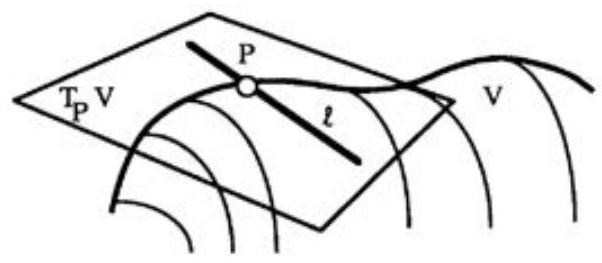
\includegraphics[max width=0.4\textwidth]{images/bo_d3lj80c601uc738kffi0_98_542_1463_602_263_0.jpg}
\end{center}
\hspace*{3em} 

图6.1: 切空间

为证明此点，我们将直线 \(\ell\) 参数化为
\(
\ell: X_i = a_i + b_i T \quad (i=1, \ldots, n)
\)
其中 \(P = (a_1, \ldots, a_n)\)，而 \((b_1, \ldots, b_n)\) 是 \(\ell\) 的方向向量.那么 \(f\) 在 \(\ell\) 上的限制为 \(f|_{\ell} = f(a_1+b_1T, \ldots, a_n+b_nT) = g(T)\)，这是一个关于 \(T\) 的多项式.我们已知 \(T=0\) 是 \(g(T)\) 的一个根.因此，
\(
0 \text{ 是 } g \text{ 的重根} \iff \frac{\mathrm{d}g}{\mathrm{d}T}(0) = 0.
\)
根据链式法则，
\(
\frac{\mathrm{d}g}{\mathrm{d}T}(0) = \sum_{i=1}^n b_i \frac{\partial f}{\partial X_i}(P) = 0.
\)
这个条件等价于直线 \(\ell\) 上的所有点都满足切空间方程，即 \(\ell \subset T_P V\).

\begin{definition}
设 \(V = V(f) \subset \mathbb{A}^n\) 为超曲面，\(P \in V\).若存在某个 \(i\) 使得 \(\frac{\partial f}{\partial X_i}(P) \neq 0\)，则称 \(P\) 是 \(V\) 的\textbf{非奇异点}（non-singular point）；否则，称 \(P\) 是\textbf{奇异点}（singular point），或称 \(V\) 的奇点.
\end{definition}

显然，若 \(P\) 非奇异，则 \(T_P V\) 是 \(\mathbb{A}^n\) 的一个 \(n-1\) 维仿射子空间；若 \(P\) 奇异，则 \(T_P V = \mathbb{A}^n\).

\section{注记}

(a) 上述出现的导数 \(\frac{\partial f}{\partial X_i}(P)\) 是形式上的代数运算（即 \(\frac{\partial}{\partial X_i}\) 将 \(X_i^n\) 映为 \(nX_i^{n-1}\)），不涉及微积分中的极限概念.

(b) 假设 \(k = \mathbb{R}\) 或 \(\mathbb{C}\)，且 \(\frac{\partial f}{\partial X_1}(P) \neq 0\).由 \((X_1, \ldots, X_n) \mapsto (f, X_2, \ldots, X_n)\) 定义的映射 \(p: \mathbb{A}^n \to \mathbb{A}^n\) 在 \(P\) 处的雅可比行列式不为零.根据反函数定理，存在一个邻域 \(P \in U \subset \mathbb{A}^n\)，使得 \(p|_U: U \to p(U) \subset \mathbb{A}^n\) 是邻域 \(U\) 与 \(\mathbb{A}^n\) 的一个开集 \(p(U)\) 之间的微分同胚（在 \(\mathbb{R}^n\) 或 \(\mathbb{C}^n\) 的通常拓扑下）.换言之，\((f, X_2, \ldots, X_n)\) 在 \(P\) 附近构成了 \(\mathbb{A}^n\) 上的一组新的可微坐标系.这意味着 \(V: (f=0)\) 在 \(P\) 的一个邻域与带有坐标 \((X_2, \ldots, X_n)\) 的 \(\mathbb{A}^{n-1}\) 的一个开集微分同胚.因此，在非奇异点附近，\(V\) 是一个以 \((X_2, \ldots, X_n)\) 为局部参数的流形.

\begin{proposition}
非奇异点集 \(V_{\text{nonsing}} = \{ P \in V \mid P \text{ 是非奇异的} \}\) 是 \(V\) 在Zariski拓扑下的一个稠密开集.
\end{proposition}
\begin{proof}
\(V_{\text{nonsing}}\) 的补集是奇异点集 \(V_{\text{sing}}\)，该集合由方程组
\(
f(P) = 0 \quad \text{及} \quad \frac{\partial f}{\partial X_i}(P) = 0 \quad \text{对所有 } i=1, \ldots, n
\)
定义，即 \(V_{\text{sing}} = V(f, \frac{\partial f}{\partial X_1}, \ldots, \frac{\partial f}{\partial X_n}) \subset \mathbb{A}^n\).根据Zariski拓扑的定义，它是一个闭集.

由于 \(V\) 是不可约的，要证明开集 \(V_{\text{nonsing}}\) 是稠密的，我们只需证明它非空即可（根据命题4.2）.采用反证法，假设 \(V_{\text{nonsing}}\) 为空，即 \(V = V(f) = V_{\text{sing}}\).这意味着每个多项式 \(\frac{\partial f}{\partial X_i}\) 都在 \(V\) 上为零.根据零点定理，它们必须在 \(k[X_1, \ldots, X_n]\) 中能被 \(f\) 整除.但作为关于 \(X_i\) 的多项式，\(\frac{\partial f}{\partial X_i}\) 的次数严格小于 \(f\)，所以 \(f\) 整除 \(\frac{\partial f}{\partial X_i}\) 意味着 \(\frac{\partial f}{\partial X_i} = 0\).

若 \(\operatorname{char} k = 0\)，这显然只有在 \(X_i\) 不出现在 \(f\) 中才可能.如果对所有 \(i\) 都如此，则 \(f\) 为常数，与假设矛盾.
若 \(\operatorname{char} k = p > 0\)，\(\frac{\partial f}{\partial X_i} = 0\) 意味着 \(f\) 是 \(X_i\) 的 \(p\)-次多项式，即 \(X_i\) 仅以 \(p\) 的幂次出现在 \(f\) 中.如果对每个 \(i\) 都如此，则 \(f\) 是 \(k[X_1, \ldots, X_n]\) 中的一个 \(p\)-次幂（参见(3.16)），这与 \(f\) 不可约的事实矛盾.证毕.
\end{proof}

\section{一般簇的切空间}

\begin{definition}
设 \(V \subset \mathbb{A}^n\) 为一个子簇，\(P = (a_1, \ldots, a_n) \in V\).对任意 \(f \in k[X_1, \ldots, X_n]\)，记
\(
f_P^{(1)} = \sum_{i=1}^n \frac{\partial f}{\partial X_i}(P) \cdot (X_i - a_i).
\)
这是一个仿射线性多项式，是 \(f\) 在 \(P\) 处的“一阶部分”.\(V\) 在 \(P\) 处的\textbf{切空间}定义为
\(
T_P V = \bigcap_{f \in I(V)} \{ Q \in \mathbb{A}^n \mid f_P^{(1)}(Q) = 0 \} \subset \mathbb{A}^n.
\)
\end{definition}

\begin{proposition}
由 \(P \mapsto \dim T_P V\) 定义的函数 \(V \to \mathbb{N}\) 是一个上半连续函数（在 \(V\) 的Zariski拓扑中）.换言之，对任意整数 \(r\)，子集
\(
S(r) = \{ P \in V \mid \dim T_P V \ge r \} \subset V
\)
是Zariski闭集.
\end{proposition}
\begin{proof}
设 \((f_1, \ldots, f_m)\) 为 \(I(V)\) 的一组生成元.易见，对任意 \(g \in I(V)\)，其线性部分 \(g_P^{(1)}\) 是 \(f_{i,P}^{(1)}\) 的线性组合，因此 \(T_P V\) 的定义简化为
\(
T_P V = \bigcap_{i=1}^m \{ Q \in \mathbb{A}^n \mid f_{i,P}^{(1)}(Q) = 0 \}.
\)
根据初等线性代数，
\(
\dim T_P V = n - \operatorname{rank} J(P), \quad \text{其中 } J(P) = \left( \frac{\partial f_i}{\partial X_j}(P) \right)_{\substack{i=1,\ldots,m \\ j=1,\ldots,n}}.
\)
因此，
\(
P \in S(r) \iff \operatorname{rank} J(P) \le n - r \iff \text{所有 } (n-r+1) \times (n-r+1) \text{ 子式都为零}.
\)
矩阵的每个元素 \(\frac{\partial f_i}{\partial X_j}(P)\) 都是关于 \(P\) 坐标的多项式函数，因此每个子式也是多项式.故 \(S(r) \subset V\) 是一个代数子集，从而是闭集.证毕.
\end{proof}

\begin{definition}
存在一个整数 \(r\) 和一个稠密开子集 \(V_0 \subset V\) 使得
\(
\dim T_P V = r \text{ 对所有 } P \in V_0, \quad \text{且} \quad \dim T_P V \ge r \text{ 对所有 } P \in V.
\)
定义 \(r\) 为 \(V\) 的\textbf{维数}（dimension），记作 \(\dim V = r\).当 \(\dim T_P V = r\) 时，称 \(P \in V\) 为\textbf{非奇异的}；当 \(\dim T_P V > r\) 时，称为\textbf{奇异的}.若一个簇 \(V\) 在其每个点 \(P \in V\) 处都非奇异，则称该簇是\textbf{非奇异的}.
\end{definition}
\begin{proof}
令 \(r = \min \{ \dim T_P V \mid P \in V \}\).则显然
\(
S(r-1) = \varnothing, \quad S(r) = V, \quad \text{且} \quad S(r+1) \subsetneq V;
\)
因此 \(V_0 = S(r) \setminus S(r+1) = \{ P \in V \mid \dim T_P V = r \}\) 是一个非空开集.证毕.
\end{proof}

\section{\(\dim V = \operatorname{tr.deg}_k k(V)\) — 超曲面情形}

由命题6.3可知，若 \(V = V(f) \subset \mathbb{A}^n\) 是由某个非恒定多项式 \(f\) 定义的超曲面，则 \(\dim V = n-1\).另一方面，对于超曲面，有 \(k[V] = k[X_1, \ldots, X_n]/(f)\).因此，假设 \(f\) 确实依赖于 \(X_1\)，则 \(V\) 的函数域为
\(
k(V) = \operatorname{Frac}(k[X_2, \ldots, X_n][X_1]/(f)),
\)
即它是由 \(k\) 添加 \(n-1\) 个代数无关元素，然后再进行一次单代数扩张得到的.

\begin{definition}
若 \(k \subset K\) 是一个域扩张，则 \(K\) 在 \(k\) 上的\textbf{超越次数}（transcendence degree），记作 \(\operatorname{tr.deg}_k K\)，是指 \(K\) 中代数无关元素（于 \(k\) 上）的最大数量.
\end{definition}

域扩张 \(K/k\) 的超越次数理论在形式上与向量空间的维数理论非常相似.一个元素集合构成\textbf{超越基}，如果它们代数无关，且 \(K\) 是 \(k\) 添加这些元素后所得域的代数扩张.可以证明，任意两个超越基的元素个数相同（见习题6.1）.

因此，对于超曲面 \(V \subset \mathbb{A}^n\)，我们有 \(\dim V = n-1 = \operatorname{tr.deg}_k k(V)\).本节余下部分致力于证明等式 \(\dim V = \operatorname{tr.deg}_k k(V)\) 对所有簇都成立.关键在于证明切空间 \(T_P V\) 是点 \(P \in V\) 邻域的内在性质，不依赖于其在 \(\mathbb{A}^n\) 中的嵌入.

\section{\(T_P V\) 的内在性质}

为简化记号，我们通过坐标变换 \(X_i' = X_i - a_i\) 将点 \(P = (a_1, \ldots, a_n) \in V \subset \mathbb{A}^n\) 移至原点 \((0, \ldots, 0)\).这样，\(T_P V \subset \mathbb{A}^n\) 就成为 \(k^n\) 的一个向量子空间.

记 \(m_P\) 为 \(k[V]\) 中对应于点 \(P\) 的极大理想，\(M_P = (X_1, \ldots, X_n) \subset k[X_1, \ldots, X_n]\).则 \(m_P = M_P/I(V) \subset k[V]\).

\begin{theorem}
在上述记号下，
\begin{enumerate}
    \item[\upshape (a)] 存在一个自然的向量空间同构 \( (T_P V)^* \cong m_P/m_P^2 \)，其中 \(*\) 表示对偶空间.
    \item[\upshape (b)] 若 \(f \in k[V]\) 满足 \(f(P) \neq 0\)，且 \(V_f \subset V\) 为如(4.13)所示的标准仿射开集，则自然映射 \(T_P(V_f) \to T_P V\) 是一个同构.
\end{enumerate}
\end{theorem}
\begin{proof}[证明(a)]
记 \((k^n)^*\) 为 \(k^n\) 上的线性形式构成的向量空间，它以 \(X_1, \ldots, X_n\) 为基.由于 \(P\) 是原点，对任意 \(g \in k[X_1, \ldots, X_n]\)，其线性部分 \(g_P^{(1)}\) 是 \((k^n)^*\) 的一个元素.定义映射 \(d: M_P \to (k^n)^*\)，将 \(g \in M_P\) 映为 \(\mathrm{d}g = g_P^{(1)}\).

\(d\) 是满射，因为 \(X_i \in M_P\) 映至 \((k^n)^*\) 的标准基；其核 \(\ker d = M_P^2\)，因为
\(
g_P^{(1)} = 0 \iff g \text{ 在 } X_1, \ldots, X_n \text{ 中的项次数不小于2} \iff g \in M_P^2.
\)
因此 \(M_P/M_P^2 \cong (k^n)^*\).这是 \(V = \mathbb{A}^n\) 时的特例.

一般情况下，对偶于包含映射 \(T_P V \hookrightarrow k^n\) 的是限制映射 \((k^n)^* \to (T_P V)^*\).复合此映射与 \(d\)，我们得到一个满射
\(
D: M_P \to (k^n)^* \to (T_P V)^*.
\)
我们断言 \(D\) 的核恰好是 \(M_P^2 + I(V)\).这样一来，
\(
m_P/m_P^2 = M_P/(M_P^2 + I(V)) \cong (T_P V)^*,
\)
即为所求.为证明该断言：
\begin{align*}
g \in \ker D &\iff g_P^{(1)}|_{T_P V} = 0 \\
&\iff g_P^{(1)} \text{ 是定义 } T_P V \text{ 的线性方程的线性组合} \\
&\iff g_P^{(1)} = \sum_i a_i h_{i,P}^{(1)} \text{ 对某些 } h_i \in I(V) \\
&\iff g - \sum_i a_i h_i \in M_P^2 \text{ 对某些 } h_i \in I(V) \\
&\iff g \in M_P^2 + I(V).
\end{align*}
定理6.8(b)的证明留给读者（参见习题6.2）.
\end{proof}

\begin{corollary}
\(T_P V\) 仅依赖于 \(P \in V\) 的一个邻域的同构类.更准确地说，若 \(P \in V_0 \subset V\) 和 \(Q \in W_0 \subset W\) 是仿射簇的开子集，且 \(\varphi: V_0 \to W_0\) 是一个将 \(P\) 映至 \(Q\) 的同构，则存在一个自然同构 \(T_P V_0 \to T_Q W_0\)，因此 \(\dim T_P V_0 = \dim T_Q W_0\).
特别地，若 \(V\) 和 \(W\) 是双有理等价的簇，则 \(\dim V = \dim W\).
\end{corollary}
\begin{proof}
通过缩小 \(V\) 中 \(P\) 的邻域，我们可以假设 \(V_0\) 同构于一个仿射簇（命题4.13）.那么 \(W_0\) 也是如此，且 \(\varphi\) 诱导出一个同构 \(k[V_0] \cong k[W_0]\)，将 \(m_P\) 映至 \(m_Q\).最后一句成立是因为根据(5.8)，\(V\) 和 \(W\) 含有同构的稠密开子集.
\end{proof}

\begin{theorem}
对任意簇 \(V\)，\(\dim V = \operatorname{tr.deg}_k k(V)\).
\end{theorem}
\begin{proof}
若 \(V\) 是超曲面，则该结论已知.另一方面，每个簇都与某个超曲面双有理等价（根据(5.10)），且该等式的两边对于双有理等价的簇是不变的.证毕.
\end{proof}

\section{非奇异性与射影簇}

尽管上述结果是在仿射簇的语境下讨论的，非奇异性和维数的概念可直接应用于任意簇 \(V\).若点 \(P \in V\) 是包含它的某个仿射开集 \(V_0 \subset V\) 的非奇异点，则称其为非奇异点；根据推论6.9，该概念不依赖于 \(V_0\) 的选择.

对于射影簇 \(V \subset \mathbb{P}^n\)，有时将 \(V\) 在 \(P\) 处的切空间视为 \(\mathbb{P}^n\) 的一个射影子空间会更方便.我们只给出超曲面的定义：若 \(V = V(f)\) 是由 \(d\) 次齐次多项式 \(f \in k[X_0, \ldots, X_n]\) 定义的超曲面，且 \(P = (a_0, \ldots, a_n) \in V\)，则
\(
\sum_{i=0}^n \frac{\partial f}{\partial X_i}(P) \cdot X_i = 0
\)
是 \(\mathbb{P}^n\) 中一个超平面的方程，它扮演了切平面的角色.若 \(P \in \mathbb{A}_{(0)}^n\)，则该射影超平面是 \(V_{(0)}\) 在 \(P\) 处仿射切超平面的射影闭包.这可通过欧拉公式轻松验证：
\(
\sum_{i=0}^n X_i \frac{\partial f}{\partial X_i} = d \cdot f \quad \text{对 } d \text{ 次齐次多项式 } f.
\)
根据此公式，要判断点 \(P \in V\) 是否为奇异点，只需检查 \(n+1\) 个导数条件即可.如果 \(\operatorname{char} k\) 不整除 \(d\)，那么
\(
\frac{\partial f}{\partial X_i}(P) = 0 \text{ 对所有 } i=0, \ldots, n \implies f(P) = 0,
\)
因此 \(P \in V\) 是奇异点当且仅当所有偏导数在 \(P\) 处都为零.

\section{实例：爆破}

设 \(B = \mathbb{A}^2\)，坐标为 \((u, v)\)，\(\sigma: B \to \mathbb{A}^2\) 为映射 \((u,v) \mapsto (x=u, y=uv)\).显然，\(\sigma\) 是一个双有理态射：它将 \(v\)-轴 \(\ell: (u=0)\) 压缩到原点 \(O\)，并且在该轴之外是一个同构.我们来研究曲线 \(C: (f=0) \subset \mathbb{A}^2\) 在 \(\sigma\) 下的变化；只有当 \(C\) 经过原点时，这个问题才有意义.

显然，\(C\) 的严格变换 \({\sigma}^{-1}(C) \subset B\) 是由 \( (f \circ \sigma)(u,v) = f(u, uv) = 0 \) 定义的代数子集.由于 \(O \in C\)，因此 \(f(u, uv)\) 可被 \(u\) 的某个次幂整除.设 \(m\) 为 \(f\) 在原点处的重数（即 \(f\) 中出现的单项式 \(x^a y^b\) 的最低总次数），则 \(f(u, uv)\) 可被 \(u^m\) 整除.因此，\({\sigma}^{-1}(C)\) 分解为例外曲线 \(\ell = {\sigma}^{-1}(O)\)（重数为 \(m\)）与由 \(f_1(u,v) = f(u, uv)/u^m\) 定义的新曲线 \(C_1\) 的并集.

考虑以下例子：
\begin{enumerate}
    \item[(a)] \(f = \alpha x - y + \dots\) (结点)
    \item[(b)] \(f = y^2 - x^2 + \dots\) (二重点)
    \item[(c)] \(f = y^2 - x^3\) (尖点)
\end{enumerate}
其中 \(\dots\) 表示高次项.

在(a)中，\(f\) 的重数为1，\(f_1 = \alpha - v + \dots\)（\(\dots\) 表示可被 \(u\) 整除的项）.\(C_1\) 仍然非奇异，并在 \((0, \alpha)\) 处与 \(\ell\) 横截相交.因此，\(\sigma\) 用与原点处切线方向对应的直线 \(\ell\) 替换了原点 \(O \in \mathbb{A}^2\).

在(b)中，\(f_1 = v^2 - 1 + \dots\)，所以 \(C_1\) 在 \(O \in C\) 上方有两个非奇异点 \((0, \pm 1)\).爆破 \(\sigma\) “分离了”奇异曲线 \(C\) 的两个分支.

在(c)中，\(f_1 = v^2 - u\)，\(C_1\) 是非奇异的，但在原点上方它与被压缩的曲线 \(\ell\) 相切.

在(b)和(c)中，\(\sigma\) 用一个与 \(C\) 双有理等价的非奇异曲线 \(C_1\) 替代了奇异曲线 \(C\).这就是\textbf{奇点解消}（resolution of singularities）的含义.对于平面曲线，奇点总能通过一连串的爆破来实现.广中平祐（H. Hironaka）的一个著名定理保证了在特征为零的域上，任意维度的簇都可以通过爆破来解消奇点.这是一个关键的理论结果，它将簇的双有理研究归约到非奇异簇的研究.

\section{第六章习题}

6.1 设 \(k \subset K\) 为一个域扩张，\((u_1, \ldots, u_r)\) 和 \((v_1, \ldots, v_s)\) 为 \(K\) 中的两个元素集合.假设 \((u_i)\) 代数无关，而 \((v_j)\) 代数生成 \(K/k\).证明 \(r \le s\).[\textit{提示：}归纳步骤包括假设 \((u_1, \ldots, u_i, v_{i+1}, \ldots, v_s)\) 代数生成 \(K/k\)，然后考虑 \(u_{i+1}\).] 推论：\(K/k\) 的任意两个超越基的元素个数相同.

6.2 证明定理6.8(b).[\textit{提示：}\(I(V_f) = (I(V), Yf-1) \subset k[X_1, \ldots, X_n, Y]\).因此，若 \(Q = (a_1, \ldots, a_n, b) \in V_f\)，则 \(T_Q V_f \subset \mathbb{A}^{n+1}\) 由 \(T_P V \subset \mathbb{A}^n\) 的方程加上一个涉及 \(Y\) 的方程定义.]

6.3 确定以下 \(\mathbb{A}^2\) 中曲线的所有奇点.
(a) \(y^2 = x^3 - x\)
(b) \(y^2 = x^3 - 6x^2 + 9x\)
(c) \(x^2 y^2 + x^2 + y^2 + 2xy(x+y+1) = 0\)
(d) \(x^2 = x^4 + y^4\)
(e) \(xy = x^6 + y^6\)
(f) \(x^3 = y^2 + x^4 + y^4\)
(g) \(x^2 y + xy^2 = x^4 + y^4\)

6.4 找出 \(\mathbb{A}^3\) 中给定曲面的所有奇异点.
(a) \(xy^2 = z^2\)
(b) \(x^2 + y^2 = z^2\)
(c) \(xy + x^3 + y^3 = 0\)

6.5 证明由 \(X_0^d + X_1^d + \cdots + X_n^d = 0\) 定义的费马超曲面 \(V_d \subset \mathbb{P}^n\) 是非奇异的（假设 \(\operatorname{char} k\) 不整除 \(d\)）.

6.6 (a) 设 \(C_n \subset \mathbb{A}^2\) 为由 \(f_n: y^2 - x^{2n+1} = 0\) 给出的曲线，\(\sigma: B \to \mathbb{A}^2\) 如(6.12)所示.证明 \({\sigma}^{-1}(C_n)\) 分解为例外曲线和一条与 \(C_{n-1}\) 同构的曲线的并集.由此推断 \(C_n\) 可通过一连串 \(n\) 次爆破得到解消.
(b) 说明如何通过一次或多次爆破来解消以下曲线的奇点：(i) \(y^3 = x^4\)；(ii) \(y^3 = x^5\)；(iii) \((y^2 - x^2)(y^2 - x^5) = x^8\).

6.7 证明超曲面 \(V \subset \mathbb{A}^n\)（非超平面）与其切超平面 \(T_P V\) 的交点在 \(P\) 处是奇异的.


\chapter{三次曲面上的27条直线}

本章中，令 \(S \subset  {\mathbb{P}}^{3}\) 为一个由齐次三次多项式 \(f = f(X,Y,Z,T)\) 定义的非奇异三次曲面.我们考虑 \({\mathbb{P}}^{3}\) 中包含于 \(S\) 的直线 \(\ell\).

\section{非奇异性的推论}

\begin{proposition}
(a) 对 \(S\) 上的任意一点 \(P\)，至多有三条过 \(P\) 的直线包含于 \(S\)；若恰有两条或三条，则它们必共面.示意图如下：

\begin{center}
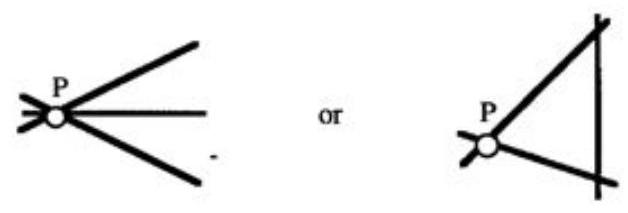
\includegraphics[max width=0.4\textwidth]{images/bo_d3lj80c601uc738kffi0_106_512_1114_628_213_0.jpg}
\end{center}
\hspace*{3em} 

图7.1:3条共点直线或三角形

(b) 每个平面 \(\Pi  \subset  {\mathbb{P}}^{3}\) 与 \(S\) 的交集是以下情形之一：

(i) 一个不可约三次曲线；或

(ii) 一条圆锥曲线和一条直线之并；或

(iii) 三条不同的直线之并.
\end{proposition}

\begin{proof}
(a) 若直线 \(\ell \subset S\) 且 \(P \in \ell\)，则 \(\ell = T_P\ell \subset T_PS\).因此，所有过 \(P\) 点且在 \(S\) 上的直线都包含在切平面 \(T_PS\) 内.由 (b) 可知，这样的直线至多有三条.

(b) 我们必须证明不可能出现重直线的情形.设平面 \(\Pi\) 的方程为 \(T=0\)，\(\Pi\) 中一直线 \(\ell\) 的方程为 \(Z=0\).若 \(\ell\) 是 \(S \cap \Pi\) 的一条重直线，则意味着 \(f\) 具有如下形式：
\[
f = Z^2 \cdot A(X,Y,Z,T) + T \cdot B(X,Y,Z,T),
\]
其中 \(A\) 为线性型，\(B\) 为二次型.此时，曲面 \(S: (f=0)\) 在满足 \(Z=T=B=0\) 的点处是奇异的.这是一个非空集合，因为它是二次型 \(B\) 在直线 \(\ell: (Z=T=0)\) 上的零点集.
\end{proof}

\begin{proposition}
曲面 \(S\) 上至少存在一条直线.
\end{proposition}

\begin{proof}
此命题有多种证明方法.一个经典论证是通过维数计算：\({\mathbb{P}}^{3}\) 中的直线构成一个4维簇，而一条直线 \(\ell\) 要被包含于 \(S\) 上，需要满足4个条件（因为 \(f\) 限制在 \(\ell\) 上是一个三次齐次多项式，其4个系数都必须为零）.要将此论证转化为严格证明，还需要一些工作，因为它先验地只表明直线集的维数 \(\ge 0\)，而非非空（详见 \cite[8.15]{MilesReid_UndergraduateAlgebraicGeometry} 对传统证明及其难点的讨论）.

我们也可以合理地假设该命题成立（即只关注那些包含直线的三次曲面）.现在，我们说明如何通过直接的坐标几何和消元法来证明命题 7.2.证明过程将占用接下来的三页，并分为四个步骤；如果你愿意，可以跳过（直接看命题 7.3）.

\textbf{步骤1（初步构造）} 对 \(S\) 上任意一点 \(P\)，\(S\) 与其切平面 \(T_PS\) 的交线是一个平面三次曲线 \(C = S \cap T_PS\).根据练习 6.7，该曲线在点 \(P\) 处奇异.我们假设 \(C\) 是不可约的，否则 \(P\) 就位于 \(S\) 的一条直线上，命题已然成立.此时，\(C\) 是一个有结点或尖点的三次曲线.我们可以选择适当的 \({\mathbb{P}}^{3}\) 坐标 \((X, Y, Z, T)\)，使得 \(T_PS\) 的方程为 \(T=0\)，\(P = (0,0,1,0)\)，且
\[
C: (XYZ = X^3 + Y^3) \text{ 或 } (X^2Z = Y^3).
\]
对给定的点 \(P \in S\)，交线 \(C\) 是有结点还是有尖点，取决于 \(f\) 在 \(P\) 点的二阶导数矩阵（即 Hessian 矩阵）.练习 7.3 对此有更详细的讨论，并证明了（在特征 \(\neq 2\) 时）尖点情形必在 \(S\) 的某点 \(P\) 处出现.为简便起见，我们在尖点情形下证明命题 7.2；原则上，结点情形的证明方法相同，但消元计算更为复杂（见练习 7.10）.因此，我们假设
\[
f = X^2Z - Y^3 + gT,
\]
其中 \(g = g_2(X,Y,Z,T)\) 是一个二次型.由于 \(S\) 在 \(P\) 点非奇异，我们可以假设 \(g(0,0,1,0) = 1\).

\textbf{步骤2（主要命题陈述）} 考虑 \(C \subset S\) 上的动点 \(P_\alpha = (1, \alpha, \alpha^3, 0)\).过 \(P_\alpha\) 的 \({\mathbb{P}}^{3}\) 中任意一条直线与补平面 \(\Pi: (X=0)\) 交于一点 \(Q = (0,Y,Z,T)\).我们用 \(\alpha\) 和 \(Q\) 的坐标来表示直线 \(P_\alpha Q\) 被包含于 \(S\) 的条件.将 \(f(\lambda P_\alpha + \mu Q)\) 按 \(\lambda\) 和 \(\mu\) 的幂次展开，得到
\[
P_\alpha Q \subset S \iff A(Y,Z,T) = B(Y,Z,T) = C(Y,Z,T) = 0,
\]
其中 \(A, B, C\) 是关于 \((Y, Z, T)\) 的 1, 2, 3 次齐次多项式，其系数与 \(\alpha\) 有关.

\textbf{主要命题}. 存在一个关于 \(\alpha\) 的 27 次首一“结式”多项式 \(R_{27}(\alpha)\)，使得
\[
R(\alpha) = 0 \iff A=B=C=0 \text{ 在 } {\mathbb{P}}^{2} \text{ 中有公共零点 } (\eta:\zeta:\tau).
\]
该命题证明了命题 7.2，因为它意味着对于 \(R\) 的每一个根 \(\alpha\)，都存在平面 \(\Pi\) 中的一点 \(Q = (0:\eta:\zeta:\tau)\)，使得直线 \(P_\alpha Q\) 包含于 \(S\).这里的思路是基于练习 1.10 的标准消元法计算；证明的其余部分将致力于明确写出 \(A, B, C\) 以证明此命题.

\textbf{步骤3（极化形式）} 定义 \(f\) 的极化形式 \(f_1\)，它是一个关于两组变量 \((X,Y,Z,T)\) 和 \((X',Y',Z',T')\) 的多项式，定义如下：
\[
f_1(X,Y,Z,T; X',Y',Z',T') = \frac{\partial f}{\partial X} X' + \frac{\partial f}{\partial Y} Y' + \frac{\partial f}{\partial Z} Z' + \frac{\partial f}{\partial T} T'.
\]
根据切空间的定义（见 (6.4) 和 (6.10)），对于 \(P=(X,Y,Z,T) \in S\) 和 \(P \neq Q=(X',Y',Z',T') \in {\mathbb{P}}^{3}\)，我们显然有
\[
f_1(P;Q) = 0 \iff \text{直线 } PQ \text{ 在点 } P \text{ 处与 } S \text{ 相切.}
\]
显然，
\[
f(\lambda P + \mu Q) = \lambda^3 f(P) + \lambda^2\mu f_1(P;Q) + \lambda\mu^2 f_1(Q;P) + \mu^3 f(Q),
\]
因此，对于 \(P \neq Q \in {\mathbb{P}}^{3}\)，以下四个条件
\[
f(P) = f_1(P;Q) = f_1(Q;P) = f(Q) = 0
\]
是直线 \(\ell = PQ\) 包含于曲面 \(S: (f=0)\) 的充要条件.从几何角度看，这些条件表明 \(\ell\) 在 \(P\) 和 \(Q\) 两点都与 \(S\) 相切，因此 \(f|_\ell\) 在这两点都有重根.由命题 1.8 可推得 \(\ell \subset S\).

对于 \(f = X^2Z - Y^3 + gT\)，其极化形式为
\[
f_1 = 2XZ \cdot X' - 3Y^2 \cdot Y' + X^2 \cdot Z' + g(X,Y,Z,T) \cdot T' + T g_1.
\]
这里 \(g_1 = g_1(X,Y,Z,T; X',Y',Z',T')\) 是以同样方式定义的 \(g\) 的极化形式.由于 \(g\) 是二次型，\(g_1\) 是对称双线性型，满足 \(g_1(P,P) = 2g(P)\).

代入 \(P_\alpha = (1, \alpha, \alpha^3, 0)\) 和 \(Q = (0,Y,Z,T)\)，我们得到直线 \(P_\alpha Q \subset S\) 的方程组为 \(A=B=C=0\)，其中
\begin{align*}
A &= Z - 3\alpha^2 Y + g(1, \alpha, \alpha^3, 0)T, \\
B &= -3\alpha Y^2 + g_1(1, \alpha, \alpha^3, 0; 0,Y,Z,T)T, \\
C &= -Y^3 + g(0,Y,Z,T)T.
\end{align*}

\textbf{步骤4（消元计算）} 现在我们从上述三个方程中消去 \(Y,Z,T\)，并关注 \(\alpha\) 的最高次幂.注意到由于 \(g(0,0,1,0)=1\)，我们有
\[
g(1, \alpha, \alpha^3, 0) = \alpha^6 + \dots = a^{(6)},
\]
其中 \(\dots\) 表示 \(\alpha\) 的低次项.因此，\(a^{(6)}\) 是一个 6 次首一多项式.方程 \(A=0\) 将 \(Z\) 表示为 \(Y\) 和 \(T\) 的线性组合：
\[
Z = 3\alpha^2 Y - a^{(6)}T.
\]
将此代入 \(B\)，并利用 \(g_1\) 的双线性性质，得到
\begin{align*}
B &= -3\alpha Y^2 + g_1(1, \alpha, \alpha^3, 0; 0, Y, 3\alpha^2 Y - a^{(6)}T, T)T \\
  &= b_0 Y^2 + b_1 YT + b_2 T^2,
\end{align*}
其中
\begin{align*}
b_0 &= -3\alpha, \\
b_1 &= g_1(1, \alpha, \alpha^3, 0; 0, 1, 3\alpha^2, 0) = 6\alpha^5 + \dots, \\
b_2 &= g_1(1, \alpha, \alpha^3, 0; 0, 0, -a^{(6)}, 1) = -2\alpha^9 + \dots.
\end{align*}
类似地，将 \(Z\) 的表达式代入 \(C\)，并展开二次型 \(g\)，得到
\begin{align*}
C &= -Y^3 + g(0, Y, 3\alpha^2 Y - a^{(6)}T, T)T \\
  &= c_0 Y^3 + c_1 Y^2T + c_2 YT^2 + c_3 T^3,
\end{align*}
其中
\begin{align*}
c_0 &= -1, \\
c_1 &= g(0, 1, 3\alpha^2, 0) = 9\alpha^4 + \dots, \\
c_2 &= g_1(0, 1, 3\alpha^2, 0; 0, 0, -a^{(6)}, 1) = -6\alpha^8 + \dots, \\
c_3 &= g(0, 0, -a^{(6)}, 1) = \alpha^{12} + \dots.
\end{align*}
现在，根据练习 1.10 的结式理论，\(B\) 和 \(C\) 有公共零点 \((\eta:\tau)\) 当且仅当它们的 Sylvester 行列式为零：
\[
\det \begin{vmatrix}
-3\alpha & 6\alpha^5 & -2\alpha^9 & & \\
& -3\alpha & 6\alpha^5 & -2\alpha^9 & \\
& & -3\alpha & 6\alpha^5 & -2\alpha^9 \\
-1 & 9\alpha^4 & -6\alpha^8 & \alpha^{12} & \\
& -1 & 9\alpha^4 & -6\alpha^8 & \alpha^{12}
\end{vmatrix} = 0.
\]
该行列式是关于 \(\alpha\) 的多项式，不难看出其首项来自于取行列式中每个元素的首项：
\[
\det \begin{vmatrix}
-3\alpha & 6\alpha^5 & -2\alpha^9 & & \\
& -3\alpha & 6\alpha^5 & -2\alpha^9 & \\
& & -3\alpha & 6\alpha^5 & -2\alpha^9 \\
-1 & 9\alpha^4 & -6\alpha^8 & \alpha^{12} & \\
& -1 & 9\alpha^4 & -6\alpha^8 & \alpha^{12}
\end{vmatrix} = \alpha^{27} \cdot \det \begin{vmatrix}
-3 & 6 & -2 & & \\
& -3 & 6 & -2 & \\
& & -3 & 6 & -2 \\
-1 & 9 & -6 & 1 & \\
& -1 & 9 & -6 & 1
\end{vmatrix}
\]
（行列式中的 `2` 应该是 `-2`）经过计算，这个 \(5 \times 5\) 的常数行列式的值为 1，所以
\[
\text{结式} = \alpha^{27} + \dots.
\]
这便完成了主要命题的证明.
\end{proof}

\begin{proposition}
给定一条直线 \(\ell \subset S\)，恰好存在 5 对直线 \((\ell_i, \ell_i')\)，它们是 \(S\) 中与 \(\ell\) 相交的直线，且满足：
\begin{enumerate}
    \item[(i)] 对 \(i=1, \dots, 5\)，\(\ell \cup \ell_i \cup \ell_i'\) 共面；
    \item[(ii)] 对 \(i \neq j\)，\((\ell_i \cup \ell_i') \cap (\ell_j \cup \ell_j') = \varnothing\).
\end{enumerate}
\end{proposition}

\begin{proof}
(摘自 \cite[p. 51]{Beauville_ComplexAlgebraicSurfaces}) 若 \(\Pi\) 是 \({\mathbb{P}}^{3}\) 中任一包含 \(\ell\) 的平面，则 \(\Pi \cap S = \ell \cup C\)，其中 \(C\) 是一条圆锥曲线（因为 \(f|_\Pi\) 可被 \(\ell\) 的方程整除）.该圆锥曲线可以是奇异的，也可以是非奇异的：

\begin{center}
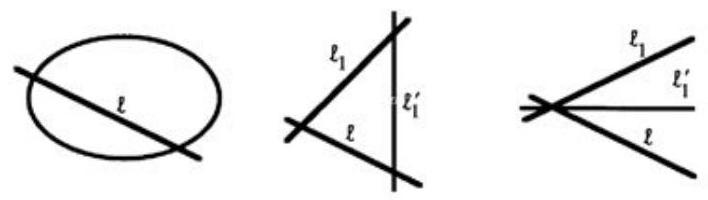
\includegraphics[max width=0.5\textwidth]{images/bo_d3lj80c601uc738kffi0_110_493_393_708_200_0.jpg}
\end{center}
\hspace*{3em} 

图7.2: 直线与圆锥曲线之并

我们必须证明，恰有 5 个不同的平面 \(\Pi_i \supset \ell\) 使得奇异情形（即圆锥曲线分解为两条直线）发生.性质 (ii) 中所述的不同平面内的直线互不相交，这是命题 7.1(a) 的直接推论.

假设 \(\ell\) 的方程为 \(Z=T=0\).那么我们可以将 \(f\) 展开为
\[
f = AX^2 + BXY + CY^2 + DX + EY + F, \quad (*)
\]
其中 \(A,B,C,D,E,F \in k[Z,T]\)，\(A,B,C\) 是线性型，\(D,E\) 是二次型，\(F\) 是三次型.如果我们将此方程视为变量在 \(X,Y\) 中的圆锥曲线，则其退化（即奇异）的条件是判别式为零：
\[
\Delta(Z,T) = \det \begin{pmatrix} 2A & B & D \\ B & 2C & E \\ D & E & 2F \end{pmatrix} = 4ACF + BDE - AE^2 - B^2F - CD^2 = 0.
\]
(这里我们假设特征 \(\neq 2\).在特征 2 的情况下，这是一个简单的练习.)

更准确地说，任何过 \(\ell\) 的平面都由 \(\Pi: (\mu Z = \lambda T)\) 给出.若 \(\mu \neq 0\)，我们可以设 \(\mu=1\)，即 \(Z = \lambda T\).然后用平面 \(\Pi\) 上的齐次坐标 \((X,Y,T)\) 表示，我们有 \(f|_\Pi = T \cdot Q(X,Y,T)\)，其中
\begin{multline*}
Q = A(\lambda,1)X^2 + B(\lambda,1)XY + C(\lambda,1)Y^2 \\
+ D(\lambda,1)TX + E(\lambda,1)TY + F(\lambda,1)T^2.
\end{multline*}
现在，\(\Delta(Z,T)\) 是一个关于 \(Z,T\) 的齐次五次多项式，因此根据代数基本定理（或命题 1.8），它有 5 个根（计重数）.为证明该命题，我们必须证明它没有重根.这同样是 \(S\) 非奇异性的一个推论.

\textbf{命题}. \(\Delta(Z,T)\) 只有单根.

\begin{proof}
假设 \(Z=0\) 是 \(\Delta\) 的一个根，并令 \(\Pi: (Z=0)\) 为对应的平面.我们必须证明 \(\Delta\) 不能被 \(Z^2\) 整除.根据上图，\(\Pi \cap S\) 是三条直线的并.根据这三条直线是否共点，我们可以调整坐标使得：
\begin{itemize}
    \item[(i)] \(\ell: (T=0), \ell_1: (X=0), \ell_1': (Y=0)\)（不共点，构成三角形）；
    \item[(ii)] \(\ell: (T=0), \ell_1: (X=0), \ell_1': (X=T)\)（共点）.
\end{itemize}
在情形 (i) 中，\(f = XYT + Zg\)，其中 \(g\) 是二次型.根据表达式 (*)，这意味着 \(B = T + aZ\)，且 \(Z\) 整除 \(A,C,D,E,F\).因此，在模 \(Z^2\) 的意义下，
\[
\Delta \equiv -B^2F \equiv -T^2F \pmod{Z^2}.
\]
此外，点 \(P=(0,0,0,1) \in S\)，\(S\) 在 \(P\) 点的非奇异性意味着 \(F\) 必须包含形如 \(cZT^2\) 且 \(c \neq 0\) 的项.特别地，\(Z^2\) 不整除 \(F\).因此，\((Z=0)\) 是 \(\Delta\) 的一个单根.

情形 (ii) 的计算是类似的（见习题 7.1）.
\end{proof}
\end{proof}

\begin{corollary}
1. \(S\) 上存在两条不相交的直线 \(\ell, m\).
2. \(S\) 是有理曲面（即与 \({\mathbb{P}}^{2}\) 双有理等价，见 (5.9)）.
\end{corollary}

\begin{proof}
(a) 根据命题 7.3(ii)，只需取 \(\ell_1\) 和 \(\ell_2\).

(b) 考虑 \(S\) 上两条不相交的直线 \(\ell, m\)，并定义如下的有理映射：
\[
\varphi: S \dashrightarrow \ell \times m \quad \text{和} \quad \psi: \ell \times m \dashrightarrow S.
\]
如果 \(P \in {\mathbb{P}}^{3} \setminus (\ell \cup m)\)，则存在唯一一条通过 \(P\) 且同时与 \(\ell\) 和 \(m\) 相交的直线 \(n\)，即
\[
P \in n, \quad \ell \cap n \neq \varnothing, \quad m \cap n \neq \varnothing.
\]
令 \(\Phi(P) = (\ell \cap n, m \cap n) \in \ell \times m\).这定义了一个态射
\[
\Phi: {\mathbb{P}}^{3} \setminus (\ell \cup m) \to \ell \times m,
\]
其在 \((Q,R) \in \ell \times m\) 上的纤维是 \({\mathbb{P}}^{3}\) 中的直线 \(QR\).定义 \(\varphi: S \dashrightarrow \ell \times m\) 为 \(\Phi\) 在 \(S\) 上的限制.

反之，对于 \((Q,R) \in \ell \times m\)，令 \(n\) 为 \({\mathbb{P}}^{3}\) 中的直线 \(n=QR\).根据命题 7.3，与 \(\ell\) 相交的 \(S\) 中的直线只有有限条.因此，对于几乎所有的 \((Q,R)\)，直线 \(n\) 与 \(S\) 交于三点 \(\{P,Q,R\}\)，其中 \(Q \in \ell\) 和 \(R \in m\) 是给定的点.因此，我们通过 \((Q,R) \mapsto P\) 定义了 \(\psi: \ell \times m \dashrightarrow S\).由于 \(P\) 的坐标是 \(Q,R\) 坐标的有理函数，故 \(\psi\) 是一个有理映射.

显然，\(\varphi\) 和 \(\psi\) 互为逆映射.
\end{proof}

\section{寻找所有S上的直线}

我们希望基于命题 7.3 给出的由一条直线 \(\ell\) 和 5 对不相交直线 \((\ell_i, \ell_i')\) 构成的图形，找出 \(S\) 上的所有直线.任何其他直线 \(n \subset S\) 必须与 \(i=1, \dots, 5\) 中的每一对 \((\ell_i, \ell_i')\) 之一恰好相交一次.这是因为在 \({\mathbb{P}}^{3}\) 中，\(n\) 与包含第 \(i\) 对直线的平面 \(\Pi_i\) 相交，而 \(\Pi_i \cap S = \ell \cup \ell_i \cup \ell_i'\).此外，\(n\) 不可能同时与 \(\ell_i\) 和 \(\ell_i'\) 相交，否则将与命题 7.1(a) 矛盾.解决剩余直线问题的关键是以下引理，它告诉我们 \(n\) 由其与 \(\ell_i\) 和 \(\ell_i'\) 中的哪一条相交唯一确定.这里，我们说一条直线 \(n\) 是直线 \(\ell\) 的一条“贯线”（transversal），如果 \(\ell \cap n \neq \varnothing\).

\begin{lemma}
如果 \({\ell}_{1},\ldots ,{\ell}_{4} \subset  {\mathbb{P}}^{3}\) 是四条互相不交的直线，则
\begin{itemize}
    \item 要么这四条直线 \(\ell_i\) 都位于一个光滑二次曲面上，\({\ell}_{1},\ldots ,{\ell}_{4} \subset  Q \subset  {\mathbb{P}}^{3}\).此时，它们有无穷多条公共贯线.
    \item 要么这四条直线 \(\ell_i\) 不位于任何二次曲面上.此时，它们有 1 条或 2 条公共贯线.
\end{itemize}
\end{lemma}

\begin{proof}
存在一个光滑二次曲面 \(Q \supset \ell_1, \ell_2, \ell_3\).对此有多种证明方法（见练习 7.2）.

\begin{center}
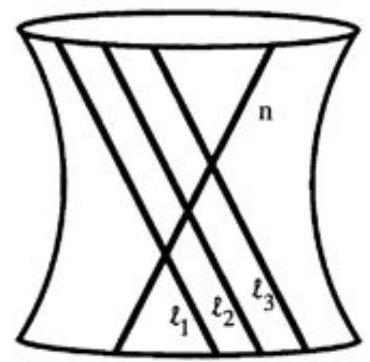
\includegraphics[max width=0.2\textwidth]{images/bo_d3lj80c601uc738kffi0_112_658_391_370_362_0.jpg}
\end{center}
\hspace*{3em} 

图7.3: 过三条不交直线的二次曲面

那么，在适当的坐标系中，\(Q\) 的方程为 \(XT-YZ=0\)，且 \(Q\) 上有两族直纹，或称母线.任何贯穿 \(\ell_1, \ell_2, \ell_3\) 的直线都必须位于 \(Q\) 中，因为它在 \(Q\) 上有三个点.现在，如果 \(\ell_4 \not\subset Q\)，则 \(\ell_4 \cap Q\) 为一个或两个点.通过这些点的另一族母线即为 \(\ell_1, \dots, \ell_4\) 的所有公共贯线.
\end{proof}

\section{27条直线}

设 \(\ell\) 和 \(m\) 是 \(S\) 中两条不相交的直线.如前所述，\(m\) 恰好与 5 对和 \(\ell\) 相交的直线中的每一对的一条相交.通过重新编号，我们假设 \(m\) 与 \(\ell_i\) 相交，其中 \(i=1, \dots, 5\).我们引入以下记号来表示与 \(\ell\) 或 \(m\) 相交的直线：

\begin{center}
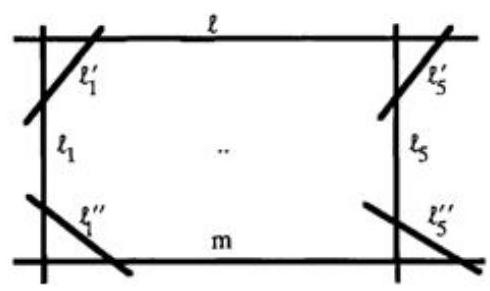
\includegraphics[max width=0.3\textwidth]{images/bo_d3lj80c601uc738kffi0_112_603_1306_490_291_0.jpg}
\end{center}
\hspace*{3em} 

图7.4: \(S_3 \subset {\mathbb{P}}^3\) 上的直线构型

因此，与 \(m\) 相交的 5 对直线是 \((\ell_i, \ell_i'')\)，其中 \(i=1, \dots, 5\).根据命题 7.3(ii) 对 \(m\) 的应用，对于 \(i \neq j\)，直线 \(\ell_i''\) 不与 \(\ell_j\) 相交.另一方面，\(S\) 中的每条直线必须与 \(\ell, \ell_j\) 或 \(\ell_j'\) 中的一条相交，因此 \(\ell_i''\) 必与 \(\ell_j'\) 相交，其中 \(i \neq j\).

\begin{proposition}
(I) 如果 \(n \subset S\) 是除这 17 条（\(\ell, m, \ell_i, \ell_i', \ell_i''\)）之外的任意直线，则 \(n\) 恰好与 \(\ell_1, \dots, \ell_5\) 中的三条相交.

(II) 反之，对于集合 \(\{1,2,3,4,5\}\) 中任意选择的 3 个元素 \(\{i,j,k\}\)，都存在唯一一条直线 \(\ell_{ijk} \subset S\) 与 \(\ell_i, \ell_j, \ell_k\) 相交.
\end{proposition}

\begin{proof}
(I) 给定 \(S\) 中的四条不相交直线，显然它们不可能都位于同一个二次曲面 \(Q\) 上，否则 \(Q \subset S\)，这与 \(S\) 的不可约性矛盾.

如果 \(n\) 与 \(\ge 4\) 条 \(\ell_i\) 相交，则根据引理 7.5，\(n\) 必为 \(\ell\) 或 \(m\)，这产生矛盾.如果 \(n\) 与 \(\le 2\) 条 \(\ell_i\) 相交，则它必与 \(\ge 3\) 条 \(\ell_i'\) 相交.因此，它与 \(\ell_2', \ell_3', \ell_4', \ell_5'\) 或 \(\ell_1, \ell_3', \ell_4', \ell_5'\) 之一相交.但如上所述，\(\ell\) 和 \(\ell_1''\) 是五条不相交直线 \(\ell_2', \ell_3', \ell_4', \ell_5', \ell_1\) 的两条公共贯线.因此，再次根据引理 7.5，如果 \(n\) 与其中 \(\ge 4\) 条相交，则 \(n\) 必为 \(\ell\) 或 \(\ell_1''\).这同样是矛盾.

(II) 根据命题 7.3，有 10 条直线与 \(\ell_1\) 相交.目前我们只考虑了其中的 4 条（即 \(\ell, \ell_1', m, \ell_1''\)）.其余 6 条直线必须恰好与剩下的 4 条直线 \(\ell_2, \dots, \ell_5\) 中的两条相交.而这样的选择恰好有 \(6 = \binom{4}{2}\) 种，因此它们必须全部出现.
\end{proof}

这给出了 \(S\) 上的所有直线为：
\[
\{\ell, m, \ell_i, \ell_i', \ell_i'', \ell_{ijk}\},
\]
其总数为
\[
1 + 1 + 5 + 5 + 5 + 10 = 27.
\]

\section{直线的构型}

另一种表述是，\(S\) 上的直线是 \(\ell, \ell_1, \dots, \ell_5, \ell_1', \dots, \ell_5'\)，以及另外 16 条与 \(\ell_1, \dots, \ell_5\) 相交奇数次的直线：
\begin{itemize}
    \item \(\ell_i''\) 只与 \(\ell_i\) 相交.
    \item \(\ell_{ijk}\) 只与 \(\ell_i, \ell_j, \ell_k\) 相交.
    \item \(m\) 与所有的 \(\ell_1, \dots, \ell_5\) 相交.
\end{itemize}
在我引入的记号中，很容易看出 \(S\) 的 27 条直线之间的相交关系如下：
\begin{itemize}
    \item \(\ell\) 与 \(\ell_1, \dots, \ell_5, \ell_1', \dots, \ell_5'\) 相交.
    \item \(\ell_1\) 与 \(\ell, m, \ell_1', \ell_1''\) 相交，并与 6 条 \(\ell_{1jk}\)（其中 \(\{j,k\} \subset \{2,3,4,5\}\)）相交.
    \item \(\ell_1'\) 与 \(\ell, \ell_1, \ell_j''\)（\(j \neq 1\)，4种选择）相交，并与 \(\ell_{ijk}\)（\(\{i,j,k\} \subset \{2,3,4,5\}\)，4种选择）相交.
    \item \(\ell_1''\) 与 \(m, \ell_1, \ell_j'\)（\(j \neq 1\)，4种选择）相交，并与 \(\ell_{ijk}\)（\(\{i,j,k\} \subset \{2,3,4,5\}\)，4种选择）相交.
    \item \(\ell_{123}\) 与 \(\ell_1, \ell_2, \ell_3, \ell_{145}, \ell_{245}, \ell_{345}, \ell_4', \ell_5', \ell_4'', \ell_5''\) 相交.
\end{itemize}
该组合构型有多种不同的表示形式，其中一些比此处给出的更具对称性；例如参见 \cite[pp. 122-128, 151-152]{SempleRoth_IntroductionToAlgebraicGeometry}.

\section{第7章习题}

\begin{exercise}
证明命题 7.3 中所声明的情形 (ii).[提示：如同情形 (i) 的证明，\(f = X(X-T)T + Zg\)，因此 \(A = T+aZ, D = -T^2 + Z\ell\)，其中 \(\ell\) 是线性的.于是 \(Z \mid B,C,E,F\)，且 \(Z \nmid D\).此外，\(S\) 在点 \((0,1,0,0)\) 处的非奇异性意味着 \(C=cZ\) 且 \(c \neq 0\).现在计算 \(\Delta(Z,T) \pmod{Z^2}\).]
\end{exercise}

\begin{exercise}
证明给定三条互相不交的直线 \(\ell_1, \ell_2, \ell_3 \subset {\mathbb{P}}^{3}\)，存在一个非奇异的二次曲面 \(Q \supset \ell_1, \ell_2, \ell_3\).[提示：在每条直线 \(\ell_i\) 上取三个点 \(P_i, P_i', P_i''\)，并如 (1.11) 或 (2.4) 所示，证明至少存在一个过这九个点的二次曲面 \(Q\).由此可知 \(\ell_i \subset Q\).现在证明 \(Q\) 不可能是奇异的：例如，如果 \(Q\) 是一对平面，会发生什么？]
\end{exercise}

\begin{exercise}[Hessian 矩阵]
设 \(f = f_d(x_0, \dots, x_n)\) 是关于 \(x_0, \dots, x_n\) 的 \(d\) 次齐次多项式，定义了超曲面 \(V: (f=0) \subset {\mathbb{P}}^{n}\).为简便起见，假设域的特征 \(\neq 2\) 且不整除 \(d-1\).记 \(f_{x_i} = \partial f/\partial x_i\) 和 \(f_{x_ix_j} = \partial^2 f/\partial x_i \partial x_j\) 分别为 \(f\) 的一阶和二阶偏导数.\(f\) 在点 \(P \in {\mathbb{P}}^{n}\) 处的泰勒展开为
\[
f = f(P) + f^{(1)}(x) + f^{(2)}(x) + \dots,
\]
其中 \(f^{(1)}\) 和 \(f^{(2)}\) 分别是线性和二次齐次多项式：
\[
f^{(1)} = \sum f_{x_i}(P) \cdot x_i \quad \text{和} \quad f^{(2)} = \frac{1}{2} \sum f_{x_ix_j}(P) \cdot x_i x_j.
\]
如果 \(P \in V\) 是一个奇异点，那么 \(f(P)\) 和 \(f^{(1)}\) 在 \(P\) 处为零，\(V\) 或 \(f\) 在 \(P\) 附近的性质由二次型 \(f^{(2)}\) 在二阶近似下决定.类似地，如果 \(P \in V\) 是一个非奇异点，那么 \(f\) 限制在超平面 \(T_PV\) 上的性质（或奇异超平面截面 \(V \cap T_PV\) 的性质）由 \(f^{(2)}\) 决定.定义 \(f\) 关于坐标 \(x_0, \dots, x_n\) 的 Hessian 矩阵为 \(H(f) = H(f,x) = \{f_{x_ix_j}\}_{i,j}\)，Hessian \(h(f) = h(f,x)\) 定义为其行列式 \(h(f) = \det H(f)\).

(i) 设 \(x_i' = \sum a_{ij}x_j\) 为一个射影坐标变换，\(A = (a_{ij})\) 是一个非奇异的 \((n+1) \times (n+1)\) 矩阵.若 \(g(x') = f(Ax)\)，证明 Hessian 矩阵的变换规律为
\[
H(g,x') = ({}^tA) H(f,x) A,
\]
其中 \({}^tA\) 为转置矩阵.由此推导出 \(h(g,x') = (\det A)^2 h(f,x)\).

(ii) 考虑如 (5.5) 中所述的仿射片 \(V_{(i)} \subset {\mathbb{A}}_{(i)}^{n}\)，设 \(P \in V_{(i)}\) 为非奇异点，\(\Pi = T_P V_{(i)}\) 为仿射切平面.记 \(\varphi\) 为定义方程 \(f/x_i^d\) 在 \(\Pi\) 上的限制.证明 \(\varphi\) 在 \(P\) 处的泰勒展开以一个非退化的二次型 \(\varphi^{(2)}\)（在 \(n-1\) 个变量中）开始，当且仅当 \(h(f)(P) \neq 0\).
[提示：利用 (i) 化简为 \(P=(1,0,\dots,0)\) 和 \(T_PV: (x_1=0)\).此时 \(\varphi^{(2)}\) 是射影 Hessian 矩阵 \(H(f)\) 的右下角 \((n-1) \times (n-1)\) 子矩阵.用 \(f_{x_i}(P)=0\)（\(i \neq 1\)）和欧拉公式 \(\sum_j f_{x_ix_j} x_j = (d-1)f_{x_i}\) 证明矩阵 \(H(f)\) 在第 0 行和第 0 列中恰有一个非零元.参见 \cite[p. 116]{Fulton_AlgebraicCurves}.]

(iii) 设 \(C: (f=0) \subset {\mathbb{P}}^{2}\) 为非奇异平面三次曲线.由 (ii) 推导出 \(P \in C\) 是一个拐点当且仅当 \(H(f)(P)=0\).Bézout 定理表明 \((f=H(f)=0) \subset {\mathbb{P}}^{2}\) 非空（参见 (1.9) 及 \cite[p. 112]{Fulton_AlgebraicCurves}）.

(iv) 设 \(S: (f=0) \subset {\mathbb{P}}^{3}\) 为非奇异三次曲面.对 \(P \in S\)，证明若 \(P\) 不在 \(S\) 的任何直线上，则交线 \(S \cap T_PS\) 为尖点三次曲线当且仅当 \(H(f)(P)=0\).由此推断存在尖点三次截面，正如命题 7.2 证明步骤 1 所需.
\end{exercise}

\begin{exercise}
(i) 证明若 \(P\) 是三次曲面 \(S\) 的一个奇异点，则至少存在一条直线 \(\ell \subset S\) 经过 \(P\)（且“一般情况下”有 6 条）.

(ii) 如果 \(X \subset {\mathbb{P}}^{4}\) 是一个非奇异的三次超曲面（三次三维簇）且 \(P \in X\)，那么至少存在一条直线 \(\ell \subset X\) 经过 \(P\)（通常有 6 条）.[提示：用 \(P=(1,0,\dots,0)\) 的坐标写出 \(X\) 的方程.]
\end{exercise}

\begin{exercise}
证明推论 7.4(b) 中的有理映射 \(\varphi: S \dashrightarrow \ell \times m\) 实际上是一个态射.证明它将 \(S\) 上的 5 条直线收缩为点.
\end{exercise}

\begin{exercise}
找出对角三次曲面（Fermat 三次曲面）
\[
S: (X^3 + Y^3 + Z^3 + T^3 = 0) \subset {\mathbb{P}}^{3}
\]
上的全部 27 条直线，可用形如 \((X = \rho Y)\) 的平面来寻找，其中 \(\rho^3=-1\).
\end{exercise}

\begin{exercise}
设 \(S \subset {\mathbb{P}}^{3}\) 是由 \(S: (f=0)\) 给出的三次曲面，其中
\[
f(X,Y,Z,T) = ZX^2 + TY^2 + (Z-d^2T)(Z-e^2T)(Z-f^2T),
\]
\(d,e,f\) 是 \(k\) 中不同的非零元素.\(\ell \subset S\) 是由 \(Z=T=0\) 给出的直线.通过类似命题 7.3 中考虑经过 \(\ell\) 的动平面，写出与 \(\ell\) 相交的 \(S\) 上的 10 条直线的方程.
\end{exercise}

\begin{exercise}[由 R. Casdagli 提出]
考虑在仿射坐标下由下式给出的三次曲面 \(S_{(0)} \subset {\mathbb{R}}^{3}\)：
\[
x^2 + y^2 + z^2 - 2xyz = 1 + \lambda^2, \quad (*)
\]
其中 \(\lambda \in \mathbb{R}, \lambda > 0\) 是常数.(i) 通过将 \((*)\) 重写为
\[
(x-yz)^2 = (y^2-1)(z^2-1) + \lambda^2,
\]
证明 \(S_{(0)}\) 有 4 个通向无穷远的管状区域.另一方面，相应的射影曲面 \(S \subset {\mathbb{P}}_{\mathbb{R}}^{3}\) 在无穷远处与三条直线 \(XYZ=0\) 相交.利用此信息描述 \(S\) 的拓扑结构.

(ii) 将 \((*)\) 视为以 \(z\) 为参数的 \((x,y)\) 平面上的动圆锥曲线方程，证明与平面 \((Z=0)\) 渐近相交的四对 \(S_{(0)}\) 上的直线由下式给出：
\begin{align*}
z = \mu, &\quad x = (\mu \pm \sqrt{\mu^2-1})y \\
z = -\mu, &\quad x = (-\mu \pm \sqrt{\mu^2-1})y;
\end{align*}
以及另外 8 条实直线，例如
\[
z=1, \quad x-y = \pm\lambda; \quad \text{和} \quad z=-1, \quad x+y = \pm\lambda,
\]
其中 \(\mu^2 = 1+\lambda^2\).
用计算机图形学或制作石膏模型来展示曲面 \(S_{(0)}\) 在 \({\mathbb{R}}^{3}\) 中的形态及其 24 条实直线.
\end{exercise}

\begin{exercise}[所有直线均为有理线的情形]
假设域 \(k\) 的特征 \(\neq 2\).设 \(S: (f=0)\) 是一个非奇异三次曲面，满足
\[
f = A(X,Y)T - B(X,Y)Z + (\text{含 } Z,T \text{ 的次数} \ge 2 \text{ 的项}).
\]
则 \(S\) 包含直线 \(\ell: (Z=T=0)\)，且在点 \(P=(1,\lambda,0,0)\) 处的切平面为 \(T_PS: A(1,\lambda)T = B(1,\lambda)Z\).

(i) 利用 \((X,Y)\) 和 \((Z,T)\) 的线性坐标变换，将 \(A,B\) 化简为 \(A=X^2+\Delta Y^2, B=XY\)（其中 \(\Delta \in k\)）；若 \(\Delta\) 是完全平方，则可化为 \(A=X^2, B=Y^2\).

(ii) 假设 \(S\) 也包含直线 \(m: (X=Y=0)\)，并且为简化符号，设 \(A=X^2, B=Y^2\).令 \(\ell_i\)（\(i=1,\dots,5\)）为 \(\ell\) 和 \(m\) 的 5 条公共贯线，记 \(P_i = (1, \lambda_i, 0, 0) = \ell_i \cap \ell\) 为 \(\ell\) 与 \(\ell_i\) 的交点.证明
\[
\ell_i: (Y = \lambda_i X, T = \lambda_i^2 Z) \quad \text{for } i=1,\dots,5,
\]
并且
\[
f = X^2T - Y^2Z + X(\sigma_5 Z^2 + \sigma_3 ZT + \sigma_1 T^2) - Y(\sigma_4 Z^2 + \sigma_2 ZT + T^2),
\]
其中 \(\sigma_1, \dots, \sigma_5\) 是 \(\lambda_1, \dots, \lambda_5\) 的初等对称多项式.

(iii) 求 \(S\) 上剩余的直线.[提示：\(\ell_i'\) 和 \(\ell_i''\) 包含在你已知的平面中.按照 (7.6) 中的论证，不难证明每条与 \(\ell_1, \ell_2, \ell_3\) 三条线相交的直线都可表示为 \((\tau_2 Z+T):X = (\tau_3 Z+\tau_1 T):Y = \alpha:\beta\)，其中 \(\tau_i\) 是 \(\lambda_1, \lambda_2, \lambda_3\) 的初等对称多项式.]
\end{exercise}

\begin{exercise}
本练习适合喜欢大量计算的读者，或有计算机代数系统辅助者.如果一个非奇异三次曲面 \(S\) 有一个结点三次曲线 \(C\) 作为截面，其方程可写为
\[
f = XYZ - X^3 - Y^3 + Tg.
\]
设 \(P_\alpha = (\alpha, \alpha^2, 1+\alpha^3, 0)\)（\(\alpha \neq 0, \infty\)）是 \(C\) 上的动点，及 \(Q=(0,Y,Z,T)\).然后按照命题 7.2 步骤 3，将 \(f(\lambda P_\alpha + \mu Q)\) 展开为 \(f\) 的极化形式，证明直线 \(P_\alpha Q \subset S\) 当且仅当 \(A=B=C=0\)，其中
\begin{align*}
A &= (-3\alpha^2+1)Y + \alpha^2 Z + g(\alpha, \alpha^2, 1+\alpha^3, 0)T; \\
B &= \alpha YZ - 3\alpha^2 Y^2 + g_1(\alpha, \alpha^2, 1+\alpha^3, 0; 0,Y,Z,T)T; \\
C &= -Y^3 + g(0,Y,Z,T)T.
\end{align*}
证明存在一个关于 \(\alpha\) 的 27 次“结式”多项式 \(R_{27}(\alpha)\)，使得对于 \(\alpha \neq 0\)，
\[
R(\alpha) = 0 \iff A=B=C=0 \text{ 在 } {\mathbb{P}}^{2} \text{ 中有公共零点 } (\eta:\zeta:\tau).
\]
[提示：从 \(A=0\) 解出 \(Z\)（这会在分母中引入 \(\alpha^2\)），将 \(Z\) 代入 \(B\) 和 \(C\)，得到关于 \(Y,T\) 的二次和三次二元多项式，然后用 Sylvester 行列式消去 \(Y,T\).此处的难点在于，当 \(\alpha \to 0\) 或 \(\alpha \to \infty\) 时，\(P_\alpha\) 趋于结点，此时 \(A,B,C\) 有平凡公共解，导致结式的首项和末项系数计算变得复杂.你需要仔细计算以确定其确切次数和系数.]
\end{exercise}


\chapter{结语}


本节不计入考试，但其中一些主题可能对学生仍有参考价值.

\section{现代学科的历史与社会学}

\section{8.1 引言}

在过去三十年左右，代数几何在数学界所处的位置类似于数学在整个世界中的地位，既受尊敬又令人畏惧，远多于被理解.与此同时，我经常被英国同事或华威大学的研究生问到的“服务性”问题通常都很基础:一般来说，这些问题要么在本书中有所涉及，要么在[Atiyah和Macdonald]中有所涵盖.以下内容是对该学科近期发展的一个观点，试图解释这一悖论.我不假装客观.

\section{8.2 史前阶段}

代数几何在19世纪由多个不同来源发展而来.首先是几何传统本身:射影几何(以及当时拿破仑时代军方极感兴趣的描绘几何)、为自身目的研究曲线和曲面、构型几何；然后是复函数理论，将紧致黎曼曲面视为代数曲线，并从其函数域纯代数地重构它.在此基础上，代数曲线与数域整数环之间的深刻类比，以及代数和几何中不变量理论语言的需求，这在20世纪初抽象代数的发展中起到了重要作用.

20世纪的最初几十年见证了深刻的分裂.一方面，是研究曲线和曲面的几何传统，尤其由才华横溢的意大利学派推动；除了自身相当可观的成就外，这一传统在拓扑学和微分几何的发展中起到了重要的激励作用，但越来越依赖于“几何直觉”的论证，甚至连大师们也无法严格维持其严谨性.另一方面，新兴的交换代数力量正在奠定基础并提供证明技术.两种方法差异的一个例子是Chow与van der Waerden之间的争论，后者严格证明了参数化给定次数和属的空间曲线的代数簇的存在，而Severi则终其一生创造性地使用此类参数空间，并在晚年痛恨代数学家(尤其是非意大利人！)闯入他的领域，尤其是暗示他所在学派的工作缺乏严谨性.

\section{8.3 严谨性，第一波浪潮}

继希尔伯特和埃米·诺特引入抽象代数后，van der Waerden、Zariski和Weil在1920年代和1930年代为代数几何奠定了严谨的基础(van der Waerden的贡献常被忽略，显然是因为战后初期包括一些顶尖代数几何学家在内的数学家认为他是纳粹合作者).

他们方案的核心之一是使代数几何能在任意域上工作.在这方面，一个关键的基础性难题是你不能仅仅将簇定义为点集:如果你从一个定义在给定域 \(k\) 上的簇 \(V \subset  {\mathbb{A}}_{k}^{n}\) 开始，那么 \(V\) 不仅仅是 \({k}^{n}\) 的一个子集；你还必须允许 \(V\) 的 \(K\) -值点，针对域扩张 \(k \subset  K\) (参见(8.13, c)的讨论).这也是符号 \({\mathbb{A}}_{k}^{n}\) 的由来，表示簇 \({\mathbb{A}}^{n}\) 的 \(k\) -值点，期望其存在独立于指定域 \(k\) .

允许基域在论证过程中变化的必要性极大地增加了技术和概念上的难度(更不用说符号了).然而，到1950年左右，Weil的基础体系被接受为规范，以至于传统几何学家(如Hodge和Pedoe)感到必须以此为基础编写著作，我认为这大大降低了他们著作的可读性.

\section{8.4 格罗滕迪克时代}

从大约1955年到1970年，代数几何领域由巴黎数学家主导，先是塞尔(Serre)，随后尤其是格罗滕迪克(Grothendieck)及其学派.格罗滕迪克方法的影响力不容低估，尤其是在其方法在某种程度上已不再流行的今天.这一时期取得了巨大的概念和技术进步，得益于方案(scheme，比簇更一般，参见下文(8.12-14))概念的系统应用，代数几何几乎吸收了拓扑学、同调代数、数论等领域的所有进展，甚至在这些领域的发展中发挥了主导作用.格罗滕迪克本人于1970年前后在四十出头时退出了学术舞台，这无疑是一大悲剧性损失(他最初因抗议科学军事资助而离开了IHES).作为一名实践中的代数几何学家，我深刻感受到这一时期发展起来的强大理论工具体系，其中许多仍待以通俗易懂的方式整理成文.

另一方面，格罗滕迪克的人格崇拜带来了严重的副作用:许多毕生致力于掌握魏尔(Weil)基础理论的人遭受了排斥和羞辱，据我所知，只有一两人适应了新的语言；整整一代学生(主要是法国人)被洗脑，愚昧地认为不能用高深抽象形式主义包装的问题不值得研究，因此被排除在数学家自然的发展路径之外——即从一个自己能处理的小问题出发，逐步向外探索.(我实际上知道有一篇关于三次曲面算术的论文最初未被考虑，理由是“构造的自然背景是在一般局部诺特环拓扑空间上”.这绝非玩笑.)当时许多学生似乎没有比研读《EGA》(《代数几何基础》)更高的志向.纯粹为范畴论而学(无疑是所有智力追求中最贫瘠的之一)也始于此时；格罗滕迪克本人不必为此负责，因为他自己对范畴的运用在解决问题上非常成功.

时尚此后又发生了反向转变.在法国最近的一次会议上，我评论了态度的变化，得到的讽刺回答是“但扭曲三次曲线是一个非常好的前代表函子例子”.我了解到，现在负责管理法国科研经费的一些数学家曾在这段知识恐怖时期受苦，因此CNRS科研项目的申请经常被包装得尽量减少与代数几何的关联.

除了极少数能够跟上节奏并存活下来的格罗滕迪克学生外，最持久受益于格罗滕迪克思想并最有效传播这些思想的人，都是间接受其影响的:哈佛学派(通过扎里斯基(Zariski)、芒福德(Mumford)和M.阿廷(M. Artin))，莫斯科的沙法列维奇(Shafarevich)学派，或许还有日本的交换代数学派.

\section{8.5 大爆炸}

历史并未在1970年代初终结，代数几何自那时以来也未曾减少时尚的波动.1970年代，尽管几个大派系各有其特殊兴趣(芒福德与模空间的紧化，格里菲斯(Griffiths)的霍奇理论和代数曲线学派，德利涅(Deligne)与簇的上同调“权重”，沙法列维奇与K3曲面，饭高(Iitaka)及其追随者在高维簇分类等)，我认为我们基本上都相信自己在研究同一学科，代数几何仍是一个整体(实际上还在殖民数学的邻近领域).也许正是因为有一两位专家能够掌握该学科的全部范围，这才成为可能.

到1980年代中期，情况发生了变化，代数几何目前似乎分裂为十多个相互交流有限的学派:曲线与阿贝尔簇，代数曲面与唐纳森理论，三维簇及高维分类，K理论与代数循环，交叉理论与计数几何，一般上同调理论，霍奇理论，特征 \(p\) ，算术代数几何，奇点理论，数学物理的微分方程，弦理论，计算机代数的应用等.

\section{附加脚注与高深评论}

本节混合了基础与高级主题；由于部分内容是对使用本书作为教材的大学教师的“忠告”，或引导高级学生避免学科陷阱，部分材料可能显得晦涩难懂.

\section{8.6 选题}

本书中涉及的主题和示例部分是基于计算难度小和计算简便的实用考虑而选择的.然而，它们也暗示了“簇的分类”:关于圆锥曲线的材料在某种意义上适用于所有有理曲线，而三次曲面是最基本的del Pezzo有理曲面例子.带有群运算的三次曲线是阿贝尔簇(Abelian varieties)的例子；事实(2.2)表明非奇异三次曲线不是有理的，这是分类的第一步.两个平面圆锥曲线的交点(1.12-14)和习题5.6中提到的两个二次曲面的交点也可以纳入类似的模式，其中两个二次曲面的交点在 \({\mathbb{P}}_{k}^{4}\) 中提供了另一类del Pezzo曲面，而两个二次曲面交点上的直线族在 \({\mathbb{P}}_{k}^{5}\) 中提供了二维阿贝尔簇.

曲线的属以及第46页表格中分为三种情况的划分，简而言之就是分类.我本想包含更多关于曲线属的内容，特别是如何用拓扑欧拉示性数或代数几何中的交数来计算属，这些是年轻几何学家必做的五指练习.然而，这些内容足以单独构成一门本科课程，椭圆曲线的复分析理论也是如此.

\section{8.7 计算与理论}

关于这些讲义中的方法，另一点是相当强调那些可以通过显式计算处理的情况.当一般理论证明某种构造的存在时，用显式坐标表达来实现它是一个有益的练习，有助于保持对现实的把握，这也适合本科教材.然而，这不应掩盖理论实际上是为处理复杂情况设计的事实，在那些情况下显式计算往往无法提供任何信息.

\section{8.8 实数域与 \(\mathbb{C}\)}

对实数领域感兴趣的读者可能会失望，因为在 \(§{81} - 2\) 中对 \(\mathbb{R}\) 的处理在 \(§3\) 中让位于对任意域 \(k\) 的讨论，且通常假设该域是代数闭的.我建议这类读者坚持下去；实数几何与复数几何之间存在许多联系，其中一些会令人惊讶.询问实簇的实点是一个非常困难的问题，在代数几何中属于少数兴趣；无论如何，全面了解其复点通常是必要的前提.实数域与 \(\mathbb{C}\) 上的几何之间的另一个直接联系是， \(n\) 维非奇异复簇是 \({2n}\) 维实流形——例如，代数曲面是构造光滑4维流形的主要来源.

除了这些相当明显的联系，还有更微妙的关系，例如:(a) 平面曲线在 \(C \subset  {\mathbb{C}}^{2}\) 上的奇点通过与小球边界的交叉在 \({S}^{3}\) 中产生结；(b) 彭罗斯扭量子构造将带有特殊黎曼度量的4维流形视为一个4维复簇的实值点集，该复簇参数化复3维簇上的有理曲线(因此我们所处的实4维球面 \({S}^{4}\) 可以被识别为复Grassmannian \(\operatorname{Gr}\left( {2,4}\right)\) 中 \({\mathbb{P}}_{\mathbb{C}}^{3}\) 直线的实点集).

\section{8.9 正则函数与层}

已经正确理解了簇 \(X\) 上有理函数 \(f \in  k\left( X\right)\) 的概念以及在点 \(P \in  X\) 处的正则性 \(f\) ((4.7)和(5.4))的读者，对结构层 \({\mathcal{O}}_{X}\) 已有相当直观的认识.对于开集 \(U \subset  X\) ，正则函数的集合是 \(U \rightarrow  k\)

\[
{\mathcal{O}}_{X}\left( U\right)  = \{ f \in  k\left( X\right)  \mid  f\text{ is regular }\forall P \in  U\}  = \mathop{\bigcap }\limits_{{P \in  U}}{\mathcal{O}}_{X,P}
\]

是域 \(k\left( X\right)\) 的子环.层 \({\mathcal{O}}_{X}\) 仅仅是环族 \({\mathcal{O}}_{X}\left( U\right)\) ，当 \(U\) 遍历 \(X\) 的开集时.显然，局部环 \({\mathcal{O}}_{X,P}\) (定义见(4.7)和(5.4))的任一元素在某个包含 \(P\) 的邻域 \(U\) 内是正则的，因此有 \({\mathcal{O}}_{X,P} = \mathop{\bigcup }\limits_{{U \ni  P}}{\mathcal{O}}_{X}\left( U\right)\) .仅此而已；有一个固定的有理截面集合 \(k\left( X\right)\) ，而层在开集 \(U\) 上的截面就是在每个 \(P \in  U\) 处满足正则性条件的有理截面.

该语言足以描述带Zariski拓扑的不可约簇上的任意无挠层.当然，如果 \(X\) 是可约的，或者你想处理更复杂的层，或使用复拓扑，则需要层的完整定义.

\section{8.10 全局定义的正则函数}

如果 \(X\) 是射影簇，那么在每个 \(P \in  X\) 处正则的有理函数 \(f \in  k\left( X\right)\) 只有常数.这是射影簇的一般性质，类似于一复变量函数中的Liouville定理；对于定义在 \(\mathbb{C}\) 上的簇，它源于紧性和最大模原理( \(\left( {X \subset  {\mathbb{P}}_{\mathbb{C}}^{n}}\right.\) 在复拓扑下是紧的，因此全局全纯函数在 \(X\) 上的模必须取得最大值)，但在代数几何中，从头证明这一点出乎意料地困难(参见例如[Hartshorne, I.3.4]；本质上是一个有限性结果，涉及相干上同调群的有限维性).

\section{8.11 射影代数几何的惊人充分性}

Weil对簇的抽象定义(仿射代数集沿同构开集粘合而成)在(0.4)中曾简要提及，并且用层的语言处理起来相当容易.有了这个，单纯考虑嵌入在固定环境空间 \({\mathbb{P}}_{k}^{N}\) 中的簇的想法乍看之下似乎过于限制.我想简要描述一下现代对此问题的看法.

\section{(a) 极化与正性}

首先，簇通常按同构考虑，因此说一个簇 \(X\) 是射影的，意味着 \(X\) 可以嵌入某个 \({\mathbb{P}}^{N}\) ，即同构于如(5.1-7)中所述的闭子簇 \(X \subset  {\mathbb{P}}^{N}\) .拟射影意味着同构于 \({\mathbb{P}}^{N}\) 的局部闭子簇，即射影簇的一个开稠密子集；射影性包含完备性的性质，即 \(X\) 不能作为任何更大簇的稠密开集嵌入.

实际嵌入的选择 \(X \hookrightarrow  {\mathbb{P}}^{N}\) (或非常充足的线丛 \({\mathcal{O}}_{X}\left( 1\right)\) ，其截面将作为 \({\mathbb{P}}^{N}\) 的齐次坐标)通常称为极化，我们用 \(\left( {X,{\mathcal{O}}_{X}\left( 1\right) }\right)\) 表示已做出该选择.除了完备性外，射影簇 \(X \subset  {\mathbb{P}}^{N}\) 满足一个关键的“正次数”条件:若 \(V \subset  X\) 是一个 \(k\) 维子簇，则 \(V\) 与一般线性子空间 \({\mathbb{P}}^{N - k}\) 的交点数为正且有限.反过来，Kleiman判据指出，若一个完备簇上的线丛 \(X\) 在每条曲线 \(C \subset  X\) 上的次数始终大于零(即 \(\geq  \varepsilon\) -(对 \(C\) 的任何合理度量))，则该线丛的某个倍数可用于提供 \(X\) 的射影嵌入.这种正性与复流形上的Kähler度量(与复结构兼容的黎曼度量)选择密切相关.因此，我们将射影性理解为一种“正定性”.

\section{(b) 充分性}

令人惊讶的是，许多代数几何问题都能在射影簇框架内得到解答.前文(8.2)提到的Chow簇构造就是一个例子；另一个是1960年代Mumford的工作，他构造了Picard簇和许多模空间作为拟射影簇(概形).Mori理论(对与有理性相关的簇分类的重要概念进展负责，见[Kollár])是最新的例子；其中的思想和技术本质上不可避免地是射影性的.

\section{(c) 抽象簇的不足}
.
曲线和非奇异曲面自动是拟射影的；但存在非拟射影的抽象簇(奇异曲面，或维数为 \(\geq  3\) 的非奇异簇).然而，如果你需要这些构造，几乎肯定也会需要Moishezon簇(M. Artin的代数空间)，它们是比抽象簇更广义的代数几何对象，通过对“局部片段粘合”的更宽松解释得到.

关于抽象簇的定理通常通过归约到拟射影情形来证明，因此拟射影证明或归约过程的细节哪个更有用、有趣、必要或更可能产生易发表的成果，取决于具体问题和学生的兴趣及就业状况.最近已证明，非奇异的非拟射影抽象簇或Moishezon簇必然包含有理曲线；然而该证明(由J. Kollár完成)属于Mori理论范畴，属于纯正的射影代数几何.

\section{8.12 仿射簇与概形}

代数闭域 \(k\) 上仿射代数簇 \(V\) 的坐标环 \(k\left\lbrack  V\right\rbrack\) (定义4.1)满足两个条件:(i)它是有限生成的 \(k\) -代数；(ii)它是整环.满足这两个条件的环显然是某个簇 \(V\) 的坐标环 \(k\left\lbrack  V\right\rbrack\) ，称为几何环(或几何k-代数).

第二部分有两个关键理论结果；其一是定理4.4，精确说明 \(V \mapsto  k\left\lbrack  V\right\rbrack   = A\) 是仿射代数簇与几何 \(k\) -代数对偶范畴之间的范畴等价(尽管我删去了所有关于范畴的内容，因为不适合年轻读者).另一个是Nullstellensatz定理(3.10)，指出 \(k\left\lbrack  V\right\rbrack\) 的素理想与 \(V\) 的不可约子簇一一对应；而 \(V\) 的点与极大理想一一对应.

综合来看，这些结果将仿射簇(affine varieties) \(V\) 与对应于几何环(geometric rings)的仿射示性层(affine schemes)联系起来(参见定义4.6).

素谱Spec \(A\) 定义于任意环(带1的交换环)为 \(A\) 的素理想集合.它具有Zariski拓扑和结构层；这就是对应于 \(A\) 的仿射示性层(详细内容见[Mumford, Introduction，或Hartshorne，第II章]).仿射示性层比仿射簇更为广泛，有几种截然不同的方式；这些都很重要，我在(8.14)中简要介绍.

理解对于几何环 \(A = k\left\lbrack  V\right\rbrack\) ，素谱Spec \(A\) 包含的信息与簇 \(V\) 完全相同且无多余信息非常重要.NSS告诉我们，点 \(\left. {v \in  V}\right)\) 对应的极大理想 \(\left( {m}_{v}\right.\) 充足，而 \(A\) 的其他素理想 \(P\) 是不可约子簇 \(Y \subset  V\) 上点的极大理想的交:

\[
P = I\left( Y\right)  = \mathop{\bigcap }\limits_{{v \in  Y}}{m}_{v}
\]

忽略簇与示性层的区别是有用且(大致上)允许的，可以用 \(V = \operatorname{Spec}A,v\) 代替 \({m}_{v}\) ，并将素理想 \(P = I\left( Y\right)\) (“一般点”)想象成缝制在子簇 \(Y\) 结构中无处不在的标记.

\section{8.13 意义何在？}

大多数学生除了(8.9)和(8.12)中的内容外，通常不需要了解更多示性层理论，只需注意“泛点”一词在多个技术意义上使用，常常与“足够一般点”含义不同.

本节面向需要研读现代文献的读者，针对示性层理论中各种点的概念提供一些评论，这些概念可能是初学者的主要障碍.

\section{(a) 簇的示性层理论点}

假设 \(k\) 是一个域(可能非代数闭)， \(A = k\left\lbrack  {{X}_{1},\ldots ,{X}_{n}}\right\rbrack  /I\) 与 \(I \subset\)  \(k\left\lbrack  {{X}_{1},\ldots ,{X}_{n}}\right\rbrack\) 为一个理想；记作 \(V = V\left( I\right)  \subset  {K}^{n}\) ，其中 \(k \subset  K\) 为选定的代数闭包.Spec \(A\) 的点比(8.12)中几何环的稍复杂.通过NSS的明显推广， \(A\) 的极大理想由点 \(v = \left( {{a}_{1},\ldots ,{a}_{n}}\right)  \in  V \subset  {K}^{n}\) 确定，即形式为

\[
{m}_{v} = \{ f \in  A \mid  f\left( P\right)  = 0\}  = \left( {{x}_{1} - {a}_{1},\ldots ,{x}_{n} - {a}_{n}}\right)  \cap  A.
\]

很容易看出，不同的点 \(v \in  V \subset  {K}^{n}\) 产生相同的 \(A\) 的极大理想 \({m}_{v}\) 当且仅当它们在伽罗瓦理论意义上是 \(k\) 上的共轭(因为 \(A\) 由系数在 \(k\) 上的多项式组成).因此，极大谱Specm \(A\) 恰好是 \(V\) 的“共轭类”(即 \(\operatorname{Gal}K/k\) 在 \(V\) 上的轨道空间).如(8.12)所示， \(A\) 的其他素理想 \(P\) 对应于一个不可约子簇 \(Y = V\left( P\right)  \subset  V\) (在 \(k\) 上的共轭类)； \(P \in  \operatorname{Spec}A\) 是 \(Y\) 的示性理论上的一般点，也应被视为 \(Y\) 上的一个标记.Spec \(A\) 的Zariski拓扑被调整使得 \(P\) 在 \(Y\) 中处处稠密. \(A\) 的极大理想被称为闭点以示区别.如果 \(C : \left( {f = 0}\right)  \subset  {\mathbb{A}}_{\mathbb{C}}^{2}\) 是一个不可约曲线，它只有一个示性理论上的一般点，对应于 \(\mathbb{C}\left\lbrack  {X,Y}\right\rbrack  /\left( f\right)\) 中的理想(0)，而一个曲面 \(S\) 则在每个不可约曲线 \(C \subset  S\) 中有一个一般点，并且自身还有一个在 \(S\) 中稠密的一般点.

示性理论上的点在将Spec \(A\) 定义为带有拓扑和环层的集合时至关重要(在交换代数中以及代数几何中处理不可约子簇一般点的邻域等概念时也很重要，见(8.14, i))；然而，取值于代数闭包 \(k \subset  K\) 的 \(V \subset  {K}^{n}\) 的点更符合几何意义上的点，称为几何点.这类似于一个簇 \(V\) 的Zariski拓扑更多作为结构层 \({\mathcal{O}}_{V}\) 的载体，而非其自身的几何对象.

\section{(b) 示性理论中的域值点}

若 \(P\) 是 \(A\) 的素理想(即 \(P \in  \operatorname{Spec}A\) 是一个点)，则 \(P\) 处的剩余域是整环 \(A/P\) 的分式域，记为 \(k\left( P\right)\) ；当且仅当 \(P\) 是极大理想时，它是基域 \(k\) 的代数扩张.带有域扩张 \(k \subset  L\) 系数的 \(V\) 的点(点 \(\left( {{a}_{1},\ldots ,{a}_{n}}\right)  \in  V\left( I\right)  \subset  {L}^{n}\) )显然对应于一个同态 \(A \rightarrow  L\) (由 \({X}_{i} \mapsto  {a}_{i}\) 给出)，其核是 \(A\) 的素理想 \(P\) ，或等价地对应于一个嵌入 \(k\left( P\right)  \hookrightarrow  L\) .若 \(P = {m}_{v}\) 是极大理想，且 \(L = K\) 是 \(k\) 的代数闭包，则正是嵌入 \(A/{m}_{v} = k\left( v\right)  \hookrightarrow  K\) 的选择决定了对应于 \(V \subset  {K}^{n}\) 的点的坐标，换言之，区分了该点与其伽罗瓦共轭点.这些即是 \(V\) 的几何点.

对于任意扩张 \(k \subset  L\) ，对应于 \(V\) 的 \(L\) -值点的 \(A \rightarrow  L\) -代数同态可以被修饰得更合理.首先回顾一下，簇不仅仅是点集；即使它只有一个点，也必须说明它定义于哪个域上.因此

\[
\operatorname{Spec}L = \frac{L}{ \cdot  } = {\mathrm{{pt}}}_{L}
\]

是由单个点组成且定义于 \(L\) 上的簇.根据范畴等价(4.4)，态射Spec \(L \rightarrow  V\) (定义于 \(L\) 的点的包含)应当与 \(k\) -代数同态 \(A = k\left\lbrack  V\right\rbrack   \rightarrow  L = k\left\lbrack  {\mathrm{{pt}}}_{L}\right\rbrack\) 相同.

总结方案理论点与域值点之间的关系:点 \(P \in  \operatorname{Spec}A = V\) 是 \(A\) 的一个素理想，因此对应于商同态 \(A \rightarrow  A/P \subset\) Quot \(\left( {A/P}\right)  = k\left( P\right)\) 到一个域.如果 \(L\) 是任意域， \(V\) 的一个 \(L\) -值点是一个同态 \(A \rightarrow  L\) ；方案理论点 \(P\) 以一种套语的方式对应于一个域值点，但域 \(k\left( P\right)\) 随 \(P\) 变化.如果 \(K\) 是 \(k\) 的代数闭包，则 \(V \subset  {K}^{n}\) 的 \(K\) -值点就是几何点；一个 \(K\) -值点 \(v\) 位于一个闭方案理论点 \({m}_{v}\) ，并带有指定的包含 \(A/{m}_{v} = k\left( v\right)  \hookrightarrow  K\) .

\section{(c)魏尔基础中的一般点}

我在(8.3)中提到了魏尔基础中点的特殊性:定义在域 \(k\) 上的一个簇 \(V\) 允许具有任意域扩张 \(k \subset  L\) 上的 \(L\) -值点.这显然源自数论，但在几何中也有影响.例如，如果 \(C\) 是定义在 \(k = \mathbb{Q}\) 上的圆 \({x}^{2} + {y}^{2} = 1\) ，那么

\[
{P}_{\pi } = \left( {\frac{2\pi }{{\pi }^{2} + 1},\frac{{\pi }^{2} - 1}{{\pi }^{2} + 1)}}\right)
\]

被允许作为 \(C\) 的一个 \(\mathbb{C}\) -值点.由于 \(\pi\) 在 \(\mathbb{Q}\) 上是超越的，任何在 \({P}_{\pi }\) 处消失的多项式 \(f \in  \mathbb{Q}\left\lbrack  {x,y}\right\rbrack\) 都是 \({x}^{2} + {y}^{2} - 1\) 的倍数；因此 \({P}_{\pi }\) 是 \(\mathbb{Q}\) -一般点——它不属于任何定义在 \(\mathbb{Q}\) 上的更小子簇.换句话说， \({P}_{\pi }\) 在自同构群Aut \(\mathbb{C}\left( {\left( { \twoheadleftarrow  \operatorname{Gal}\left( {\mathbb{C}/\mathbb{Q}}\right) }\right) \text{ " }}\right)\) 作用下的共轭点在 \(C\) 中稠密.由于 \({P}_{\pi }\) 是 \(\mathbb{Q}\) -一般点，如果你证明了仅涉及 \(\mathbb{Q}\) 上多项式关于 \({P}_{\pi }\) 的命题，那么该命题对 \(C\) 的每个点都成立.

事实上，这一思想已包含在(b)中描述的 \(L\) -值点的概念中，且一般点的几何内涵在此语言中表现得最为清晰.例如，域 \(\mathbb{Q}\left( \pi \right)\) 仅是纯超越扩张，因此 \(\mathbb{Q}\left( \pi \right)  \cong  \mathbb{Q}\left( \lambda \right)\) 和态射Spec \(\mathbb{Q}\left( \lambda \right)  \rightarrow  C\) 是(1.1)中讨论的 \(C\) 的有理参数化:大致上，你可以为超越或未知的 \(\pi\) 代入任何“足够一般”的值.更一般地，有限生成扩张 \(k \subset  L\) 是定义在 \(k\) 上的簇 \(W\) 的函数域；假设 \(\varphi  : \operatorname{Spec}L \rightarrow  V = \operatorname{Spec}A\) 是对应于 \(k\) -代数同态 \(A \rightarrow  L\) 的点，其核为 \(P\) .则 \(\varphi\) 扩展为有理映射 \(f : W \rightarrow  V\) ，其像在子簇 \(Y = V\left( P\right)  \subset  V\) 中稠密，因此 \(\varphi\) 或 \(\varphi \left( {\operatorname{Spec}L}\right)\) 是 \(Y\) 的域值一般点.

\section{(d)方案论中作为态射的点}

(c)中的讨论表明，簇 \(V\) 的一个 \(L\) -值点隐含包含一个有理映射 \(W \rightarrow  V\) ，其中 \(W\) 是与 \(\operatorname{Spec}L\) 双有理的簇(即 \(L = k\left( W\right)\) )；几何学家可以将其视为由 \(W\) 参数化的一族点.

更一般地，对于我们感兴趣的 \(X\) 一个簇(或示性图)，一个 \(S\) 值点(其中 \(S\) 是任意示性图)可以定义为一个态射 \(S \rightarrow  X\) .如果 \(X = V\left( I\right)  \subset  {\mathbb{A}}_{k}^{n}\) 是仿射的，坐标环为 \(k\left\lbrack  X\right\rbrack\) 和 \(S = \operatorname{Spec}A\) ，那么根据(4.4)，一个 \(S\) 值点对应于一个 \(k\) 代数同态 \(k\left\lbrack  X\right\rbrack   \rightarrow  A\) ，即一个满足对所有 \(f \in  I\) 均成立的 \(n\) 元组 \(\left( {{a}_{1},\ldots ,{a}_{n}}\right)\) ，其元素属于 \(A\) ，满足 \(f\left( a\right)  = 0\) .

从高深的角度看，这是簇(variety)概念的最终升华:如果簇 \(X\) 的一个点仅仅是一个态射，那么 \(X\) 本身就是一个函子

\[
S \mapsto  X\left( S\right)  = \{ \text{ morphisms }S \rightarrow  X\}
\]

作用于示性图范畴.(我在第59页脚注中对符号 \({\mathbb{A}}_{k}^{n}\) 的解释已经反映了这一点.)尽管看起来不可思议，这些形而上学的咒语在技术上非常有用，且作为函子定义的簇在现代模空间理论中是基础.给定一个可以“代数地依赖参数”的几何构造(例如固定次数和属的空间曲线)，你可以要求赋予所有可能构造的集合一个代数簇的结构.更进一步，你可以要求存在一个“普遍的”或“包含所有可能构造”的参数空间上的构造族；这个普遍族的参数簇通常可以最直接地定义为一个函子(你仍需证明该簇的存在).例如，(8.2)中提到的Chow簇就代表了该函子

\[
S \mapsto  \{ \text{ families of curves parametrised by }S\} .
\]

\section{8.14 示性图比簇更一般的原因}

我现在单独讨论仿射示性图比仿射簇更一般的三种方式；在严重的情况下，这些复杂情况可能相互叠加，或与(8.11)中讨论的全局问题结合，甚至与诸如 \(p\) -adic收敛或Arakelov赫尔米特度量等新现象结合.空间的考虑幸运地使我无需对这些迷人话题做更多阐述.

\section{(i) 不局限于有限生成代数}

假设 \(C \subset  S\) 是一个非奇异仿射曲面上的曲线(如果必须，基域为 \(\mathbb{C}\) ).环

\[
{\mathcal{O}}_{S,C} = \{ f \in  k\left( S\right)  \mid  f = g/h\text{ with }h \notin  {IC}\}  \subset  k\left( S\right)
\]

是 \(S\) 在 \(C\) 处的局部环；元素 \(f \in  {\mathcal{O}}_{S,C}\) 在包含 \(C\) 的一个稠密开子集的开集上是正则的.该环中的可除性理论非常优美，并且与亚纯函数的零点和极点的几何概念相关: \(C\) 局部由单个方程 \(\left( {y = 0}\right)\) 定义， \(y \in  {I}_{C}\) 是局部生成元，每个非零元素 \(f \in  {\mathcal{O}}_{S},C\) 都可写成 \(f = {y}^{n} \cdot  {f}_{0}\) 的形式，其中 \(n \in  \mathbb{Z}\) ，且 \({f}_{0}\) 是 \({\mathcal{O}}_{S,C}\) 的可逆元.具有此性质的环称为离散赋值环(discrete valuation ring，d.v.r.)，以离散赋值 \(f \mapsto  n\) 命名，该赋值计数 \(f\) 沿 \(C\) 的零点阶数( \(n < 0\) 对应极点)；元素 \(y\) 称为 \({\mathcal{O}}_{S,C}\) 的局部参数.

现在，层理论允许我们大胆地将 Spec \({\mathcal{O}}_{S,C}\) 视为一个几何对象，即只有两个点的拓扑空间:一个闭点，极大理想 \(\left( y\right) \left( { = \text{ the generic point of }C}\right)\) ，和一个非闭点，零理想 \(0\left( { = \text{ the generic point of }S}\right)\) .这里的优势不仅仅是技术性的:离散赋值环的简单交换代数当然早已被用来证明代数几何和复函数理论中的结果(例如，关于函数的理想，或关于分支覆盖 \(T \rightarrow  S\) 在 \(C\) 上方的局部行为，借助域扩张 \(k\left( S\right)  \subset  k\left( T\right)\) 来描述)——这些都早于层的发明.更重要的是，它为我们提供了精确的几何语言和局部代数的简明图景.

以上只是一个例子，涉及局部化，或“子簇的典型点邻域”的概念，说明了从取比域上有限生成代数更一般的环的 Spec 对普通几何的益处；类似的例子是将簇 \(W\) 的典型点 Spec \(k\left( W\right)\) 看作是 \(W\) 所有非空开集的交集所得到的簇(参见(8.13, c))，就像柴郡猫的脸消失后留下的笑容.

\section{(ii) 拟零元}

环 \(A\) 可以包含拟零元；例如 \(A = k\left\lbrack  {x,y}\right\rbrack  /\left( {{y}^{2} = 0}\right)\) 对应于“双重直线” \(2\ell  \subset  {\mathbb{A}}_{k}^{2}\) ，可被视为直线的无穷小条带邻域. \(A\) 中的元素形如 \(f\left( x\right)  + \varepsilon {f}_{1}\left( x\right)\) (其中 \({\varepsilon }^{2} = 0\) )，因此它看起来像是在 \(\ell\) 处截断到一阶的多项式泰勒级数展开.如果你每天多次刻意练习，应该能够将其形象化为双重直线 \(2\ell\) 上的函数.

拟零元使层理论能够处理任意阶截断的泰勒级数，例如通过幂级数方法处理簇上的点.它们在(8.14, d)末尾讨论的模问题中至关重要:例如，它们为处理几何构造的一阶无穷小变形(作为参数空间 \(\operatorname{Spec}\left( {k\left\lbrack  \varepsilon \right\rbrack  /\left( {{\varepsilon }^{2} = 0}\right) }\right)\) 上的构造)提供了精确语言，并将这些视为普适参数簇的切向量.它们还开启了一系列无经典对应的现象，例如特征 \(p\) 下不可分域扩张与簇上向量场的李代数之间的关系.

\section{(iii) 无基域}

设 \(p\) 为素数， \({\mathbb{Z}}_{\left( p\right) } \subset  \mathbb{Q}\) 为分母中不含 \(p\) 的有理数子环； \({\mathbb{Z}}_{\left( p\right) }\) 是另一个带参数 \(p\) 的离散赋值环.它有唯一的极大理想 \(0 \neq  p{\mathbb{Z}}_{\left( p\right) }\) ，其剩余域为 \({\mathbb{Z}}_{\left( p\right) }/p{\mathbb{Z}}_{\left( p\right) } \cong  {\mathbb{F}}_{p} = {\mathbb{Z}}_{\left( p\right) }/\left( p\right)\) .若 \(F \in  {\mathbb{Z}}_{\left( p\right) }\left\lbrack  {X,Y}\right\rbrack\) ，则考虑曲线 \({C}_{\mathbb{C}} : \left( {F = 0}\right)  \subset  {\mathbb{A}}_{\mathbb{C}}^{2}\) 是有意义的，或者取 \(F{\;\operatorname{mod}\;p}\) 的约化 \(f\) ，并考虑曲线 \({C}_{p} : \left( {f = 0}\right)  \subset  {\mathbb{A}}^{2}{\mathbb{F}}_{p}\) .包含复数域上的曲线和有限域上的曲线的几何对象是什么？是否将其视为真正的几何对象见仁见智，但概形 \(\operatorname{Spec}{\mathbb{Z}}_{\left( p\right) }\left\lbrack  {X,Y}\right\rbrack  /\left( F\right)\) 正是这样做的.

这同样从技术上讲并非新思想:自18世纪以来，模 \(p\) 约化曲线的做法已被采用，魏尔(Weil)基础理论中包含了处理此问题的“专门化”理论.其优势在于对离散赋值环(d.v.r.) \({\mathbb{Z}}_{\left( p\right) }\) 上的曲线 \(\operatorname{Spec}{\mathbb{Z}}_{\left( p\right) }\left\lbrack  {X,Y}\right\rbrack  /\left( F\right)\) 作为纤维于 \(\operatorname{Spec}\left( {\mathbb{Z}}_{\left( p\right) }\right) \left( {{}^{\iota } = \left( {\cdot  - }\right) {}^{\iota }}\right)\) 上的几何对象有更好的概念性理解，其中两条曲线 \({C}_{\mathbb{C}}\) 和 \({C}_{p}\) 分别作为一般纤维和特殊纤维.

同理，对于 \(F \in  \mathbb{Z}\left\lbrack  {X,Y}\right\rbrack\) ，概形 \(\operatorname{Spec}\mathbb{Z}\left\lbrack  {X,Y}\right\rbrack  /\left( F\right)\) 是一个几何对象，包含对每个素数 \(p\) 定义在 \({\mathbb{F}}_{p}\) 上的曲线 \({C}_{p} : \left( {{f}_{p} = 0}\right)  \subset  {\mathbb{A}}_{{\mathbb{F}}_{p}}^{2}\) ，其中 \({f}_{p}\) 是 \(F{\;\operatorname{mod}\;p}\) 的约化，同时也包含曲线 \({C}_{\mathbb{C}} : \left( {F = 0}\right)  \subset  {\mathbb{A}}_{\mathbb{C}}^{2}\) ，称为算术曲面；它还包含许多其他内容:特别地，对于每个坐标为代数数的点 \(c \in  {C}_{\mathbb{C}}\) ，它包含一份 \(\operatorname{Spec}\mathbb{Q}\left\lbrack  c\right\rbrack\) ，因此基本上包含了定义曲线 \(c\) 的数域 \(\mathbb{Q}\left( c\right)\) 的整数环的全部信息.

尽管这个对象乍一看极其荒诞不经(如果你多加练习，还是能习惯的)，它却是现代数论的关键组成部分，也是Arakelov(阿拉凯洛夫)和Faltings(法尔廷斯)工作的基本基础.

\section{8.15 三次曲面上直线存在性的证明}

每个成熟的代数几何学家都知道通过维数计数证明(7.2)的传统方法(例如参见[Beauville，《复代数曲面》，第50页]，或[Mumford，《代数几何I，复射影簇》，第174页]).我先简要回顾这一证明，然后再讨论其中的难点.

\({\mathbb{P}}^{3}\) 上的直线集合由4维Grassmann流形 \(\operatorname{Gr} = \operatorname{Gr}\left( {2,4}\right)\) 参数化，三次曲面由三次型在(X, Y, Z, T)上的射影空间 \(S = {\mathbb{P}}^{N}\) 参数化(实际上是 \(N = {19}\) ).记 \(Z \subset  \operatorname{Gr} \times  S\) 为对应的关联子流形.

\[
Z = \{ \left( {\ell ,X}\right)  \mid  \ell  \in  \operatorname{Gr},X \in  S\text{ s.t. }\ell  \subset  X\} .
\]

由于在给定直线 \(\ell\) 上消失的三次型构成一个 \({\mathbb{P}}^{N - 4}\) ，从第一射影 \(Z \rightarrow\) Gr可以容易推断出 \(Z\) 是一个有理的 \(N\) 维流形.因此第二射影 \(p : Z \rightarrow  S\) 是两个 \(N\) 维流形之间的态射，因此

(i) 要么像 \(p\left( Z\right)\) 的像是 \(S\) 中一个 \(N\) 维流形，因此包含 \(S\) 的一个稠密开集，要么 \(p\) 的每个纤维维数为 \(\geq  1\) .

(ii) \(Z\) 是射影流形，因此像 \(p\left( Z\right)\) 在 \(S\) 中是闭集.

由于存在仅包含有限条直线的三次曲面，(i)中的第二种可能性不成立，因此每个足够一般的三次曲面都包含直线.然后(ii)保证了 \(p\left( Z\right)  = S\) ，从而每个三次曲面都包含直线.

我认为这个论证不适合本科课程，原因有二:(i)的陈述假设了关于纤维维数的结果，虽然直观上可接受(尤其是课程最后一周的学生)，但严格证明较难；而(ii)是射影流形完备性的定理，这同样需要证明(通过消元理论、紧性，或完备性值准则的完整论述).

据我所知，我在(7.2)中的证明是新的；有见识的读者当然会看到它与通过向量丛的传统论证的联系:Grassmann流形 \(\operatorname{Gr}\left( {2,4}\right)\) 具有一个典范的秩为2的向量丛 \(E\) (由 \({\mathbb{P}}^{3}\) 上直线的线性形式组成)；将三次曲面方程 \(f\) 限制到每条直线 \(\ell  \subset  {\mathbb{P}}^{3}\) 上定义了 \(E\) 的三次对称幂的截面 \(s\left( f\right)  \in  {S}^{3}E\) .最后，每个 \({S}^{3}E\) 的截面必有零点，这要么由 \(E\) 的放大性，要么由Chern类论证保证(后者也给出了神奇的数字27).

\section{代序言}

\section{8.16 致谢与名人提及}

试图列出所有对我教育有贡献的数学家是徒劳的.我深深感激我的正式导师Pierre Deligne(皮埃尔·德林格)和Peter Swinnerton-Dyer(彼得·斯温纳顿-戴尔)(在他成为成功的政治家和媒体人物之前)；我可能从David Mumford(大卫·芒福德)的著作中学到最多，我对Grothendieck(格罗滕迪克)遗产的理解(无论如何)主要来自Mumford和Deligne.作为数学家和作为一个人，我的世界观深受Andrei Tyurin(安德烈·图林)的影响.

我对本科代数几何课程应有内容的看法部分基于彼得·斯温纳顿-戴尔(Peter Swinnerton-Dyer)于1970年左右为剑桥三一学院设计的一门课程，随后由他和巴里·特尼森(Barry Tennison)教授；我的书在某些方面是这门课程的直接传承，其中一些习题完全照搬了特尼森的习题册.然而，我从华威大学课程结构所允许的自由中获益匪浅，特别是教学理念(由克里斯托弗·齐曼(Christopher Zeeman)明确提出)——研究经验必须作为决定如何以及教授什么内容的主要指导原则.

出现在(2.14-)中的“眨眼环面”来自吉姆·伊尔斯(Jim Eells)，他告诉我这是从H. 霍普夫(H. Hopf)那里学来的(这可能源自德国较早的数学艺术传统).我必须感谢卡罗琳·西里斯(Caroline Series)、弗兰斯·奥尔特(Frans Oort)、保罗·科恩(Paul Cohn)、约翰·琼斯(John Jones)、乌尔夫·佩尔森(Ulf Persson)、大卫·福勒(David Fowler)、一位匿名审稿人以及剑桥大学出版社(C.U.P.)的大卫·特拉纳(David Tranah)对本书预印本提出的宝贵意见，并为在某些情况下未能完全采纳他们的建议或坚持己见表示歉意.

我感谢马蒂娜·耶格尔(Martina Jaeger)对第一版的多处修正，以及若林功(Isao Wakabayashi)详尽的审读，发现了许多不准确之处.特别感谢R.J. 查普曼(R.J. Chapman)和比尔·布鲁斯(Bill Bruce)指出第一版中最严重的错误(我在(7.2)开头避免提及黑塞矩阵(Hessian)，是通过引用一个错误的命题作为习题来掩盖的).

\section{旧索引}

抽象簇 \(4,{79} - {80},{119} - {120}\)

升链条件(ascending chain condition，a.c.c.) \({48} - {49},{53},{55},{63}\)

仿射坐标变换 12,24

射影簇上的仿射锥 81,82

仿射坐标 14,38,43,83,112

射影簇的仿射覆盖 83

仿射曲线 39,45,79

射影簇的仿射片 \({13},{38},{79},{83} - {84},{92},{111}\)

仿射示性空间 120

仿射空间 \({\mathbb{A}}_{k}^{n}{50},{53},{60},{64},{66},{69},{77},{79},{89},{94},{100},{115},{123}\)

仿射簇 \(4,{50},{70} - {71},{72},{74},{78},{120}\)

代数(子)集 \({50} - {55},{64},{66},{78},{81} - {84}\)

代数闭域 52, 54, 55, 64, 71, 77, 118, 120, 121, 122

代数无关 59, 89, 97, 101

渐近线 9, 12, 14, 60, 112

B Bézout定理 \({17} - {18},{33},{35} - {36},{112}\)

双有理等价 \({87} - {89},{99},{100} - {101},{107} - {108},{123}\)

双有理映射 \({87} - {89},{91},{92},{99},{100} - {101}\)

爆破 100-101

C 几何范畴 \(2 - 4,{46}\)

范畴论 \(4,{116},{120},{123} - {124}\)

特征 \({p4},{14},{16},{24},{28},{61} - {62},{107},{125}\)

簇的分类 \({43} - {47},{117}\)

完备簇 119

复分析几何 \(3,{36},{43} - {47},{95},{118},{119}\)

复变函数论 \(6,{45} - {47},{114},{118}\)

圆锥曲线 \(9 - {21},{25},{30} - {33},{37} - {38},{45},{85},{93},{106}\)

坐标环 \(k\left\lbrack  V\right\rbrack  {66} - {72},{73},{74},{75},{120},{123}\)

\(V - I\) 对应关系 \({50} - {51},{52},{53},{54},{55},{60},{63} - {64},{66} - {67},{81} - {82},{84},{120},{121}\)

三次曲线 \(1,2,7,{27} - {42},{43} - {44},{75} - {77},{79},{92},{117}\)

三次曲面 \(6,{102} - {113},{116},{117},{126}\)

尖点三次曲线27,41,68,74,103,112

有理函数的分母D \(4,{68},{72},{76} - {77},{78}\)

稠密开集36,51,67,71,72,73,88,95,97,99

维数2,57,59,60,62,64,97,99,102,118,126

丢番图问题 \(1,9 - {10},{24},{28},{41} - {42},{45} - {47},{125} - {126}\)

离散赋值环(discrete valuation ring, d.v.r.)124, 125

判别式22, 23, 106-107

定义域 dom \({f71} - {73},{77},{78},{83} - {84},{85},{87},{91}\)

占优映射 \({73} - {74},{87}\)

消元理论 \({25} - {26},{57},{64},{104},{105} - {106},{113}\)

空集 \(\varnothing 0,{45},{52},{53},{55},{73},{82}\)

范畴等价 \(V \mapsto  k\left\lbrack  V\right\rbrack  {69},{120},{122}\)

欧拉公式100,111

有限代数 4, 57-58, 59, 60, 61, 64,

有限生成代数 \(4,{49},{54},{57} - {59},{71},{120},{124}\)

有限生成理想48,49,50,81

型 \({16} - {17},{22},{25},{30},{99}\)

函数域 \(k\left( V\right) {62} - {63},{71},{73},{74},{7883},{85},{87},{88},{89},{97},{99},{114},{123},{124}\)

典型点 121, 122-123, 124

曲线的属 \({43} - {47},{115}\)

三次曲线上的群运算 \({33} - {36},{39} - {41},{46},{76}\)

黑塞矩阵(Hessian), 39, 103, 111-112, 127

齐次理想 \({80} - {81},{84}\)

齐次多项式 \(\left( { = \text{ form }}\right) {16} - {17},{22},{25},{30},{80} - {81},{99} - {100}\)

齐次 \(V - I\) 对应 \({81} - {82}\)

超曲面 50, 56-57, 62-63, 64, 88-89, 94-95, 99, 101

无限下降法(infinite descent) 29, 42

拐点 34, 38-39, 41, 103, 112

平面曲线的交点 17, 33, 35-36, 64

两圆锥曲线的交点 \({20} - {25},{117}\)

两个二次曲面的交点 \({91} - {92},{117}\)

不可约代数集 \({33},{52} - {53},{55},{57},{63},{67},{71},{78},{82},{84},{92},{95}\)

不可约超曲面 \({56} - {57},{64}\)

同构 4, 68, 70, 74-75, 77, 78, 79, 85, 87, 90, 92, 93, 99

雅各布森环(Jacobson ring) 121

笑话(非考试内容) 51, 55, 69, 91, 116

平面曲线的线性系统 \({18} - {20},{30} - {33}\)

线性射影 \({10},{60},{65},{68},{86},{92},{107} - {108}\)

局部环 \({\mathcal{O}}_{V,P}{71},{83},{118},{124}\)

局部化 \(A\left\lbrack  {S -  - 1}\right\rbrack  {49},{56},{63},{72},{124}\)

极大理想 \({m}_{P}{54},{55},{64},{120},{121},{122}\)

军事资金 13, 114, 115

模空间(moduli)46,47,116,123,125

单项式曲线 27, 57, 64

态射(= 正则映射) 4, 36, 74, 76, 77, 80, 85, 90, 93, 108, 112, 123 重根，重数 16-17, 34, 35, 38, 40, 52, 94, 102, 107

N 个结点的三次曲线 27, 40, 68, 78, 103, 113

诺特正规化(Noether normalisation) \({59} - {63},{64}\)

Zariski 拓扑的诺特性质(Noetherian property) 53

诺特环(Noetherian ring) \({48} - {49},{63}\)

非奇异 2, 33, 92, 94-95, 97, 99, 101, 102, 107, 111, 112, 113, 118, 124

非奇异三次曲线，见三次曲线

三次曲线的标准形 \({38} - {40},{41}\)

零点定理(Nullstellensatz) \(4,{30},{54},{72},{81} - {82},{120} - {121}\)

数论，见丢番图问题

O 开集，见稠密开集或标准开集

P 平行性 11, 12, 14, 15, 25, 60

参数化曲线 9-10, 15-16, 17-18, 24, 27-28, 31, 40, 45, 47, 68, 74, 77-78, 85, 86, 88, 123

帕斯卡神秘六边形 36-37

圆锥曲线束 \({20},{21} - {25}\)

无穷远点9,12,13,14,16,17,38,39,40,43,60,76,112

极线 104, 113

多项式函数 \(2,3,4,{51},{66} - {70},{72},{96}\)

多项式映射 2, 67-70, 74, 77, 78

素理想52,55,60,61,120,122

素谱 Spec \({A120},{121},{124}\)

本原元定理 62

主理想整环 (PID) 63

簇的乘积78,89,92

射影代数几何 119-120

射影坐标变换 13,41

射影曲线13,24,44,75

射影等价13,15,18

射影几何9,11,79

射影直线 \({\mathbb{P}}^{1}{16},{43},{79},{80},{85},{90}\)

射影平面 \({\mathbb{P}}^{2}9,{11} - {20},{17},{25},{30} - {33},{38},{47},{79},{86},{107}\)

射影空间 \({\mathbb{P}}^{3},{\mathbb{P}}^{n}4,6,{60},{80},{81},{85},{86},{89},{91},{99} - {100},{102},{108}\)

射影簇 \(4,{13},{79} - {90},{119}\)

射影簇与非奇异性 \({99} - {100}\)

Q 二次曲面 64, 86, 90-91, 91, 108, 109, 111, 113

拟射影簇 4, 119

\(\mathbf{R}\) 根(radical) rad \(I = \sqrt{I}{54} - {55},{63},{81} - {82}\)

有理曲线 45,85,91,117,120

有理函数 \(3,4,{28},{45},{68},{71} - {72},{76},{78},{82} - {83},{118}\)

有理映射 4, 28, 72-74, 76-78, 84-88, 91, 107-108, 112, 123

有理正规曲线 85, 91

有理簇 45,88,107,115,126 实几何 \(6 - 7,{117}\)

正则函数 \(2,4,{71} - {72},{77},{78},{118},{124}\)

射影簇上的正则函数 \({80},{82},{83},{90},{92},{118} - {119}\)

正则映射(=态射) 2,4,6,71-72,74,77,78,85,90,92,112

结果式 25, 64, 103-106, 113

黎曼球面 43

黎曼曲面 43,45,112

二元形式的根，见零点

S Segre 嵌入 89

可分性 \({61} - {62},{95},{125}\)

奇异 2,94,95,97,100,101,102,111,112

奇异圆锥曲线 \({21} - {22},{25},{106},{112}\)

奇异三次曲线，见结点三次曲线或尖点三次曲线

奇异三次曲面 112

奇点 \(2,7,{28},{91},{94},{100} - {101},{111},{118}\)

奇点理论 \(2,6,{100} - {101},{117}\)

标准仿射片 \({V}_{\left( i\right) }{13},{38},{79},{83} - {84},{92}\)

标准开集 \({V}_{f}{55},{72},{74} - {75},{98}\)

T 切空间 \({T}_{P}{V2},{33},{34},{40},{41},{94} - {101},{102},{111},{125}\)

曲线的拓扑 \({43} - {45},{46}\)

拓扑，参见Zariski拓扑

超越次数 tr \({\deg }_{k}{K63},{88},{89},{97},{101}\)

直线的横截线108,110,113

扭曲三次曲线85,91,116

U 唯一分解整环 (UFD) 28, 54, 63, 71, 78

V 丛 \({50},{57},{70} - {71},{80},{88},{89},{97},{99},{102},{115},{118},{119} - {124}\)

Veronese曲面 93

Z Zariski拓扑 36, 50-51, 64, 67, 71, 73, 75, 78, 81, 83, 84, 89, 92, 95, 118, 120, 121-122

型的零点 \({16} - {17},{22},{23},{25},{31},{34},{38},{41},{103},{107},{113}\)


\end{document}